% concatenated from main.tex, macros.tex, tikz/forking.tex
% !TeX root = main.tex
\documentclass[11pt]{article}
\usepackage[T1]{fontenc}
\usepackage[margin=1in]{geometry}
\usepackage{multicol}
\usepackage{amssymb}
\usepackage{amsmath}
\usepackage{accents}
\usepackage{mathtools}
\usepackage{mathrsfs}
\usepackage{bm}
\usepackage{complexity}
\usepackage{xcolor}
\usepackage{graphicx}
\usepackage[caption=false]{subfig}
%\usepackage{subcaption}
\usepackage{floatrow}
% Table float box with bottom caption, box width adjusted to content
\newfloatcommand{capbtabbox}{table}[][\FBwidth]
\usepackage{soul}
\usepackage[ruled, linesnumbered, noend]{algorithm2e}
\usepackage{csquotes}
\usepackage{tikz}
\usetikzlibrary{positioning}
\usetikzlibrary{calc}
\usetikzlibrary{patterns}
\usetikzlibrary{arrows.meta}
\usetikzlibrary{3d}
\usetikzlibrary{decorations.pathmorphing}
\pgfdeclarelayer{bg}    % declare background layer
\pgfsetlayers{bg,main}  % set the order of the layers (main is the standard la

\usepackage{amsthm}
\usepackage{thmtools,thm-restate}
\newtheorem{mresult}{Main Result}
\newtheorem{theorem}{Theorem}[section]
\newtheorem*{claim}{Claim}
\newtheorem{corollary}[theorem]{Corollary}
\newtheorem{lemma}[theorem]{Lemma}
\newtheorem{proposition}[theorem]{Proposition}
\newtheorem{definition}[theorem]{Definition}
\newtheorem{conjecture}[theorem]{Conjecture}
\newtheorem{remark}[theorem]{Remark}
\newtheorem{observation}[theorem]{Observation}
\newtheorem{example}[theorem]{Example}
\newtheorem{assumption}[theorem]{Assumption}

\usepackage[
backend=biber,
style=alphabetic,
giveninits=true
]{biblatex}
\DeclareNameAlias{default}{family-given}
\addbibresource{sources.bib}

\usepackage{subfiles} 
% !TeX root = main.tex

%%% PAPER SPECIFIC %%%
\newcommand{\minnorm}[1]{\lVert #1 \rVert_{-\infty}}
\newcommand{\univ}{\Sigma}
\newcommand{\glang}{\Lambda}
\newcommand{\gmu}{\mid\Tilde{\mu}}
\newcommand{\gmueta}{\mid\Tilde{\mu}\cup\Tilde{\eta}}
\newcommand{\nfive}{\mathscr{N}_5}
\newcommand{\mfive}{\mathscr{M}_5}
\newcommand{\feaspt}[1]{\mathcal{FP}(#1)}
\newcommand{\gbasept}[1]{\mathcal{P}_\textup{base}(#1)}
\newcommand{\indpt}[1]{\mathcal{P}(#1)}
\newcommand{\suppt}[1]{\mathcal{SP}(#1)}
\newcommand{\noloopspt}[1]{\mathcal{P}_\textup{\st{loops}}(#1)}
\newcommand{\gcl}{\mathop{\textsf{cl}}}
\newcommand{\irr}{\mathop{\textsf{\textup{irr}}}}
\newcommand{\overbar}[1]{\mkern 1.5mu\overline{\mkern-1.5mu#1\mkern-1.5mu}\mkern 1.5mu}
\newcommand{\greedyrep}{\ddot{\rho}}
%\newcommand{\greedyrep}{\stackrel{\mathclap{\tiny\mbox{$\cdot$}}}{\normalsize\rho}}

%%% GENERAL %%%
\newcommand{\todo}[1]{\textcolor{red}{TODO: #1}}

\makeatletter
\providecommand{\bigsqcap}{%
	\mathop{%
		\mathpalette\@updown\bigsqcup
	}%
}
\newcommand*{\@updown}[2]{%
	\rotatebox[origin=c]{180}{$\m@th#1#2$}%
}
\makeatother
\newcommand\indep{\protect\mathpalette{\protect\independenT}{\perp}}
\def\independenT#1#2{\mathrel{\rlap{$#1#2$}\mkern2mu{#1#2}}}
\makeatletter
\newcommand{\vast}{\bBigg@{4}}
\newcommand{\Vast}{\bBigg@{5}}
\makeatother

\DeclareMathOperator{\raisedrightarrow}{\raisebox{+0.15ex}{$\rightarrow$}}
\makeatletter
\newcommand{\rightarroweq}{\mathrel{\mathpalette\rightarroweq@\relax}}
\newcommand{\rightarroweq@}[2]{%
  \vtop{
      \sbox\z@{$\m@th#1\raisedrightarrow$}%
    \ialign{%
      \hfil##\hfil\cr
      \copy\z@\cr
      \noalign{\nointerlineskip\kern0.7\ht\z@}
      \makebox[\wd\z@][s]{$\m@th#1\relbar\hss\relbar$}\cr
      \noalign{\kern-0.7\ht\z@}
    }%
  }%
}
\makeatother

\DeclareMathOperator{\sraisedrightarrow}{\raisebox{+0.075ex}{$\scriptstyle\rightarrow$}}
\makeatletter
\newcommand{\srightarroweq}{\mathrel{\mathpalette\srightarroweq@\relax}}
\newcommand{\srightarroweq@}[2]{%
  \vtop{
      \sbox\z@{$\m@th#1\sraisedrightarrow$}%
    \ialign{%
      \hfil##\hfil\cr
      \copy\z@\cr
      \noalign{\nointerlineskip\kern0.7\ht\z@}
      \makebox[\wd\z@][s]{$\m@th#1\relbar\hss\relbar$}\cr
      \noalign{\kern-0.7\ht\z@}
    }%
  }%
}
\makeatother

\DeclareMathOperator{\sraisedleftarrow}{\raisebox{+0.075ex}{$\scriptstyle\leftarrow$}}
\makeatletter
\newcommand{\sleftarroweq}{\mathrel{\mathpalette\sleftarroweq@\relax}}
\newcommand{\sleftarroweq@}[2]{%
  \vtop{
      \sbox\z@{$\m@th#1\sraisedleftarrow$}%
    \ialign{%
      \hfil##\hfil\cr
      \copy\z@\cr
      \noalign{\nointerlineskip\kern0.7\ht\z@}
      \makebox[\wd\z@][s]{$\m@th#1\relbar\hss\relbar$}\cr
      \noalign{\kern-0.7\ht\z@}
    }%
  }%
}
\makeatother

\newcommand{\mbf}[1]{\mathbf{#1}}
\newcommand{\ideal}[1]{\mathop{\downarrow}#1}
\newcommand{\filter}[1]{\mathop{\uparrow}#1}
\DeclareMathOperator{\ftop}{\mathop{\top}}
\DeclareMathOperator{\fbot}{\mathop{\bot}}
\DeclareMathOperator*{\argmax}{arg\,max}
\DeclareMathOperator*{\argmin}{arg\,min}
\DeclareMathOperator{\incomp}{||}
\newcommand{\symdiff}{\mathop{\triangle}}
\newcommand{\sqcovered}{\sqsubset\mathrel{\mkern-5mu}\mathrel{\cdot}}
\DeclareMathOperator{\dimn}{dim}
\DeclareMathOperator{\ints}{Int}
\newcommand{\rank}{r}

\providecommand{\O}{}
\renewcommand{\O}{\mathcal{O}}
\providecommand{\L}{}
\renewcommand{\L}{\mathscr{L}}
\providecommand{\A}{}
\renewcommand{\A}{\mathscr{A}}

\newcommand{\joke}[2]{\ignorespaces
\ifserious
    #2
\else
    #1
\fi
}
\newcommand{\proposal}[1]{\ignorespaces}


\title{The Polymatroid Representation of a Greedoid, and Associated Galois Connections}
\author{Robert P. Streit\thanks{Department of Electrical and Computer Engineering at The University of Texas at Austin.} \and Vijay K. Garg\footnotemark[1]\textsuperscript{\;\:,}\thanks{Partially supported by NSF CNS-1812349, and the Cullen Trust for
Higher Education Endowed Professorship.}}
%\institute{The University of Texas at Austin}
\date{\today}

\begin{document}

\maketitle

\begin{abstract}
    A \emph{greedoid} is a generalization of a \emph{matroid} allowing for more flexible analyses and modeling of combinatorial optimization problems.
    However, these structures decimate many matroid properties contributing to their pervasive nature.
    A \emph{polymatroid greedoid} \cite{korte1985polymatroid} presents an interesting middle ground,
    so we further develop this class.
    First we prove every \emph{local poset greedoid} for which the greedy algorithm correctly solves linear optimizations over its basic words must have a polymatroid representation.
    For this, we use relationships between the lattices of greedoid flats and closed sets of a polymatroid to generalize concepts in \cite{korte1985polymatroid}.
    Then, we show our generalization is defined by a Galois connection between the greedoid flats and closed sets of a representation.
    Finally, we apply this duality to identify a subclass of polymatroid greedoids with favorable properties, which we call \emph{strong polymatroid greedoids}.
    As technical tools for our analyses, we introduce \emph{optimism} and the \emph{Forking Lemma} for interval greedoids.
    Both are pervasive in our work, and are of independent interest.
\end{abstract}

\section{Introduction}

Simple algorithms are good, correct algorithms are better, and the harmony intersecting these two is best.
As a result, the greedy algorithm has inspired many axiomatic approaches towards studying when it ``works.'' 
One example is \emph{greedoids},  which are language generalizations of \emph{matroids}.
Specifically, the Edmonds-Rado Theorem \cite{edmonds1971matroids,rado1957note} says the greedy algorithm correctly optimizes any choice of linear function over a downward closed set family if and only if the family is a matroid.
Yet, the greedy algorithm is successful in many settings not captured by this statement.
Postulating the essence of this result lies in a matroid's \emph{exchange} property, Korte and Lovász propose greedoids in \cite{korte1984structural}.
But, such generalization gives up properties elevating matroids to their mathematical ubiquity, so greedoids do not enjoy as prominent a position in combinatorial optimization as matroids.
Still, greedoids show great potential.
Recent works give new applications to network reliability \cite{szeszler2021new} and generalized linear programs \cite{kempner2024greedoids}.
And more abstractly, there is opportunity to use greedoids to model complex structures in discrete programs, possibly to generalize matroids' role in submodular and discrete convex analysis.
But this requires more basic insights.
%So, we develop tools for analyzing greedoids and their connections to optimization.
\emph{Polymatroid greedoids}, whose feasibility structure is encoded by polymatroids we call \emph{representations}, present a middle ground between greedoids and matroids.
So, we develop this class.

First, we generalize the approach from \cite{korte1985polymatroid} used to initially define polymatroid greedoids.
Though Korte and Lovász restrict their attention to integral polymatroid rank functions, we require more flexibility.
So, we introduce \emph{aligned representations} satisfying axioms we call \emph{alignment}, which asserts relationships between a greedoid's flats and a polymatroid's closed sets.
This meaningfully generalizes \cite{korte1985polymatroid} as 
Proposition~\ref{prop:int->aligned} proves integral representations are aligned.
Then, we examine linear optimization over greedoids, and show \emph{local poset greedoids} where the greedy algorithm is correct always have aligned representations.

%For example, greedoids include \emph{antimatroids} encoding the constraint structure of scheduling problems \cite{boyd1990algorithmic}, \emph{undirected branching greedoids} encoding Prim's invariant partial solutions are connected sets covering a root when computing minimum spanning trees \cite{korte1984structural,schmidt1988characterization}, and even \emph{blossom greedoids} describing Edmond's matching algorithm \cite{korte1984structural,korte1986non}.
%See \cite{korte2012greedoids} for an introduction and review.

\begin{mresult}\label{mr:lp-greedy=>pm-greedoid}
    Let $\glang$ be a greedoid with the local poset property,
    and suppose the greedy algorithm correctly solves any linear optimization over the basic words.
    Then, there exists an aligned polymatroid representation $\rho:2^\univ\to\mathbb{R}$ of $\glang$.
\end{mresult}

This advances our understanding of submodularity as a necessary condition for the greedy algorithm's correctness, as Theorem~\ref{thm:lp-greedy=>pm-greedoid} shows such local poset greedoids have structure conforming with a polymatroid.
Furthermore, our work and \cite{korte1985polymatroid} are evidence to representations being a powerful analytic tool, and by Theorem~\ref{thm:lp-greedy=>pm-greedoid} one need only verify the correctness of the greedy algorithm to apply them in analyzing of local poset greedoids.
Such is significantly easier a task than directly constructing an aligned representation, hence easing application to future work investigating discrete programs on greedoids with non-linear objectives.

Alignment is a minimal set of axioms ensuring that a polymatroid representation is ``useful.''
Our specificity is needed as a general continuous representation $\rho$ does fail to satisfy some properties, such as \emph{optimism} and the $\rho$-closure of the flat supports required for our second main result. 
%We show this is a meaningful generalization of the approach in \cite{korte1985polymatroid} by proving integral representations are \emph{always} aligned in Proposition~\ref{pprop:gr-is-rep}.
Our second main result shows alignment in a representation $\rho$ is equivalent to the existence a special Galois connection between the lattices of flats $\L(\glang)$ and $\rho$-closed sets $\L(\rho)$, with adjoints determined by the kernel closure operator $\kappa$.
The result is technically surprising; for example, it is not obvious the image of $\kappa$ should even be in $\L(\rho)$.
Furthermore, this shows the flat support structure entirely determines aligned representations, exposing a new perspective on polymatroid greedoids and their representations.

\begin{mresult}\label{mr:gc}
    Let $\glang$ be a greedoid possessing optimism and the interval property, and $\rho:2^\univ\to\mathbb{R}$ a polymatroid representation.
    The representation $\rho$ is aligned if and only if the following are true:
    \begin{enumerate}
        \item The flat support sets are $\rho$-closed,
        \item The kernel closure operator $\kappa$ is cover-preserving,
        \item And, $\kappa:\L(\glang)\leftrightarrows\L(\rho):\kappa^{-1}$ is a Galois connection.
    \end{enumerate}
\end{mresult}

Finally, we identify a maximum aligned representation $\accentset{\vee}{\rho}$, called the \emph{greatest representation} and describe the subclass of polymatroid greedoids possessing it.
We call this subclass \emph{strong polymatroid greedoids}, and show optimistic interval greedoids with flat supports closed under intersection are exactly this class.
Our method uses the closure and interior operators of the Galois connection to show the $\accentset{\vee}{\rho}$-closed sets are isomorphic to the flats of any greedoids represented by $\accentset{\vee}{\rho}$.
Then, as the flat supports of an interval greedoid are also isomorphic to its flats, one can intuit that lattice of flat supports and $\accentset{\vee}{\rho}$-sets are actually equal (and so the meet of two flat supports is their intersection).
Similar techniques also show these greedoids have flats related via lattice-embedding to \emph{every} aligned representation's closed sets.
So strong polymatroid greedoids are quite well-behaved, since this makes the flats always isomorphic to a sublattice of the closed sets of any aligned representation.

\begin{mresult}\label{mr:strong-pm-greedoid}
    Let $\glang$ be an interval greedoid with optimism.
    The following are equivalent:
    \begin{enumerate}
        \item $\glang$ is a strong polymatroid greedoid,
        \item $\glang$ is a polymatroid greedoid such that for all aligned representations $\rho:2^\univ\to\mathbb{R}$, $\sigma_\rho\circ\kappa$ is a lattice-embedding of $\L(\glang)$ into $\L(\rho)$,
        \item The greatest representation $\accentset{\vee}{\rho}$ is a polymatroid representation of $\glang$,
        \item $\L(\glang)\cong\L(\accentset{\vee}{\rho})$, i.e. the $\accentset{\vee}{\rho}$-closed sets are isomorphic to the flats of $\glang$,
        \item The flat supports of $\glang$ form a Moore family.
    \end{enumerate}
\end{mresult}

We'll show that optimistic \emph{distributive supermatroids} (see \cite{tardos1990intersection}) are a nontrivial example of strong polymatroid greedoids.
See Figure~\ref{fig:tax}, where we display inclusions and intersections of major greedoid classes interacting with polymatroid greedoids and \emph{optimistic greedoids} (introduced in this work).
Any strict inclusions (or lack thereof) are verified in our appendices.

\begin{figure}[t!]
    \centering
    \scalebox{.65}{\input{tikz/optimistic.tikz}}
    \caption{
        By Theorem~\ref{thm:lp-greedy=>pm-greedoid}, the intersection of strong-exchange greedoids (those for which the greedy algorithm correctly solves linear optimizations \cite{goetschel1986linear,korte1984greedoids}) and local poset greedoids are greedoids with aligned representations.
    This intersection includes matroids and antimatroids with the local poset property.
    These examples are included in the class of strong polymatroid greedoids as their flat supports are closed under intersection (see Section~\ref{subsec:lattice-embeddings}).
    By Theorem~\ref{thm:pm->optimism}, polymatroid greedoids with aligned representations are contained in the intersection of optimistic and local poset greedoids.
    However, one can adapt an example from \cite{korte1988intersection} to show this inclusion is strict (see Appendix~\ref{app:local-augmentation}).
    Moreover, Appendix~\ref{app:optimism} shows all strong-exchange greedoids are optimistic, and gives a trimmed matroid construction from \cite{korte1988intersection} for the existence of an optimistic interval greedoid without the local poset property.
    Finally, Section~\ref{subsec:lattice-embeddings} shows optimistic distributive supermatroids are strong polymatroid greedoids, and all other shown inclusions pre-date our work (see \cite{korte2012greedoids}).}
    \label{fig:tax}
\end{figure}

\subsection{Organization}
We first review the prior art and preliminaries in Sections~\ref{sec:related-work} and~\ref{sec:preliminaries} (respectively).
Section~\ref{sec:pm-greedoid} broadly examines polymatroid greedoids, and proposes new mathematical tools needed for our analysis.
Section~\ref{subsec:alignment} defines aligned representations, while 
Section~\ref{subsec:optimistic} introduces optimism, a useful weakening of the monotonicity in a matroid's span. Theorem~\ref{thm:pm->optimism} proves greedoids with aligned representations are optimistic.
Section~\ref{subsec:forking} then presents the Forking Lemma, stating for all pairs $F$ and $F'$ of flats continuations of the meet leading to a flat strictly below $F'$ are continuations of $F$ (and vice versa).
This result provides witness of whether \emph{specific} letters can be given from one feasible word to another, in contrast to \emph{exchange} which only guarantees existence.
An immediate application is Proposition~\ref{prop:strong-opt}, which shows that optimistic interval greedoids satisfy a stronger form of optimism.

In Section~\ref{sec:characterization} we prove Main Result~\ref{mr:lp-greedy=>pm-greedoid}.
Specifically, we construct an aligned representation using a constrained optimization over the flats.
The objective function is defined with the basis rank, which is always a matroid rank function in this context \cite{korte1984greedoids}.
This is key to verifying this construction gives a polymatroid.
Finally, in Section~\ref{sec:galois} we begin by proving Main Result~\ref{mr:gc}.
From there, we introduce the greatest representation and strong polymatroid greedoids in Section~\ref{subsec:lattice-embeddings}, and prove Main Result~\ref{mr:strong-pm-greedoid} using the properties of the Galois connection.

\section{Related Work}\label{sec:related-work}

After observing the success of the greedy algorithm in a variety of settings incompatible with downward closed set families, Korte and Lovász introduced greedoids as an analytic tool generalizing matroids \cite{korte1984structural,korte2012greedoids}.
Succeeding research developed a now well understood taxonomy of various classes and their properties \cite{korte1986non,korte1985note,schmidt1991greedoids,schmidt1988characterization,boyd1990algorithmic,korte1988intersection,goecke1988greedy,brylawski1988exchange}.
For example, greedoids include \emph{antimatroids} encoding the constraint structure of scheduling problems \cite{boyd1990algorithmic}, \emph{undirected branching greedoids} encoding Prim's invariant partial solutions are connected sets covering a root when computing minimum spanning trees \cite{korte1984structural,schmidt1988characterization}, and even \emph{blossom greedoids} describing Edmond's matching algorithm \cite{korte1984structural,korte1986non}.
See \cite{korte2012greedoids} for an introduction and review.
Beyond this, greedoids have a rich mathematical structure that has inspired novel results in abstract convexity \cite{ahrens1999convexity,edelman1985theory}, lattice theory \cite{faigle1980geometries,crapo1984selectors,czedli2023revisiting}, discrete processes \cite{bjorner1991chip,bjorner2008random}, and topology \cite{bjorner1985homotopy}.
However, the primary motivation of greedoids was initially rooted in mathematical optimization.
%being the understanding of discrete structure enabling a successful greedy approach.
This is best seen in \cite{korte1984greedoids,goetschel1986linear}, where a necessary and sufficient condition called \emph{strong exchange} is identified as characterizing those greedoids for which the greedy algorithm correctly solves a linear optimization.
Strong exchange is a prototypical manifestation of a \emph{matroid embedding}, later shown to completely characterize set families in which the greedy algorithm correctly optimizes linear objective functions \cite{helman1993exact}.
%Yet we remark this condition is not easily applied, so there is value in identifying intuitive arguments of correctness for specialized settings.
In absence of strong exchange, there does exist a class of \emph{admissible} objective functions for which the greedy algorithm is always correct in any greedoid \cite{korte2012greedoids,szeszler2022sufficient},
and Faigle examines the greedy algorithm
in ordered geometries \cite{faigle1980geometries}.
More recently, Szeszl{\'e}r investigated the polyhedral aspects and applications of \emph{local forest greedoids} (a subclass of local poset greedoids) \cite{szeszler2021new} and proved new insights about the greedy algorithm \cite{szeszler2022sufficient}.
Lastly, \cite{kempner2024greedoids} made connections between greedoids and \emph{violator spaces} \cite{amenta1993helly,gartner2008violator} used in the study of generalized linear programming.

Polymatroid greedoids \cite{korte1985polymatroid} are the starting point for our work, and we are the first to investigate any relationships between this class and the greedy algorithm.
Prior work examining the greedy algorithm in greedoids is very generalized, whereas we specialize Theorem~\ref{thm:pm->optimism} to local poset greedoids.
This leads to a result we feel is easier to apply, and creates new insights within the greedoid taxonomy (see Figure~\ref{fig:tax}).
Furthermore, our work enhances lattice approaches to greedoid theory, which has been mostly limited to interval greedoids \cite{crapo1984selectors,korte2012greedoids,faigle1980geometries} and antimatroids \cite{edelman1985theory} so far.
And our work shows new applications of the lattice theory of polymatroids, an understudied area recently examined in \cite{gustafson2023polymatroids}.
Finally, similarly motivated to study more ``matroid-like'' greedoids, \cite{brylawski1988exchange} introduced \emph{exchange systems}.
However, their interest lied in identifying greedoids maintaining matroid transformations (like erection, series-connection, lifts, duality, etc.), while our interest in polymatroid greedoids lies in their description via the structure of a submodular function.
Submodularity is an unavoidable topic in the discrete analysis associated with combinatorial optimization and integer programming (see \cite{fujishige2005submodular,murota1998discrete} for example), and so we feel this direction shows promise to future applications in optimization.

%VG: instead of removing this, can we add at least parts of it.
\iffalse
In \cite{brylawski1988exchange}, authors were similarly motivated to extend matroid properties.
However, their work focuses on defining greedoids compatible with certain matroid transformations, whereas our concern is generalizing structural properties.
Continuing on, certain polyhedra associated with greedoids have been identified.
In \cite{korte1989polyhedral} the convex hulls related with feasible sets of certain antimatroids are characterized, and recently \cite{szeszler2021new} examines the \emph{shadow polytope} related to the \emph{paths} of a \emph{local forest greedoid}.
We note that while \cite{korte1989polyhedral} considers some structures which can be represented as supported ordered geometries our approach is very different.
Specifically, by using polymatroid representations we obtain a universal polyhedral characterization for this class in its entirety, while the methods of \cite{korte1989polyhedral} are more ad hoc.
Finally, Faigle examines the greedy algorithm in the context of linear optimization over general ordered geometries, identifying necessary and sufficient conditions on the weight vector making the greedy algorithm correct \cite{faigle1985ordered}.
Since this proves existence of weight vector incompatible with the greedy method, this result does not preclude the existence of basic feasible solutions not corresponding to valid basic words and so \cite{faigle1985ordered} does not obtain a polyhedral characterization similar to our own.
%Faigle took a linear programming approach, and as his result shows the existence of weight vectors for which the optimal solution differs from that of the greedy one it follows that his argument does not preclude the existence of basic feasible solutions not corresponding to valid basic words.
Contrastingly, by specializing to the supported ordered geometry we show the greedy algorithm is optimal for \emph{every} weight vector, thus exactly relating the basic feasible solutions of our program to the basic words and making proof of correctness for the greedy algorithm without any assumptions.
\fi

\section{Preliminaries}\label{sec:preliminaries}

Our primary sources for greedoids are \cite{korte2012greedoids} and \cite{bjorner1992introduction}.
We assume familiarity with matroids and partially ordered sets.
References for the former and latter are \cite{white1986theory,welsh2010matroid,oxley2006matroid} and \cite{caspard2012finite,davey2002introduction}.
Treatments of lattice theory can be found in \cite{davey2002introduction,gratzer2011lattice}, and applications to computer science and algebraic combinatorics can be found in \cite{garg2015introduction} and \cite{stanley2011enumerative}, respectively.
Now, for any set $X$ we let $X!$ give its permutations.
And, let $X + y$ be the union of $X$ with a singleton $\{y\}$, i.e.\ $X+y\triangleq X \cup \{y\}$, while the difference is $X - y \triangleq X\setminus\{y\}$.

\subsection{Lattices}
A partially ordered set (poset) $\mathscr{P} = (\mathcal{X}, \sqsubset)$ is defined by an irreflexive, asymmetric, and transitive relation over a ground set $\mathcal{X}$.
In this case we say that $\mathbf{x}$ is \emph{less than} or \emph{lies below} $\mathbf{y}$ whenever $\mathbf{x} \sqsubset \mathbf{y}$, and conversely that $\mathbf{x}$ and $\mathbf{y}$ are \emph{incomparable} if all of $\mathbf{x} \not\sqsubset \mathbf{y}$, $\mathbf{y} \not\sqsubset \mathbf{x}$, and $\mathbf{x} \neq \mathbf{y}$ hold true.
We denote the reflexive closure by $\sqsubseteq$, and say that $X \subseteq \mathscr{P}$ is an (order) \emph{ideal} if $\mathbf{y} \in X$ and $\mathbf{x} \sqsubseteq \mathbf{y}$ implies $\mathbf{x} \in X$.
An (order) \emph{filter} is defined dually.
%For general $X \subseteq\mathscr{P}$ which may not be an ideal, we let $X$ generate the ideal,
%$$\ideal X\triangleq\{\mathbf{x}\in\mathscr{P}\mid (\exists \mathbf{y} \in X)\;\mathbf{x}\sqsubseteq \mathbf{y}\}.$$
For $\mathbf{x},\mathbf{y}\in\mathscr{P}$ we refer to the \emph{meet} (greatest lower bound) by $\mathbf{x} \sqcap \mathbf{y}$ and the \emph{join} (least upper bound) by $\mathbf{x} \sqcup \mathbf{y}$, when they exist.
A poset is a \emph{lattice} whenever it is closed under meet and join, making $\L=(\mathcal{X},\sqcap,\sqcup)$ a well defined algebraic structure.
Correspondingly, a \emph{sublattice} is a substructure closed under meet and join.
The \emph{covering relation}, which we denote by `$\prec$' for all partial orders in this work, is such that $\mathbf{x} \prec \mathbf{y}$ if and only if $\mathbf{x} \sqsubset \mathbf{y}$ and there is no $\mathbf{z}$ with $\mathbf{x} \sqsubset \mathbf{z} \sqsubset \mathbf{y}$.
The covering relation allows one to visualize posets with \emph{Hasse diagrams}, which consist of nodes corresponding to the elements of the ground set $\mathcal{X}$ and line segments such that there is a line directed upwards from $\mathbf{x}$ to $\mathbf{y}$ if and only if $\mathbf{x} \prec \mathbf{y}$.
A poset $\mathscr{P}$ is \emph{graded} whenever there exists a function $g:\mathscr{P}\to\mathbb{Z}_+$ consistent with the covering relation in the sense that $\mathbf{x} \prec \mathbf{y}$ implies $g(\mathbf{x}) = g(\mathbf{y}) - 1$.
A lattice is \emph{semimodular} if and only if $\mathbf{x} \succ \mathbf{x} \sqcap \mathbf{y}$ implies $\mathbf{y} \prec \mathbf{x} \sqcup \mathbf{y}$.
An important property of such lattices is they are graded by \emph{submodular} functions, that is $f:\L\to\mathbb{R}$ satisfying,
\begin{equation}\label{eq:submodular}
    f(\mathbf{x} \sqcap \mathbf{y}) + f(\mathbf{x} \sqcup \mathbf{y}) \leq f(\mathbf{x}) + f(\mathbf{y}).
\end{equation}
\iffalse
\begin{lemma}\label{lem:semimod-irr-grade}
    Let $\L$ be a semimodular lattice graded by the function $g: \L\to\mathbb{Z}_+$.
    Then, the grade of any element is always equal to the number of $\sqcup$-irreducibles lying below it, i.e.,
    \[
        g(\mathbf{x}) = |\ideal\mathbf{x} \cap \irr(\L)|,\quad\forall\mathbf{x} \in \L.
    \]
\end{lemma}
\begin{proof}
    We induct over $|\ideal\mathbf{x} \cap \irr(\L)|$.
    Suppose this cardinality is zero, then it can only be that $\mathbf{x}$ is the bottom element.
    Trivially, its grade must be zero as well.
    Now, for the inductive step suppose that $\mathbf{x}$ is not the bottom element.
    It follows that there is at least one $\sqcup$-irreducible in its principal ideal.
    Select one which is maximal, i.e. select $\mathbf{i} \in \max \left(\ideal\mathbf{x} \cap \irr(\L)\right)$, and let $\mathbf{y}$ be the join of the remaining irreducibles,
    \[
        \mathbf{y} \triangleq \bigsqcup \left((\ideal\mathbf{x}\cap \irr(\L)) - \mathbf{i}\right).
    \]
    It should be clear that $\mathbf{y} \sqsubset \mathbf{x}$, hence $g(\mathbf{y}) = |\ideal\mathbf{y} \cap \irr(\L)|$ by hypothesis.
    We claim that $\mathbf{i} \succ \mathbf{y}\sqcap\mathbf{i}$.
    Well, since $\mathbf{i} \sqsubseteq \mathbf{x}$ by construction, it follows that the irreducibles lying below $\mathbf{i}$ are a subset of those lying below $\mathbf{x}$.
    However, since $\mathbf{i}$ is a maximal irreducible lying below $\mathbf{x}$, we find,
    \[
        \left(\ideal\mathbf{i} \cap \irr(\L)\right) - \mathbf{i} \subseteq \ideal\mathbf{y} \cap \irr(\L).
    \]
    Hence, there does not exist another irreducible $\mathbf{i}' \in \irr(\L)$ such that $\mathbf{i}'\sqsubset \mathbf{i}$ and $\mathbf{i}' \notin \ideal\mathbf{y}$.
    Such a condition is required for $\mathbf{i}$ to not be an upper neighbor of $\mathbf{y}$, and so $\mathbf{i}\succ \mathbf{y}\sqcap\mathbf{i}$.
    As a result, semimodularity implies,
    \[
        \mathbf{y} \prec \mathbf{y} \sqcup \mathbf{i} = \mathbf{x}.
    \]
    Hence, we witness our desired conclusion, since it follows that,
    \[
        g(\mathbf{x}) - 1 = g(\mathbf{y}) = |\ideal \mathbf{y} \cap \irr(\L)| = |\ideal \mathbf{x} \cap \irr(\L)|,
    \]
    which makes $g(\mathbf{x}) = |\ideal \mathbf{x} \cap \irr(\L)|$.
\end{proof}
\fi
\iffalse
An \emph{atom} of a lattice is an element covering the bottom element.
A \emph{(join-)irreducible} $\mathbf{i} \in \L$ is a lattice element such that $\mathbf{x} \sqcup \mathbf{y} = \mathbf{i}$ implies $\mathbf{x} = \mathbf{i}$ or $\mathbf{y} = \mathbf{i}$.
%VKG: should be \sqcup not \sqcap
We point out that atoms are always irreducible, but this statement does not necessarily hold the other way.
For a lattice $\L$, we let $\irr(\L)$ give its set of irreducibles, and we abuse notation to let $\irr(\mathbf{x})$ give the set of irreducibles below $\mathbf{x}$, i.e. $\irr(\mathbf{x}) = \irr(\L) \cap \ideal\mathbf{x}$.
A result we use later on is that on graded lattices, the cardinality of the set difference of irreducibles below two elements $\mathbf{x},\mathbf{y}\in\L$ bounds the difference in grade between $\mathbf{x}$ and $\mathbf{y}$.
It is an easy exercise, but is worth making explicit for unfamiliar readers.
%in preparation for what is to come.
\begin{lemma}[Folklore]\label{lem:semimod-irr-grade}
    Let $\L$ be a lattice graded by the function $g: \L\to\mathbb{Z}_+$, and select $\mathbf{x},\mathbf{y} \in \L$ such that $\mathbf{x} \sqsubseteq \mathbf{y}$.
    Then, the difference in grade between $\mathbf{x}$ and $\mathbf{y}$ is bounded above by the number of irreducibles lying below $\mathbf{y}$ but not $\mathbf{x}$.
    This is to say,
    \[
        g(\mathbf{y}) - g(\mathbf{x}) \leq |\irr(\mathbf{y})\setminus\irr(\mathbf{x})|.
    \]
\end{lemma}
\begin{proof}
    Induct over $g(\mathbf{y}) - g(\mathbf{x})$.
    The base case where $\mathbf{x} = \mathbf{y}$ is clear, so for the inductive step assume that $g(\mathbf{y}) > g(\mathbf{x})$.
    Hence, there exists $\mathbf{z} \in \L$ satisfying $\mathbf{y} \succ \mathbf{z} \sqsupseteq \mathbf{x}$, and so $\mathbf{x}$ and $\mathbf{z}$ satisfy the lemma statement by hypothesis.
    However, since $\bigsqcup \irr(\mathbf{z}) = \mathbf{z} \sqsubset \mathbf{y}$ it follows that $\irr(\mathbf{y})\setminus\irr(\mathbf{z})\neq\varnothing$.
    Hence,
    \[
        g(\mathbf{y}) - g(\mathbf{x}) = g(\mathbf{z}) - g(\mathbf{x}) + 1 \leq |\irr(\mathbf{z})\setminus\irr(\mathbf{x})| + 1 \leq |\irr(\mathbf{y})\setminus\irr(\mathbf{z})|,
    \]
    and the lemma follows.
\end{proof}
\iffalse
\begin{corollary}[Folklore]
    Let $\L$ be a lattice graded by the function $g: \L\to\mathbb{Z}_+$, and select $\mathbf{x},\mathbf{y} \in \L$.
    Suppose $\mathbf{x}$ and $\mathbf{y}$ are incomparable. 
    Then, their absolute difference in grade is strictly bounded above by the number of irreducibles lying below $\mathbf{x}$ but not $\mathbf{y}$. This is to say,
    \[
        \mathbf{x}\mathbin{||}\mathbf{y} \implies |g(\mathbf{x}) - g(\mathbf{y})| < |\irr(\mathbf{x})\setminus\irr(\mathbf{y})|.
    \]
\end{corollary}
\begin{proof}
\end{proof}
\fi
\fi

For two posets $\mathscr{P} = (\mathcal{X},\sqsubseteq)$ and $\mathscr{Q} = (\mathcal{Y},\rightarroweq)$, $\varphi:\mathscr{P} \to \mathscr{Q}$ is an \emph{order-preserving mapping} if and only if $\mathbf{x} \sqsubseteq \mathbf{y}$ implies $\varphi(\mathbf{x}) \rightarroweq \varphi(\mathbf{y})$ for all $\mathbf{x},\mathbf{y}\in\mathscr{P}$.
%In the case that $\varphi(\mathbf{x})\rightarroweq \varphi(\mathbf{y})$ implies $\mathbf{x} \sqsubseteq \mathbf{y}$, then we say $\varphi$ is \emph{order-reflecting}.
%An \emph{order-embedding} is a mapping which is order-preserving and reflecting.
%Whenever $\varphi$ is an order-embedding between two graded posets, we say that $\varphi$ is \emph{isometric} whenever it preserves the grade.
%This is, $g$ grades $\mathscr{P}$, $g'$ grades $\mathscr{Q}$, and $\varphi:\mathscr{P}\to\mathscr{Q}$ is an order-embedding such that $g(\mathbf{x}) = g'(\varphi(\mathbf{x}))$ for all $\mathbf{x}\in\mathscr{P}$.
%While this might seem like an abuse of terminology, refering to such embeddings as isometries is meaningful whenever the domains and codomains are semimodular lattices (as we consider in this work) since it is easy to show that the grade function induces a metric space in this setting \cite{?}.
%We note that other authors use this terminology for mappings preserving a more general class of functions which include the grade of a semimodular lattice as a special case \cite{gratzer1985construction}.
A mapping between lattices is \emph{join-preserving} if $\varphi(\mathbf{x} \sqcup \mathbf{y}) = \varphi(\mathbf{x})\sqcup \varphi(\mathbf{y})$.
A \emph{meet-preserving} mapping is defined similarly.
When a mapping is both join and meet-preserving, then it is a \emph{lattice-homomorphism}.
An injective lattice-homomorphism is a \emph{lattice-embedding}.
Observe, the domain of a lattice-embedding is isomorphic to a sublattice of the codomain.
A Galois connection is a type of duality defined by two order-preserving mappings.
%In the case that an order-preserving mapping 
%In terms of relating posets via mappings, lying in between the strength of an order-preserving mapping and isomorphism is the \emph{Galois connection}.
%%Vijay: added mathbf to y
\begin{definition}[Galois Connection]
    Let $\mathscr{P} = (\mathcal{X},\sqsubseteq)$ and $\mathscr{Q} = (\mathcal{Y},\rightarroweq)$ be reflexive posets.
    A \emph{Galois connection} consists of two order-preserving mappings $\varphi_*:\mathscr{P}\to\mathscr{Q}$ and $\varphi^*:\mathscr{Q} \to \mathscr{P}$ where,
    \[
        \varphi_*(\mathbf{x}) \rightarroweq \mathbf{y} \iff \mathbf{x} \sqsubseteq \varphi^*(\mathbf{y}),\quad\forall (\mathbf{x},\mathbf{y})\in\mathscr{P}\times\mathscr{Q}.
    \]
\end{definition}
In this context, one calls $\varphi_*$ the \emph{lower adjoint} and $\varphi^*$ the \emph{upper adjoint}, and we specify the connection via $\mathscr{P}\rightleftarrows\mathscr{Q}$.
Adjoints uniquely determine each other in any connection.
For example,
\begin{equation}\label{eq:adjoints}
    \varphi^*(\mathbf{y}) = \bigsqcup\{\mathbf{x}\in\mathscr{P}\mid \varphi_*(\mathbf{x})\rightarroweq \mathbf{y}\},
\end{equation}
when $\mathscr{P}$ and $\mathscr{Q}$ are lattices.
A mapping between lattices is join-preserving if and only if it is the lower adjoint of some connection.
The dual statement also holds.
%in this work we use a certain necessary and sufficient property of lower adjoints, being that they preserve joins.

\begin{lemma}[\cite{davey2002introduction}]\label{lem:gc-join}
    Let $\mathscr{P}$ and $\mathscr{Q}$ be posets with a map $\varphi:\mathscr{P}\to\mathscr{Q}$.
    Suppose further that both $\mathscr{P}$ and $\mathscr{Q}$ are finite lattices.
    Then, we have that $\varphi$ is (meet/join)-preserving if and only if $\varphi$ is the (upper/lower) adjoint of some Galois connection $\mathscr{P}\rightleftarrows\mathscr{Q}$.
\end{lemma}

%We note that our adaptation of the above is a simplification of a much deeper result, see \cite{davey2002introduction}.
%Furthermore, dual statements can be made about upper adjoints preserving meets.
Finally, one refers to $\varphi^*\circ\varphi_*$ as the \emph{closure composition}, as it always satisfies the axioms for a closure operator on a poset.
This is, a closure operator $\sigma:\mathscr{P}\to\mathscr{P}$ on $\mathscr{P} = (\mathcal{X},\sqsubseteq)$ is \emph{extensive}, i.e. $\mathbf{x}\sqsubseteq\sigma(\mathbf{x})$, \emph{monotone}, i.e. $\mathbf{x}\sqsubseteq \mathbf{y}$ implies $\sigma(\mathbf{x})\sqsubseteq\sigma(\mathbf{y})$, and \emph{idempotent}, i.e. $\sigma(\sigma(\mathbf{x})) = \sigma(\mathbf{x})$.
Furthermore, $\varphi_*\circ\varphi^*$ is the \emph{interior composition} as it is an \emph{interior operator}, a mapping $\tau:\mathscr{P}\to\mathscr{P}$ which is monotone and idempotent but \emph{deflationary}, i.e. $\mathbf{x} \sqsupseteq \tau(\mathbf{x})$, instead of extensive.
%It is worth noting that the \emph{interior elements} (fixed points of $\varphi_*\circ\varphi^*$) are the direct image of $\varphi_*$, while the \emph{closed elements} (fixed points of $\varphi^*\circ\varphi_*$) are the direct image of $\varphi^*$.
%and that $\varphi_* = \varphi_*\circ\varphi^*\circ\varphi_*$ while $\varphi^*=\varphi^*\circ\varphi_*\circ\varphi^*$.

\subsection{Polymatroids}
Introduced by Edmonds \cite{edmonds2003submodular}, a \emph{polymatroid} is a polytope associated with a special submodular function.
Specifically, a \emph{polymatroid rank function} $\rho:2^\univ\to\mathbb{R}$ is a submodular set function which is \emph{normalized}, i.e.\ $\rho(\varnothing) = 0$, and \emph{monotone} in that $X \subseteq Y$ implies $\rho(X) \leq \rho(Y)$.
%However, we defer the examination of the polyhedral aspects in the context of greedoids to our upcoming work, and primarily focus on the properties of the rank function for now.
%Recall that a powerset is a lattice with join and meet given by set union and intersection, respectively.
%Hence, by replacing the operations in Eq.~\ref{eq:submodular} in this way we get the familiar definition of \emph{submodular set function}.
%Vijay: Somewhat useful, w
Here our submodular function is defined on a powerset, so Eq.~\ref{eq:submodular} is equivalent to the \emph{law of diminishing returns},
\[
    X \subseteq Y \implies (\forall z \notin Y)\;(\rho/X)(z) \geq (\rho/Y)(z),
\]
where $\rho/X$ is the \emph{contraction} of $\rho$ by $X$ given by $(\rho/X)(Y)\triangleq \rho(X \cup Y) - \rho(X).$
Note we abuse notation by letting $(\rho/X)(y) = 0$ for all $y \in X$.
%As a special case, $\rho$ is a \emph{matroid rank function} if and only if it is a polymatroid rank function satisfying $\rho(x) \leq 1$ for all $x \in \univ$.
%In fact, this is one of many ways to define a matroid, and so the polymatroid is another generalization (albeit in a much different way than the greedoid).
A polymatroid is \emph{integral} if the codomain of its rank function is the integers. 
The \emph{span} operator $\sigma_\rho:2^\univ\to 2^\univ$ is defined as,
\begin{equation}\label{eq:pm-span-def}\sigma_\rho(X) \triangleq\{y \in \univ\mid \rho(X + y) = \rho(X)\},\end{equation}
i.e.\ those elements for which the marginal return $(\rho/X)(y) = 0$. 
The span is a closure operator, and so those sets $X \subseteq \univ$ such that $X = \sigma_\rho(X)$ are called $\rho$-\emph{closed}.
%(these sets are also referred to as \emph{flats}, however we reserve this terminology for the greedoid setting whose notion of flat requires a different definition to avoid confusion).
%Hence, a closed set is such that the addition of any element increases its rank.
%Matroids once again make a special case here.
%In particular, any closure operator $\sigma$ over a powerset ordered by containment is the span operator of a matroid if and only if it satisfies the \emph{Steinitz-Maclane exchange property},
%\[
%    y \notin \sigma(X)\text{ and }y \in\sigma(X + z) \implies z \in \sigma(X + y).
%\]
%See Chapter 2 of \cite{korte2012greedoids} for more information, or Chapter 5 of \cite{gratzer2011lattice} for a lattice theoretic perspective.
Ordering the $\rho$-closed sets by containment makes a lattice (Figures~\ref{fig:ubg-rep} and~\ref{fig:greedy-rep} give Hasse diagrams of such lattices) which we call $\L(\rho)$ for rank function $\rho$.
Closure operators on a powerset form \emph{Moore families}, and so the $\rho$-closed sets are closed under intersection (i.e. $\sigma_\rho(X)\sqcap\sigma_\rho(Y) = \sigma_\rho(X)\cap\sigma_\rho(Y)$ for all $X,Y\subseteq\univ$).
%It is known that a family of closed sets on a powerset, also known as a \emph{closure system}, is closed under intersection.
%Hence, the meet of the lattice of closed sets corresponds to set intersection \cite{birkhoff1935abstract,edmonds2003submodular}.
%Famously, the closed sets of a matroid make a lattice which is semimodular and \emph{atomistic}, meaning that its irreducibles are equal to its atoms.
%Such lattices are called \emph{geometric}, and it is well known that every geometric lattice is isomorphic to the closed sets of a matroid \cite{birkhoff1935abstract,gratzer2011lattice}.
%Hence, matroids and geometric lattices are equivalent, in some sense, through the matroid's closed sets.
%However, in the general case of polymatroids the lattice of closed sets has few nice properties as it is not necessarily graded, semimodular, etc.
\iffalse
\paragraph{Greedoids.}
Another definition of a \emph{matroid} is a nonempty set family $\mathcal{M} \subseteq 2^\univ$, with members called \emph{independent sets}, where $\mathcal{M}$ is closed under taking subsets (i.e.\ downward closed) while satifying the \emph{exchange property}.
This is, $X,Y\in\mathcal{M}$ and $|X| < |Y|$ implies $X+y \in \mathcal{M}$ for some $y \in Y\setminus X$.
A \emph{greedoid} is an abstraction removing the downward closure axiom.
Note there is an equivalent definition in terms of \emph{accessible} set families, see either of \cite{bjorner1992introduction} or \cite{korte2012greedoids} for example, but we find the definition as a language more intuitive.
\fi

\subsection{Greedoids}
Let $\univ$ be an alphabet, and $\univ^*$ the free monoid (i.e.\ all possible finite sequences over $\univ$. 
Every $\alpha \in \univ^*$ can be written as $\alpha = x_1\ldots x_k$, where each $x_i \in \univ$,
so one refers to the elements of
$\univ^*$ as \emph{words} and $\univ$ as \emph{letters}. A collection of words $\glang \subseteq
\univ^*$ forms a \emph{language} over $\univ$ which is \emph{simple}
whenever no letter appears
twice in any word of the language. 
%It will be helpful for the reader to note that we will maintain the convention that lowercase English characters will always be letters of the alphabet $\univ$, whereas lowercase Greek characters will always be words in the monoid $\univ^*$.
The \emph{support} of
a word $\alpha\in\univ^*$ is,
$$\widetilde{\alpha}\triangleq\{x\in\univ\mid(\exists \beta,\gamma\in\univ^*)\;\beta x \gamma = \alpha\},$$
i.e. the collection of letters forming $\alpha$, and we refer to the length of a
word via $|\alpha|$.
%Hence, appealing to standard conventions, for simple words we have $|\alpha|=|\widetilde{\alpha}|$, and whenever $x \in \univ$ is a letter such that $x \notin \widetilde{\alpha}$ we have $|\alpha x| = |\alpha| +1$ since $\widetilde{\alpha x} = \widetilde{\alpha} + x$.
The longest words of $\glang$ are called \emph{basic}, and 
we denote the identity element of
$\univ^*$ by $\epsilon$. Thus, 
$\alpha\epsilon = \epsilon\alpha = \alpha$ for all $\alpha \in \univ^*$, meaning $\epsilon$ holds the privileged position of the \emph{empty word}.
A \emph{greedoid} follows.
\begin{definition}[Greedoid]\label{def:greedoid}
    A \emph{greedoid} $\glang$ over an alphabet $\univ$ is a simple language satisfying:
    \begin{enumerate}
        \item \emph{(Non-Empty) }The greedoid possesses at least one feasible word, i.e. $\glang \neq \varnothing$,
        \item \emph{(Hereditary) }$\alpha\beta \in \Lambda$ implies the prefix $\alpha$ is feasible, i.e. $\alpha\in\Lambda$,
        \item \emph{(Exchange) }For all $\alpha, \beta \in \Lambda$, if $|\alpha| > |\beta|$ then there exists $x\in\widetilde{\alpha}$ such that $\beta x \in \Lambda$.
    \end{enumerate}
\end{definition}

Note that non-emptiness and the hereditary axioms together imply that $\epsilon \in \glang$, and that the exchange axiom makes all basic words equal in length.
There is an equivalent definition in terms of \emph{accessible} set families making it obvious that greedoids generalize matroids by removing the need for downward closure, see either of \cite{bjorner1992introduction} or \cite{korte2012greedoids} for example.
However, we find the language definition more intuitive, and better suited to our proof techniques.
%Still, some of our key lemmas require reasoning in terms of sets, so we use the notation $X!$ to be the set of all permutations of a subset $X\subseteq \univ$.

Because a greedoid encodes a set of constraints on valid ways to build a solution in a stepwise fashion, we call the words of a greedoid \emph{feasible}.
Hence, the familiar reader sees that $\glang$ is a matroid if and only if $\alpha \in \glang$ implies that every permutation of $\alpha$ is also feasible, i.e. $\widetilde{\alpha}! \subseteq \glang$ (see \cite{brylawski1988exchange} for more on this perspective).
%Therefore, one recovers the notion of independence from feasibility, and we can also note other similarities.
%One is the exchange axiom, enforcing that any larger solution contains a letter which can be concatenated to the end of a smaller solution.
%This of course makes the basic words of a greedoid equal in length.
A motivating example is \emph{undirected branching greedoids}.
%Such a construction encodes the structure of Prim's algorithm for computing minimum weight spanning tree.
%, which greedily builds a solution in a way not compatible with matroids (in contrast to Kruskal's algorithm, for example).

\begin{example}[Undirected Branching Greedoid]\label{ex:undirected-branching-greedoid}
    Let $(V, E)$ be a connected graph with undirected edges, and select a root vertex $s \in V$.
    Let the alphabet be given by $E$, and the feasible words be simple $x_1\ldots x_k \in E^*$ with the following:
    For all $i \leq k$, the edges $\{x_1, \ldots, x_i\}$ induce a connected acyclic subgraph containing $s$ and $x_i$ is incident to the subgraph induced by $\{x_1,\ldots,x_{i-1}\}$.
    Verifying the hereditary and exchange axioms is left to the reader.
    Observe, the words correspond to feasible sequences of decisions made by Prim's algorithm, and cannot induce a matroid (in particular, no support without an edge incident to the root can be feasible) in contrast to Kruskal's algorithm.
\iffalse
    Let $(V, E)$ be a connected graph with undirected edges, and select a vertex $s \in V$ to be the \emph{root}.
    Then, to define a greedoid let the alphabet be given by the edges $E$, and the feasible words be the simple $x_1\ldots x_k \in E^*$ with the following properties:
    \begin{enumerate}
        \item For all $j \leq k$, the edges $\{x_1, \ldots, x_j\}$ induce a connected acyclic subgraph,
        \item And, if $k > 0$, then the first edge $x_1$ of the word is incident to the root $s$.
    \end{enumerate}
    Call this language $\glang$,
    %and note that our definition does not preclude the empty word, i.e.\ $\epsilon \in \glang$. 
    and note that (1.) makes $\glang$ hereditary.
    To verify the exchange axiom,
    let $\alpha, \beta \in \glang$ be such that $|\alpha| < |\beta|$.
    If $\alpha = \epsilon$, then we can concatenate $\alpha$ with the first letter of $\beta$.
    In the other case of $\alpha \neq \epsilon$, there must exist an edge $y \in \widetilde{\beta}$ such that one endpoint of $y$ is covered by $\widetilde{\alpha}$ while the other is not.
    Hence, $\alpha y$ is feasible.
    Note that $\glang$ is not a matroid, as $\glang$ is not closed under permutation (words whose first letter is not an edge incident to $s$ cannot be feasible, in particular).
    %An example of the lattice of flats for such a greedoid is given in Figure~\ref{fig:ubg}.
\fi
\end{example}

%When optimizing over a greedoid, the authors remind the reader that greedoids encode a feasible ordering not found in matroids.
%This manifests phenomenon that may appear odd.
%For example, let $w: \univ \to \mathbb{R}$ define weights and call the basic $g_1\ldots g_r \in \glang$ built ``greedily'' according to $g_i \in \argmax_x\{w(x)\mid g_1\ldots g_{i-1} x\in\glang\}$ a \emph{greedy basis}.
%Then, $w(g_1), w(g_2),\ldots, w(g_r)$ may not be a monotone sequence since a letter of large weight which is a continuation later in the sequence may not be so for earlier prefixes.
%See Figure~\ref{fig:ubg}.
%In fact, the reader will see that ``lack of monotonicity'' is an ongoing theme of greedoids. % in all aspects.
The (greedoid) \emph{rank} $\rank(X)$ of $X\subseteq \univ$ is given by the length of the longest word in $\glang$ constructed using only letters from $X$.
The rank of the greedoid $r(\glang)$ is the length of a basic word.
A letter $x \in \univ$ is a \emph{loop} whenever there exists no feasible word containing it.
Such letters are deficient, and so a greedoid is \emph{normal} if its alphabet contains no loops.
Loops create busy notation for no benefit, so we sometimes assume a greedoid is normal.
%However, our results extend to the setting with loops with minimal modifications.
The \emph{basis rank} of a set $X$ is the cardinality of the largest intersection between $X$ and the support of a basic word, i.e. $b(X)\triangleq \max_{\alpha\in\glang}|\widetilde{\alpha}\cap X|.$
%A word $\alpha \in \glang$ \emph{spans} $X$, whenever $\widetilde{\alpha} \subseteq X$ and $\rank(\widetilde{\alpha}) = \rank(X)$.
The rank closure $\sigma_r:2^\univ\to 2^\univ$ is defined in the same way as a polymatroid span.
But this is not a formal closure operator as $\sigma_r$ lacks monotonicity.
%, so we must consider a more productive analogue.
The \emph{kernel closure} $\kappa(X)$ of a set $X$ is the union of feasible supports contained in $\sigma_{\rank}(X)$,
\begin{equation}\label{eq:flat support}
    \kappa(X) \triangleq \bigcup\left\{\widetilde{\alpha}\mid \alpha \in \glang\text{ and }\widetilde{\alpha} \subseteq \sigma_{\rank}(X)\right\}.
\end{equation}
%\[
%    \kappa(X) \triangleq \bigcup\{\widetilde{\alpha}\mid \alpha \in \glang\text{ and }\widetilde{\alpha} \subseteq \sigma_{\rank}(X)\}.
%\]
Hence, for normal matroids one sees that the kernel closure and span operator are in agreement, i.e.\ $\kappa(X) = \sigma_{\rank}(X)$ for all $X \subseteq \univ$.
However, $\kappa$ is not extensive (or even monotone for greedoids without the interval property).
%, which is to say there is no guarantee that $X\subseteq\kappa(X)$ for general $X\subseteq \univ$ (see Chapter 5 of \cite{korte2012greedoids} for more information).
An exception is feasible supports, since $\alpha\in\glang$ implies $\widetilde{\alpha}\subseteq\sigma_r(\widetilde{\alpha})$.
This observation extends to any \emph{partial alphabet}, a union of feasible supports, as well.
%But even with such shortcomings, we will see that the flat supports provide a useful way to interpret a greedoid.
%Yet, when $X$ is a \emph{partial alphabet}, i.e.\ $X$ is a union of letters of feasible words, $X \subseteq \kappa(X)$.
%We denote the set of partial alphabets by $\mathcal{A}$.
%Finally, we note that a flat support is then a partial alphabet by its definition, as well as $\widetilde{\alpha}$ in a trivial sense for any feasible word $\alpha \in \glang$.

\begin{figure}[t!]
    \centering
    \subfloat[Graph with root $s$.]
    {
        \scalebox{.8}{\input{tikz/udb-graph.tikz}}
    }
    \hfil
    \subfloat[Hasse diagram of flats.]
    {
        \scalebox{.8}{\input{tikz/udb-lattice-of-flats.tikz}}
    }
    \caption{A graph with root $s$ and the lattice of flats of the corresponding undirected branching greedoid. We see that $[ac]\sqcap[ad] = [a]$ because $ac \not\sim ad$, for example. Furthermore, the reader should note (or convince themselves) that the top flat of a greedoid is always given by the basic words. 
    %Finally, if edges are weighted lexicographically the greedy basis is $adc$.
    }\label{fig:ubg}
\end{figure}

For $\alpha \in \glang$ the contraction minor $\glang/\alpha$ is the suffixes which can be concatenated onto $\alpha$ while maintaining feasibility in $\glang$,
\[
    \glang/\alpha \triangleq \{\beta \in \univ^*\mid \alpha\beta \in \glang\}.
\]
Contraction minors are greedoids, which is to say contraction preserves the non-emptiness, hereditary, and exchange axioms.
For another $\beta \in \glang$, $\alpha \sim \beta$ if $\glang/\alpha = \glang/\beta$.
A \emph{flat} is an equivalence class in $\glang/\mathord{\sim}$, and the equivalence class containing $\alpha$ is $[\alpha]$.
We say $\alpha$ \emph{spans} $F \in \glang/\mathord{\sim}$ if $\alpha \in F$ (equivalently, $[\alpha] = F$).
Flats make a partial order: For $\alpha,\beta\in\glang$, $[\alpha] \sqsubseteq [\beta]$ if and only if there exists $\gamma\in\glang/\alpha$ where $\alpha \gamma\in\glang$ and $\alpha \gamma \sim \beta$.
In some sense, this means that the flat $[\beta]$ is spanned by some number of words with prefixes spanning $[\alpha]$.
Moreover, $[\alpha]\prec[\beta]$ if and only if there exists $x\in\univ$ and $\gamma \in \univ^*$ such that $\gamma \sim \alpha$ and $\gamma x \sim \beta$.
To see this, examine Figure~\ref{fig:ubg} which shows the lattice of flats of an undirected branching greedoid, as described in Example~\ref{ex:undirected-branching-greedoid}.
Finally, let $\glang/[\alpha] = \glang/\alpha$ so that we can use the notation $\glang/F = \glang/\alpha$ for any choice of $\alpha \in F$ and flat $F\in\glang/\mathord{\sim}$.

Note that the flats of a contraction minor $\glang/F'$ are in bijective correspondence with some \emph{principal filter}, that is a filter with a single minimum element, of the poset of flats of $\glang$.
In many of our proofs it will be useful to make use of this.
Specifically, let $F\mapsto F/F'$ be the described bijection, which is to say,
\[
    F/F' \triangleq \{\alpha\in\glang/F'\mid (\exists \beta \in F')\;\beta\alpha \in F\}.
\]
When referring to $F/F'$, we tacitly assume $F'\sqsubseteq F$.
This is, $F/F'$ is undefined whenever $F'\not\sqsubseteq F$.

%For \emph{interval greedoids}, the flats and the image of the kernel closure operator display convenient relationships.
Call a simple word $\alpha'\in\univ^*$ a \emph{subword} of $\alpha\in\glang$ if and only if
$\widetilde{\alpha}' \subseteq \widetilde{\alpha}$ and the letters of $\alpha'$ occur in an order agreeing with $\alpha$ (i.e. $x$ appears before $y$ in $\alpha'$ implies $x$ appears before $y$ in $\alpha$).
Then, the interval property is defined by the guarantee that a shorter feasible word can always be augmented by a subword of a longer feasible word to achieve length at least that of the longer word.
\begin{definition}[Interval Property]
    Let $\glang$ be a greedoid.
    Then, $\glang$ has the \emph{interval property} if for all $\alpha ,\beta \in \glang$ with $|\beta| > |\alpha|$, there exists a subword $\beta'$ of $\beta$ of length $|\beta'| \geq |\beta| - |\alpha|$ with $\alpha \beta'\in\glang$.
\end{definition}
All greedoids under our consideration will satisfy the interval property.
%For comparison, note that for any feasible $\beta,\alpha\in\glang$ with $|\beta| > |\alpha|$, the exchange axiom only implies that there exists a way to make a suffix $\gamma$ by ordering letters of $\beta$, i.e. $\widetilde{\gamma} \subseteq \widetilde{\beta}$, such that $\alpha\gamma$ is feasible and $|\alpha\gamma| = |\beta|$.
%However, exchange does not require the ordering of letters of $\gamma$ to agree with that of $\beta$, i.e. $\gamma$ may not be a subword of $\beta$ in absence of the interval property.
%Interval greedoids come with certain nice properties.
%One is that the flat support closure is monotone, i.e. $X \subseteq Y$ implies $\kappa(X) \subseteq \kappa(Y)$.
%In fact, this condition is necessary and sufficient -- see \cite{korte2012greedoids}.
For interval greedoids, the flats and the image of the kernel closure operator are in bijective correspondence because the interval property ensures that a set $X \in \kappa\left(2^\univ\right)$ if and only if the set of feasible words with supports contained in $X$ form a flat \cite{korte2012greedoids}.
%We remark that this fact is a generalization of the closed sets of a matroid being the union of the letters of words spanning it.
For this reason we call a set in the $\kappa$-image a \emph{flat support}, and (as we always assume interval property) abuse notation by letting,
$$\kappa[\alpha] = \kappa(F) = \bigcup \{\widetilde{\beta}\mid \beta \in F\}.$$
This means that $\kappa(F)$ is the flat support of $F$.
Then, depending on context (that being whether its operand is a set of letters or a flat) either $\kappa$ maps from $2^\univ$ to $2^\univ$ like Eq.~\ref{eq:flat support}, or from $\glang/\mathord{\sim}$ to $2^\univ$ in the way described above.
Furthermore, due to this bijection we introduce another abuse of notation by letting $\kappa^{-1}(X)$ give the unique flat $F\in\glang/\mathord{\sim}$ such that $\kappa(F) = \kappa(X)$, which can be defined more precisely as,
\begin{equation}\label{eq:kappa-inv}
    \kappa^{-1}(X) \triangleq \bigsqcup \big\{[\alpha] \bigm\vert \alpha \in \glang\cap X^*\big\}.
\end{equation}
As justification, note $\kappa^{-1}\circ\kappa$ is the identity mapping when applied to $\glang/\mathord{\sim}$.
Another useful property is that the flats of an interval greedoid are \emph{cospanning}, which is to say that $\alpha \sim \beta$ if and only if $\sigma_r(\widetilde{\alpha}) = \sigma_r(\widetilde{\beta})$.
Correspondingly, since the \emph{continuations} of a feasible $\alpha$, that is those letters $x \in \univ$ such that $\alpha x$ is feasible, are the complement of the span $\sigma_r(\widetilde{\alpha})$ it follows that all words in a flat have the same set of continuations as well (in the presence of the interval property).
Thus, we use a notation similar to that enjoyed by the flat supports by letting $\Gamma[\alpha] \triangleq \univ\setminus\sigma_r(\widetilde{\alpha})$ be the continuations of any feasible $\alpha$, and $\Gamma(F) = \Gamma[\alpha]$ for $\alpha \in F$.

Finally, the flats of an interval greedoid form a semimodular lattice \cite{korte2012greedoids}.
This lattice, which we refer to by $\L(\glang)\triangleq (\glang/\mathord{\sim},\sqsubseteq)$, is graded by the rank of the words spanning a flat.
In light of this, we let $r(F) = r(\widetilde{\alpha})$ for any $\alpha \in F$.
Moreover, the lattice of flats is isomorphic to the flat supports ordered by containment \cite{korte2012greedoids}, i.e. $\left(\kappa\left(2^\univ\right),\subseteq\right)$.
We often use this fact implicitly.
A nice consequence is,
\begin{align*}
    \kappa(F\sqcup F') = \kappa(\kappa(F)\cup \kappa(F')),&&\text{and},&&\kappa(F\sqcap F') = \kappa(\kappa(F)\cap\kappa(F')),
\end{align*}
for all $F,F'\in\glang/\mathord{\sim}$.
To see the former, first observe $\kappa(\kappa(F)\cup\kappa(F')) = \kappa(F)\sqcup \kappa(F')$ as one can verify $\kappa(\kappa(F)\cup\kappa(F'))$ is the least flat support containing $\kappa(F)\cup\kappa(F')$.
Then, $\kappa(F)\sqcup\kappa(F') = \kappa(F\sqcup F')$ by the isomorphism.
The latter $\kappa(F\sqcap F') = \kappa(\kappa(F)\cap\kappa(F'))$ follows similarly.
%, which is to say that $F \succ F\sqcap F'$ implies $F' \prec F\sqcup F'$ for all flats $F, F' \in \glang/\mathord{\sim}$.
%In the context of our work, one important fact about semimodular lattices is the following:
%Recall that a poset is \emph{graded} if there exists a function $g$ mapping its elements to integers in a way consistent with the covering relation.
%This is to say, when $\mathbf{x}$ and $\mathbf{y}$ are elements belonging to some arbitrary partial order such that $\mathbf{x}\prec \mathbf{y}$, then the grade must follow $g(\mathbf{x}) = g(\mathbf{y}) - 1$.
%Hence, the grading function $g$ essentially gives the ``height'' of any element in the partial order.
%Then, one can see that the greedoid rank $\rank$ grades $\L(\glang)$ as the height corresponds to the length of the words spanning the flat.
%A helpful fact for our work is that all semimodular lattices are graded by a \emph{submodular function}, which we postpone defining until we examine polymatroids.

%The lattice theoretic approach to the analysis of interval greedoids is powerful.
%In fact, this approach will be fundamental in our work as the core of our most important arguments consists of relating the lattices of flats of a polymatroid greedoid to that of the spans of its polymatroid representation.
%In fact, using the lattice of flats we now show a new technical lemma.
%We call it the ``forking lemma,'' as it states that if the letter $x \in \univ$ is such that it is the beginning of a path from the meet of two flats $F \sqcap F'$ such that this path goes towards $F$ but not $F'$, then it must be a continuation of the words spanning $F'$.
\iffalse
\[
[\alpha] \cdot x \triangleq \begin{cases}
    [\alpha x],\quad&\text{if }\rho(\widetilde{\alpha} + x) > \rho(\widetilde{\alpha}),\\
    [\alpha],\quad&\text{otherwise}.
\end{cases}
\]
\[
    F \sqsubset F' \iff (\exists \gamma \in \univ^*)\; F\cdot \gamma = F'.
\]
\fi

\iffalse
\begin{corollary} 
    Let $\glang$ be a greedoid, and suppose $\glang$ possesses the interval property. 
    Furthermore, let $F, F' \in \glang/\mathord{\sim}$ be flats with $\mu \in F\sqcap F'$, $\mu\alpha \in F$, and $k = \rho(F\sqcup F') - \rho(F')$.
    Then, for all simple words $\beta \in \univ^*$ such that $\mu\beta\in\glang$ and $[\mu\beta] \sqsubseteq F'$, if $|\beta| \leq k$ then $\mu \alpha\beta$ is feasible.
\end{corollary}
\fi

\iffalse
\begin{lemma}[Forking Lemma]\label{lem:interval-prop-implies-forks-fc} 
    Let $\glang$ be a greedoid.
    Then, $\glang$ has the interval property only if for all flats $F$ and $F'$,
    \[(F\sqcap F')\cdot x \in \ideal F'\setminus \ideal F \implies x\in\Gamma(F).\]
    \todo{Is this an ``if and only if?''}
\end{lemma}
\begin{proof}
    Let $\glang$ have the interval property, and by way of contradiction
    suppose that there exists $x\in\univ$ such that $(F\sqcap F')\cdot x \in
    \ideal F'\setminus \ideal F$ but $x\notin\Gamma(F)$. In particular, fix
    a word $\alpha \in \univ^*$ and letter $y \in \univ$ so that $(F\sqcap
    F')\cdot y \alpha = F$. Also, let $z \in \Gamma(F)$ be a feasible
    continuation of $F$. Then, due to the interval property, $y\alpha
    z\in\glang/(F\sqcap F')$ implies one of $x y \alpha$ or $x \alpha z$ are
    feasible in the contraction $\glang/(F\sqcap F')$ as well. However,
    \[
    xy\alpha \in \glang / (F\sqcap F') \implies y \alpha x \in\glang / (F\sqcap F'),
    \]
    by another application of the interval property, and this is not possible due to our assumption that $x$ is not a feasible
    continuation of $(F\sqcap F')\circ y\alpha = F'$.
    Thus, we've identified $x \alpha
    z \in \glang/(F\sqcap F')$. However, our choice of $z$ was arbitrary over
    the continuations of $F$, and so, 
    \[
        \Gamma(F) \subseteq \Gamma\left((F\sqcap F')\cdot x \alpha\right).
    \]
    But, recalling that $(F\sqcap F') \cdot y\alpha = F$, another application of the interval property shows the reverse inclusion must hold
    as well to maintain $x \notin \Gamma(F)$. And thus, because the flats of interval greedoids are cospanning,
    \[
        F = (F\sqcap F') \cdot x\alpha.
    \]
    Yet, by the hereditary property we also have
    $(F\sqcap F') \circ x \sqsubseteq F$, contradicting our choice of $x$.
\end{proof}

\begin{corollary}
    Let $\glang$ be a greedoid with the interval property.
    Then, for all feasible $\alpha \in \glang$ and letters $y \notin\kappa[\alpha]$, if $y$ is not a loop then there exists $\beta \in \univ^*$ such that $\alpha \beta y \in \glang$.
\end{corollary}
\begin{proof}
    Fix $\alpha \in \glang$ and $y \notin\kappa[\alpha]$.
    Now, notice that if $\rho[\alpha] = \rho(\univ) - 1$, i.e.\ $[\alpha]$ is a coatom, then 
\end{proof}
\fi

\section{Polymatroid Representations}\label{sec:pm-greedoid}

A polymatroid greedoid $\glang$ is such that there exists a polymatroid rank function $\rho:2^\univ\to\mathbb{R}$ encoding the feasible words.
Specifically, we call $\rho$ a \emph{representation} if and only if,
%VG: {something wrong: no $\rho$ below. f to \rho
% -> fixed
\begin{equation}\label{eq:rep}
    \glang = \{x_1\ldots x_k\in\univ^*\mid (\forall i \in \{1,\ldots,k\})\;\rho(\{x_1,\ldots,x_i\}) = i\}.
\end{equation}
Korte and Lov{\'a}sz define the \emph{polymatroid greedoid} as greedoids possessing integral representations.
However, we generalize this.
%Now, note that Eq.~\ref{eq:rep} is equivalent to $\alpha \in \glang$ implies $\rho(\widetilde{\alpha}) = |\alpha|$.
%In this case, we will call $\rho$, or its associated polymatroid, a \emph{representation} of the greedoid $\glang$.
By inspecting Eq.~\ref{eq:rep}, we see that a representation is in partial agreement with the greedoid rank, since they are equal on feasible supports.
%In particular, it follows that $\rho\circ f$ grades the greedoid lattice of flats $\L(\glang)$, for any $f:\glang/\mathord{\sim}\to 2^\univ$ mapping flats to the letters of any arbitrarily chosen word in the flat.
However, more interesting is the representation maintains a submodular structure even among sets which \emph{cannot} be permuted into a feasible word.
The class of polymatroid greedoid is broad, including matroids, poset antimatroids, undirected branching greedoids, and certain ordered geometries.
See \cite{korte1985polymatroid} or Ch. 7 of \cite{korte2012greedoids}.

\begin{example}[Undirected Branching Greedoid]\label{ex:ubg-rep}
     Let $(V, E)$ be a graph and $s \in V$ a root.
    Then, for a set of edges $X \subseteq E$ let $\rho(X)$ give the number of vertices in $V - s$ covered by $X$.
    Then $\rho$ is monotone and normalized, and one can verify the law of diminishing returns.
    %Submodularity follows by showing the law of diminishing returns: For any $X\subseteq E$ and $y \notin X$, we see that $(\rho/X)(y)$ equals the number of vertices incident to $y$ which are not the root vertex $s$ and not covered by $X$.
    %Of course, when one holds $y$ fixed then this value is monotone decreasing in the coverage of $X$.
    %Hence, the law of diminishing returns is satisfied.
    Let $\glang$ be the undirected branching greedoid.
    Fix $\alpha\in \glang$.
    The length $|\alpha|$ is precisely the number of vertices covered by $\widetilde{\alpha}$ not equal to $s$, so $\rho(\widetilde{\alpha}) = |\alpha|$.
    As $\alpha$ was generic, $x \in \Gamma[\alpha]$ implies $\left(\rho/\widetilde{\alpha}\right)=1$.
    For $x \notin\Gamma[\alpha]$, we see that both or none of the endpoints of $x$ are covered, so $\left(\rho/\widetilde{\alpha}\right)\in\{0,2\}$.
    See Table~\ref{table:ubg-rep} and Figure~\ref{fig:ubg-rep}.
\end{example}

\begin{figure}
\begin{floatrow}
\capbtabbox[0.5\textwidth]{%
    \centering
    \scalebox{.8}{\begin{tabular}{|c c || c  c|} 
     \hline
     $X$ & $\rho(X)$ & $X$ & $\rho(X)$ \\
     \hline\hline
     $\varnothing$ & 0 & $\{b, c\}$ & 3 \\ 
     \hline
     $\{a\}$ & 1 & $\{b, d\}$ & 3 \\
     \hline
     $\{b\}$ & 2 & $\{c, d\}$ & 3 \\
     \hline
     $\{c\}$ & 2 & $\{a,b,c\}$ & 3 \\
     \hline
     $\{d\}$ & 2 & $\{a,b,d\}$ & 3 \\  
     \hline
     $\{a,b\}$ & 3 & $\{a,c,d\}$ & 3 \\
     \hline
     $\{a,c\}$ & 2 & $\{b,c,d\}$ & 3 \\
     \hline
     $\{a,d\}$ & 2 & $\{a,b,c,d\}$ & 3 \\
     \hline
\end{tabular}}
    \vspace{.325\baselineskip}
}{%
    \caption{Values of the representation from Example~\ref{ex:ubg-rep} applied to the greedoid in Figure~\ref{fig:ubg}.}\label{table:ubg-rep}%
}\ffigbox[0.5\textwidth]{%
    \centering
    \scalebox{.8}{\input{tikz/pm-spans.tikz}}
}{%
    \caption{The Hasse diagram of the closed sets\\of $\rho$ from Table~\ref{table:ubg-rep}, ordered by containment.}\label{fig:ubg-rep}%
}
\end{floatrow}
    %\caption{A graph with root $s$ and the lattice of flats of the corresponding undirected branching greedoid. We see that $[ac]\sqcap[ad] = [a]$ because $ac \not\sim ad$, for example. Furthermore, the reader should note (or convince themselves) that the top flat of a greedoid is always given by the basic words. 
    %Finally, if edges are weighted lexicographically the greedy basis is $adc$.
    %}\label{fig:ubg-rep}
\end{figure}

\iffalse
As a helpful example, we give the values of the preceding representation when applied to the undirected branching greedoid in Figure~\ref{fig:ubg}, as well as the Hasse diagram of the corresponding lattice of closed sets, in Table~\ref{table:ubg-rep} and Figure~\ref{fig:ubg-rep} respectively.
The reader should compare the flats of the undirected branching greedoid from Figure~\ref{fig:ubg} to that of its representation's closed sets.
%We now continue with two more examples of polymatroid greeoids.

\begin{example}[Poset Antimatroid]\label{ex:poset-antimatroid}
    Let $(\univ, \rightarrow)$ be a poset.
    A greedoid $\glang$ is a \emph{poset antimatroid} if and only if the feasible words are given by the prefixes of all linear extensions (total orders compatible with `$\rightarrow$').
    Thus, the subsets $X \subseteq \univ$ which can be permuted into a feasible word are exactly the ideals.
    Then, let $\rho(X) \triangleq |\ideal X|$.
    It follows that $\rho$ grades the lattice of ideals, which is known to be semimodular (because it is \emph{distributive} by Birkhoff's representation theorem \cite{garg2015introduction}) with meet and join given by set intersection and union, respectively.
    Hence, one sees $\rho$ is a submodular set function.
    Furthermore, normalization and monotonicity are clearly satisfied, and so $\rho$ is a polymatroid rank function.
    Finally, $\rho$ is a representation of $\glang$ as $\rho(X)$ is the length of any linear extension over $X$.
\end{example}

\begin{example}[Maximal Ordered Geometries]\label{ex:ordered-geometry}
    Suppose that $(\univ, \rightarrow)$ once again defines a partial order over the alphabet.
    Then, $\glang$ is an \emph{ordered geometry} if and only if,
    \begin{enumerate}
        \item For all feasible words $\alpha \in \glang$ and letters $x, y \in \widetilde{\alpha}$, if $x \rightarrow y$ then $x \overset{\alpha}{\rightarrow} y$,
        \item For all ideals $X$, the rank follows $\rank(X) = \max_{\alpha \in \glang}|X \cap \widetilde{\alpha}|$.
    \end{enumerate}
    %Note that the condition specified by (2.) is called \emph{basis feasibility}.
    Now, call $\rho(X) \triangleq \rank(\ideal X)$ the \emph{lower rank}.
    It is clear that the lower rank is monotone and normalized.
    However we point out that in contrast to the prior example, $\rho$ no longer neatly grades the lattice of ideals.
    Still, one can show  that the lower rank is submodular is a consequence of (2.) by using certain aspects of greedoids beyond the relevant scope of this document.
    See Chapters 8 and 5 of \cite{korte2012greedoids} for details.
    %Furthermore, we see that $\rho$ grades the lattice of ideals of $(\univ, \rightarrow)$ ordered by inclusion, which is a well known to be distributive for any poset.
    %Hence $\rho$ grades a semimodular lattice, making it submodular.
    So, $\rho$ is a polymatroid rank function, and the ordered geometry $\glang$ is called \emph{maximal} if and only if $\rho$ is a representation.
    We remark that a poset antimatroid is an ordered geometry, and that the lower rank is a generalization of the representation given in Example~\ref{ex:poset-antimatroid}.
\end{example}
\fi

Polymatroid greedoids belong to a subclass of interval greedoids called \emph{local poset greedoids} \cite{korte1985polymatroid}.
Informally, this property enforces a kind of local distributive lattice structure on the feasible supports by ensuring that union and intersection of feasible supports contained in a larger feasible support can always be permuted into feasible words.

\begin{definition}[Local Poset Property \cite{korte1985polymatroid}]\label{def:local-poset}
    Let $\glang$ be a greedoid. Then, $\glang$ possesses the \emph{local poset property} if and only if for all $\alpha,\beta\in\glang$, if there exists $\gamma\in\glang$ whose support contains $\widetilde{\alpha}$ and $\widetilde{\beta}$, then the union $\widetilde{\alpha}\cup\widetilde{\beta}$ and the intersection $\widetilde{\alpha}\cap\widetilde{\beta}$ are also feasible supports, i.e., 
\begin{equation}\label{eq:local-poset}
    \left(\exists \gamma \in \glang\right)\; \widetilde{\alpha}\cup \widetilde{\beta} \subseteq \widetilde{\gamma} \implies \left(\widetilde{\alpha}\cup \widetilde{\beta}\right)! \cap \glang \neq \varnothing\text{ and }\left(\widetilde{\alpha}\cap \widetilde{\beta}\right)!\cap \glang \neq \varnothing.
\end{equation}
\end{definition}

Though assumed by \cite{korte1985polymatroid}, our work does not require a representation be integral.
Furthermore, the proof showing that polymatroid greedoids are local poset greedoids in \cite{korte1985polymatroid} does not require integrality.
We verify this in Appendix~\ref{app:deferred-lp} for completeness.
\begin{restatable}[\cite{korte1985polymatroid}]{proposition}{intervalprop}\label{prop:representation->local-poset} 
    If a greedoid $\glang$ has any polymatroid representation $\rho:2^\univ\to\mathbb{R}$, then it possesses the local poset property.
\end{restatable}

%On the subject of integrality, since our approach does not necessitate it one can view our constructions as a mild generalization of \cite{korte1985polymatroid}.
Our first main result in Section~\ref{sec:characterization} requires the construction of a polymatroid representation, however doing so under the constraint that the representation is challenging.
Though integrality doesn't seem necessary for defining polymatroid greedoids, general continuous representations do lose important properties.
This includes relationships with the flat supports proven in Main Result~\ref{mr:strong-pm-greedoid}, as well as the optimism property we introduce in Section~\ref{subsec:optimistic}.
So, in the next section we take an axiomatic approach towards defining what makes a representation ``useful,'' and we expand our definition of a polymatroid greedoid to be those possessing \emph{aligned representations}.
Following this, we introduce \emph{optimism}, a useful weakening of the monotonicity of a matroid's span, in Section~\ref{subsec:optimistic} and the Forking Lemma in Section~\ref{subsec:forking}.
Both will be pervasive in our analyses in Sections~\ref{sec:characterization} and~\ref{sec:galois}.
%Informally, alignment enforces the flats and its representation's closed sets have ``related'' lattice structures -- a notion made precise by a Galois connection in Section~\ref{sec:galois}.
%Moreover, Proposition~\ref{prop:int->aligned} will show all integral representations are aligned.
%Hence, our methods are a meaningful generalization of those initially presented in \cite{korte1985polymatroid}. 

%While not of great importance to our desired goals, for the sake of completeness we examine when a polymatroid and a language described via Eq.~\ref{eq:representation} make a greedoid.
%In particular, \cite{korte1985polymatroid} show that when the polymatroid is integral then the corresponding language is always a greedoid.
%However, the following shows that when we remove integrality the situation becomes more nuanced.
\iffalse
\begin{proposition}[Generalization of \cite{korte1985polymatroid}]\label{thm:pnat<->fibr}
    Let $f$ be a polymatroid.
    Then, the language $L(f)$ defined via,
    \[ 
        L(f) = \{x_1\ldots x_k\in\univ^*\mid (\forall i \in \{1,\ldots,k\})\;f(\{x_1,\ldots,x_i\}) = i\}.
    \]
    is a greedoid if for all non-basic words $\alpha \in L(f)$ and $x \in \univ$ the rank of $\widetilde{\alpha} + x$ is either equal to that of $\widetilde{\alpha}$ or increased by a value greater than one.
\end{proposition}
\begin{proof}
    To show that $L(f)$ is a greedoid, we employ parts of an argument due to Korte and Lov{\'a}sz \cite{korte1985polymatroid} with the necessary changes to accomodate our generalized setting.
    By definition we can see that $L(f)$ is a hereditary language, so we need only verify that the exchange axiom holds.
    Let $\alpha, \beta\in L(f)$ be words such that $|\alpha|>|\beta| = l$.
    We will show that there exists a letter in $\widetilde{\alpha}$ which can be appended to $\beta$.
    By monotonicity it follows that $f(\widetilde{\alpha}\cup\widetilde{\beta}) \geq f(\widetilde{\alpha}) \geq l + 1$, and so when we let $\alpha = x_1\ldots x_{|\alpha|}$ there must exist a minimal index $i \in \{1,\ldots, |\alpha|\}$ making,
    \[
        f(\widetilde{\beta}\cup\{x_1,\ldots,x_i\}) > l.
    \]
    Then, in what follows let $A = \{x_1,\ldots,x_i\}$ and $B = \widetilde{\beta}$.
    Well, taking this further one can apply the submodular law to see that,
    \[
        f(A\cup B) \leq f(B\cup A - x_i) + (f/A)(x_i).
    \]
    But, $(f/A)(x_i) = f(A) - f(A-\alpha_i) = 1$ and $f(B\cup A - \alpha_i) = l$ by construction.
    Hence, we've identified that $f(A\cup B) \leq l + 1$.
    Furthermore, we must have that $(f/B)(x_i) > 0$, since by the law of diminishing returns,
    \[
        (f/B)(x_i) \geq (f/(B\cup A - x_i))(x_i) > 0.
    \]
    So, by assumption we must have that $(f/B)(x_i) \geq 1$.
    Therefore $f(B+x_i) \geq l + 1$, and hence by monotonicity $f(A \cup B) \geq l + 1$ as well.
    Thus, by way of delicious sandwiching we've found $f(A\cup B) = l + 1$.
    But then,
    \begin{equation*}
            l + 1 = f(A\cup B)
                     \geq f(B + x_i)
                     \geq f(B) + f(A\cup B) - f(B\cup A -x_i)
                     = l + 1,
    \end{equation*}
    where the first inequality is due to monotonicity and the second submodularity.
    So, it must be that $f(B+ x_i) = f(\tilde{\beta} + x_i) = l + 1$.
    Since $f(\tilde{\beta}) = l$ and $\beta\in L(f)$, we conclude that $\beta x_i \in L(f)$.
    \iffalse[<65;21;34M
    Now we examine the ``only if'' direction.
    By way of contradiction assume that $L(f)$ is a greedoid and that there exists a non-basic $\alpha \in L(f)$ and a letter $x \in \univ$ with $0 < (f/\widetilde{\alpha})(x) < 1$.
    Assume that $\alpha$ is such a word of maximal length, which is to say that for all $\beta\in L(f)/[\alpha]$ either $(f/(\widetilde{\alpha} \cup \widetilde{\beta}))(x) = 0$ or $\alpha\beta$ is basic in $L(f)$.
    Recall that Edmond's characterization of the lattice of flats of a polymatroid states that meet of two spanning sets is equal to their intersection \cite{edmonds2003submodular}.
    Hence, $\sigma(\widetilde{\alpha})$ must be an irreducible in the polymatroid's lattice of flats, as otherwise $x$ would be in the span of $\widetilde{\alpha}$.
    But, since $\alpha$ is not a basic word in $\Gamma^\natural(f)$, by the exchange axiom there exists $y \in\univ$ such that $\alpha y\in\Gamma^\natural(f)$.
    By definition of $\Gamma^\natural(f)$ this makes $(f^\natural/\widetilde{\alpha})(y) = 1$, and so it follows that,
    \[
        f(\widetilde{\alpha} + x) \neq f(\widetilde{\alpha} + y).
    \]
    However, because $\sigma(\widetilde{\alpha})$ is irreducible it is covered by only a single spanning set.
    This forces $\sigma_f(\widetilde{\alpha} + x) = \sigma_f(\widetilde{\alpha} + y)$, which is a contradiction as we showed cospanning sets have equal polymatroid rank in Lemma~\ref{lem:pm-cospanning->eq-rank}.
    \fi
\end{proof}
\fi
\subsection{Alignment}\label{subsec:alignment}

Because the lattice of closed sets encodes the combinatorial information of a polymatroid, we define alignment in terms of a special order-preserving mapping between $\L(\glang)$ and $\L(\rho)$.
%Specifically, our approach ensures that a greedoid's flats embed into its representation's closed sets in a way preserving the covering relation.

\begin{definition}[Aligned Representation]\label{def:aligned}
    Let $\glang$ be a greedoid and $\rho:2^\univ\to\mathbb{R}$ a polymatroid rank function, with $\L(\glang)$ and $\L(\rho)$ being the respective lattices of flats and closed sets.
    %Furthermore, suppose $\rho$ is a representation of $\glang$.
    Then, $\L(\glang)$ and $\L(\rho)$ are \emph{aligned} if and only if there exists an order-preserving $\varphi: \L(\glang) \to \L(\rho)$ satisfying,
    \begin{enumerate}
        \item \emph{(Agreement)} $\rho(\widetilde{\alpha}) = \rho(\varphi[\alpha])$ for all feasible words $\alpha \in \glang$,
        \item \emph{(Inclusion)} $\widetilde{\alpha}\subseteq\varphi[\alpha]$ for all feasible words $\alpha \in \glang$,
        \item \emph{(Cover-Preservation)} $F \prec F' \implies \varphi(F) \prec \varphi(F')$ for all greedoid flats $F, F'\in\glang/\mathord{\sim}$.
    \end{enumerate}
   %
   %\begin{align}\label{eq:aligned}
   %    f(\widetilde{\alpha}) = f(\varphi[\alpha])\text{ and }\widetilde{\alpha}\subseteq\varphi[\alpha],\quad\forall\alpha\in\glang.
   %\end{align}
\end{definition}

These axioms are a minimal set of conditions necessary for the combinatorial structures of a greedoid and a representation to be compatible in a way that isn't spurious.
They can be intuited and justified without reference to our forthcoming results:
%Let $\varphi:\L(\glang) \to \L(\rho)$ be an order-preserving mapping.
\emph{Agreement} and \emph{inclusion} both ensure the representation maintains information about the greedoid's flats within the polymatroid's closure system.
Specifically, agreement preserves the rank information, while inclusion enforces the identities of letters in $\rho$-closed sets map back to the supports of the $\glang$-flats. 
%\emph{Inclusion} translates the equivalence classes over $\glang$ to the subsets of the alphabet $\univ$ by stating that feasible supports are contained in the closed set $\varphi$ associates with its flat.
\emph{Cover-preservation} ensures chains of $\L(\rho)$ can be associated with feasible words, much like how feasible words encode sets of chains in $\L(\glang)$.
Such makes $\L(\rho)$ reflect the feasibility structure whenever $\L(\rho)$ and $\L(\glang)$ are aligned.


If $\rho$ is a representation where $\L(\glang)$ and $\L(\rho)$ are aligned we call it an \emph{aligned representation}.
Using results from \cite{korte1985polymatroid}, verifying integral representations are \emph{always} aligned is straightforward.

\iffalse
% Saved because can be used to show aligned representations make a convex set

\begin{restatable}{lemma}{reptomargretlemma}\label{lem:aligned-mr}
    Let $\glang$ be a normal greedoid and $\rho:2^\univ\to\mathbb{R}$ a polymatroid representation.
    Then, $\rho$ is aligned if only if for all $\alpha \in\glang$, $\rho(\widetilde{\alpha}) = \rho(\kappa[\alpha])$ and $(\rho/\widetilde{\alpha})(y) = 0$ or $(\rho/\widetilde{\alpha})(y) \geq 1$ for all $y \in\univ\setminus\kappa[\alpha]$.
\end{restatable}
\begin{proof} 
    For the forward direction, suppose $\rho$ is an aligned representation of $\glang$.
    Then, let $\alpha \in \glang$ be a feasible word and $\varphi:\L(\glang)\to\L(\rho)$ an order-preserving mapping promised to satisfy the criteria of Definition~\ref{def:aligned}.
    Select any letter $y \in\univ$; we examine two cases corresponding to the containment of $y$ in $\kappa[\alpha]$.
    First suppose $y \in \kappa[\alpha]$.
    This implies the existence of a feasible word $\beta \sim \alpha$ containing $y$ in its support.
    By inclusion $y \in \varphi[\beta]$, implying $\widetilde{\alpha} + y \in \varphi[\alpha]$ since $[\alpha] = [\beta]$.
    Hence, by monotonicity,
    \[ \rho(\widetilde{\alpha}) \leq \rho(\widetilde{\alpha} + y) \leq \rho(\varphi[\alpha]) = \rho(\widetilde{\alpha}). \]
    So $\rho(\widetilde{\alpha}) = \rho(\widetilde{\alpha} + y)$, which implies $(\rho/\widetilde{\alpha})(y) = 0$.
    Now assume $y \notin \kappa[\alpha]$,
    and by way of contradiction assume $0 < (\rho/\widetilde{\alpha})(y) < 1$.
    Because $\glang$ is normal we see $y \in \kappa(\univ)$.
    Therefore, there is some suffix extending $\alpha$ into a feasible word whose flat support contains $y$. 
    Since we've shown alignment implies the marginal return of letters in a flat support must be zero, there exists $\beta x\in\glang/\alpha$ making,
    \begin{align*}
        (\rho/(\widetilde{\alpha}\cup \widetilde{\beta} + x))(y) = 0,&&\text{and,}&&(\rho/(\widetilde{\alpha}\cup\widetilde{\beta}))(y) > 0.
    \end{align*}
    But, by the law of diminishing returns our assumption makes $0<(\rho/(\widetilde{\alpha}\cup\widetilde{\beta}))(y) < 1$.
    Then, combining this with $\rho(\widetilde{\alpha}\cup\widetilde{\beta} + x) = \rho(\widetilde{\alpha}\cup\widetilde{\beta}) + 1$ due to $\rho$ being a representation implies,
    \[
        \rho(\widetilde{\alpha} \cup \widetilde{\beta}) < \rho(\widetilde{\alpha} \cup\widetilde{\beta} + y) < \rho(\widetilde{\alpha} \cup\widetilde{\beta} + x) = \rho(\widetilde{\alpha} \cup \widetilde{\beta} \cup \{x, y\}). 
    \]
    So, in combining the above with the agreement axiom of Definition~\ref{def:aligned}, one observes,
    \[
        \sigma_\rho(\widetilde{\alpha}\cup\widetilde{\beta}) = \varphi[\alpha\beta] \subset \sigma_\rho(\widetilde{\alpha}\cup\widetilde{\beta} + y) \subset \sigma_\rho(\widetilde{\alpha}\cup\widetilde{\beta} \cup \{x, y\}) = \varphi[\alpha\beta x].
    \]
    As a consequence $\varphi[\alpha\beta] \not\prec \varphi[\alpha\beta x]$ in spite of $[\alpha\beta] \prec [\alpha\beta x]$, and so $\varphi$ does not preserve the covering relation of $\L(\glang)$.
    This means $\rho$ is not aligned, a contradiction.

    %To begin, note that the forward direction is implied by combining Lemma~\ref{lem:aligned-mr} with Lemma~\ref{lem:representation->nonloops-notflat support-mvg1}.
    Now, for the reverse direction suppose that for all $\alpha \in \glang$, $\rho(\widetilde{\alpha}) = \rho(\kappa[\alpha])$ and no $y \notin \kappa[\alpha]$ satisfies $0 < (\rho/\widetilde{\alpha})(y) < 1$.
    We claim that $\varphi = \sigma_\rho \circ \kappa$ is an order-preserving mapping satisfying the axioms of Definition~\ref{def:aligned}.
    Proposition~\ref{prop:representation->local-poset} implies that $\glang$ is an interval greedoid.
    So, order-preservation of $\sigma_\rho\circ\kappa$ follows from the fact that $\L(\glang)$ is isomorphic to the flat supports ordered by containment, and the monotonicity of $\sigma_\rho$.
    %Now, fix any feasible word $\alpha \in \glang$.
    %Also, by assumption we observe $\rho(\widetilde{\alpha}) = \rho(\kappa[\alpha])$ for all fixed $\alpha \in\glang$.
    Furthermore, $\rho(\sigma_\rho(X)) = \rho(X)$ for all $X\subseteq \univ$, so our assumptions make,
    \[ \rho(\alpha) = \rho(\kappa[\alpha]) = \rho(\sigma_\rho(\kappa[\alpha])). \]
    This shows agreement.
    We also have $\widetilde{\alpha}\subseteq\kappa[\alpha]\subseteq\sigma_\rho(\kappa[\alpha])$ by definition (see Eq.s~\ref{eq:pm-span-def} and~\ref{eq:flat support}), and so the inclusion is satisfied.
    Finally, to show $\sigma_\rho \circ \kappa$ is cover-preserving, let $\alpha \in \glang$ be a non-basic word and $y \in \Gamma[\alpha]$ so that we can examine $[\alpha] \prec [\alpha y]$.
    Note that this is a generic way of constructing flats in the covering relation.
    By way of contradiction let $X\subseteq\univ$ satisfy,
    \begin{equation}\label{eq:igu}
        \sigma_\rho(\kappa[\alpha]) \subset \sigma_\rho(X) \subset \sigma_\rho(\kappa[\alpha x]).
    \end{equation}
    Note that by assumption and definition of representation,
    \[
        \rho(\kappa[\alpha]) + 1 = \rho(\widetilde{\alpha}) + 1 = \rho(\widetilde{\alpha} + y) = \rho(\kappa[\alpha y]).
    \]
    Combining this with Eq.~\ref{eq:igu} makes $0< (\rho/\kappa[\alpha])(\sigma_\rho(X)) < 1$.
    Thus there exists $z \in \sigma_\rho(X) \setminus \kappa[\alpha]$ such that $0 < (\rho/\kappa[\alpha])(z) < 1$.
    However, by the law of diminishing returns and monotonicity,
    \begin{align*}
        (\rho/\widetilde{\alpha})(z) \geq (\rho/\kappa[\alpha])(z),&&\text{and,}&&\rho(\widetilde{\alpha} + z) \leq \rho(\kappa[\alpha] + z).
    \end{align*}
    Therefore, because $\rho(\widetilde{\alpha}) = \rho(\kappa[\alpha])$, we see $0< (\rho/\widetilde{\alpha})(z) = (\rho/\kappa[\alpha])(z) < 1$.
    Yet, since $z \notin\kappa[\alpha]$ this contradicts our assumptions, and so the $\sigma_\rho \circ \kappa$ preserves the covering relation of $\L(\glang)$.
\end{proof}
\begin{remark}
    Notice that our choice of $\varphi = \sigma_\rho \circ \kappa$ as an order-preserving mapping satisfying the alignment axioms is exactly the lower adjoint of the Galois injection presented in Theorem~\ref{thm:galois-aligned-iff}.
\end{remark}
With this it straightforward to verify that integral representations are \emph{always} aligned.
\fi

\begin{proposition}\label{prop:int->aligned}
    Let $\glang$ be a greedoid and $\rho$ a polymatroid rank function.
    Suppose that $\rho$ is a representation of $\glang$.
    If $\rho$ is integral, then it is an aligned representation.
\end{proposition}

This requires the following statement about the partial alphabets of the integral polymatroid greedoids examined in \cite{korte1985polymatroid}.

\begin{lemma}[Corollary 4.4 of \cite{korte1985polymatroid}]\label{lem:pa-rank}
    Let $\glang$ be a greedoid with integral representation $\rho$.
    Then, for all partial alphabets $X$, $\rho(X) = r(X)$.
\end{lemma}

\begin{proof}[Proof of Proposition~\ref{prop:int->aligned}]
    We show that $\varphi=\sigma_\rho\circ\kappa$ is a suitable mapping witnessing alignment.
    Because a flat support is a partial alphabet, Lemma~\ref{lem:pa-rank} implies $\rho(\kappa[\alpha])= r(\kappa[\alpha])$ for all $\alpha \in \glang$.
    Since $r(\kappa[\alpha]) = r[\alpha]$, agreement follows.
    One also sees cover-preservation by integrality.
    Finally, inclusion follows by our choice of $\varphi$.
\end{proof}

\iffalse
% Self contained proof

\begin{restatable}{proposition}{intimpliesalignedprop}\label{prop:int->aligned}
    Let $\glang$ be a normal greedoid and $\rho$ a polymatroid rank function.
    Suppose that $\rho$ is a representation of $\glang$.
    If $\rho$ is integral, then it is an aligned representation.
\end{restatable}
\begin{proof}
    Fix $\alpha \in \glang$ and $y \in \univ$.
    Because $\rho$ is integral, $0 < (\rho/\widetilde{\alpha})(y) < 1$ is not possible.
    Hence, through Lemma~\ref{lem:aligned-mr} we need only show $y \in \kappa[\alpha]$ implies $(\rho/\widetilde{\alpha})(y) = 0$.
    We do so via the submodularity of $\rho$.
    Assume $y \in \kappa[\alpha]$, then there exists a word spanning $\kappa[\alpha]$ containing $y$.
    We can phrase this more precisely as follows: Because the flats and flat supports of $\glang$ are bijective due to $\glang$ possessing the interval property (see Proposition~\ref{prop:representation->local-poset}), there exists a prefix $\beta \in\glang$ of $\alpha$, which could be $\beta = \epsilon$, and a simple word $x_1\ldots x_{|\alpha| - |\beta|} \in \univ^*$ such that $\alpha\sim\beta x_1\ldots x_{|\alpha|-|\beta|}$ with $x_i = y$ for some $i \in\{1,\ldots,|\alpha| - |\beta|\}$.
    For our convenience, we will define $X_j = \bigcup_{i = 1}^j \{x_i\}$ with $X_0 = \varnothing$ by convention.
    Then because $\widetilde{\alpha} \supseteq \widetilde{\beta}$, by the law of diminishing returns one observes,
    \begin{equation}\label{eq:itr-lodr-gen-prop} (\rho / \widetilde{\alpha} \cup X_{j - 1})(x_j) \leq (\rho/ \widetilde{\beta} \cup X_{j-1})(x_j) = 1,\quad\forall j\in\{1, \ldots, k\}. \end{equation}
    Using this, induction will be employed to show the claim that,
    \begin{equation}\label{eq:induction-int-prop}
        (\rho / \widetilde{\alpha})(x_j) = 0,\quad\forall j\in\{1,\ldots,k\}.
    \end{equation}
    Then, by recalling that $y = x_i$ for some $i \in \{1,\ldots, |\alpha|-|\beta|\}$, the reader should see that verifying Eq.~\ref{eq:induction-int-prop} gives the result.
    
    The base case follows via the integrality of $\rho$.
    Specifically, combining integrality with Eq.~\ref{eq:itr-lodr-gen-prop} shows $(\rho/\widetilde{\alpha})(x_1) \in \{0,1\}$, but if the marginal return were one then $\alpha x_1$ would be feasible.
    Such an outcome is impossible, since $\alpha \sim \beta x_1\ldots x_{|\alpha| - |\beta|}$ implies $x_1 \in \kappa[\alpha]$.
    Therefore, $x_1$ cannot be a continuation of $\alpha$ and $(\rho/\widetilde{\alpha})(x_1) = 0$. 
    Now, for the inductive step first observe $\rho(\widetilde{\alpha} \cup X_{i - 1}) = \rho(\widetilde{\alpha})$ by hypothesis.
    Hence, Eq.~\ref{eq:itr-lodr-gen-prop} in conjunction with monotonicity shows,
    \[ \rho(\widetilde{\alpha} + x_i) \leq \rho(\widetilde{\alpha} \cup X_i) \leq \rho(\widetilde{\alpha} \cup X_{i - 1}) + 1 = \rho(\widetilde{\alpha}) + 1. \]
    Therefore $(\rho/\widetilde{\alpha})(x_i) \in \{0,1\}$.
    However, by once again utilizing the fact that $x_i \in \kappa[\alpha]$, we witness that it is not possible for $(\rho/\widetilde{\alpha})(x_i) = 1$.
    Thus $(\rho/\widetilde{\alpha})(x_i) = 0$, as desired.
\end{proof}
\fi

\subsection{Optimism}\label{subsec:optimistic}

Suppose one wishes to build a basic word $x_1\ldots x_r \in\glang$ in an iterative fashion.
A subtle property of a normal matroid is that a letter $y$ is a continuation of the empty word $\epsilon$, and remains so until the first prefix containing $y$ in its span.
However, this dynamic is lost in the greedoid setting.
%This is a result of the monotonicity of the matroid's rank closure, a property lost in the greedoid setting.
Because of its usefulness, we introduce a weakening of this dynamic being every letter is a continuation at \emph{some} point when building basic words step by step.
We call this \emph{optimism}.
\begin{definition}[Optimistic Greedoid]\label{def:optimism}
    A greedoid $\glang$ is \emph{optimistic} if and only if for all $y\in\univ$ which are not loops, and basic words $x_1\ldots x_r \in \glang$, there exists some index $i$ such that $y \in \Gamma[x_1\ldots x_i]$.
    Furthermore, $\glang$ is \emph{strongly optimistic} if and only if there exists an index $i$ such that,
    \[
        y \in \Gamma[x_1\ldots x_j] \iff i\leq j\text{ and }x \notin\kappa[x_1\ldots x_j]. 
    \]
\end{definition}
For Sections~\ref{sec:characterization} and~\ref{sec:galois}, it is helpful to observe that strong optimism makes $x\notin\kappa[\alpha]$ imply the existence of $\beta x\in\glang/\alpha$.
Furthermore, strong optimism also makes $F\prec F'$ and $x \in \kappa(F')\setminus\kappa(F)$ imply $x\in\Gamma(F)$.
Now we show that aligned representations imply optimism.

\begin{theorem}\label{thm:pm->optimism}
    Let $\glang$ be a greedoid possessing an aligned representation $\rho$.
    Then, $\glang$ is optimistic.
\end{theorem}

\begin{proof}
    Let $\varphi:\L(\glang)\to\L(\rho)$ be the mapping satisfying the alignment axioms, and
    fix a basic word $x_1\ldots x_R \in \glang$ and non-loop $y\in\univ$.
    Note that inclusion implies $\kappa[\alpha]\subseteq\varphi[\alpha]$ for all $\alpha \in \glang$.
    So, because there is a feasible word containing $y$ in its support it follows that $y \in \varphi[x_1\ldots x_R]$.
    Moreover, agreement makes $\rho(\varphi[\epsilon]) = 0$, and so $\varphi[\epsilon]$ can only contain loops of the greedoid.
    This makes $y \in \varphi[x_1\ldots x_R]\setminus\varphi[\epsilon]$, and as cover-preservation implies,
    \[
        \varphi[\epsilon] \prec \varphi[x_1]\prec\varphi[x_1x_2]\prec\ldots\prec\varphi[x_1\ldots x_R],
    \]
    it follows that there exists an index $i \in \{1,\ldots, R\}$ such that $y \in \varphi[x_1\ldots x_i]\setminus\varphi[x_1\ldots x_{i-1}]$.
    By cover-preservation, we see that $\sigma_\rho(\varphi[x_1\ldots x_{i-1}] + y) = \varphi[x_1\ldots x_i],$ which makes,
    \[
        (\rho/\{x_1,\ldots,x_{i-1})(y) = (\rho/\varphi[x_1\ldots x_{i-1}])(y) = (\rho/\varphi[x_1\ldots x_{i-1}])(x_i) = (\rho/\{x_1\ldots x_{i-1}\})(x_i) = 1.
    \]
    Thus $y \in \Gamma[x_1 \ldots x_{i-1}]$.
    As our choices were arbitrary, optimism follows.
\end{proof}


%We remark here that polymatroid greedoids will also be shown to have strong optimism, as the next section uses the Forking Lemma to show every optimistic interval greedoid is strongly optimistic.
%However, because optimism is a natural condition, given that it enforces every letter $y$ be ``considered'' by the greedy algorithm before it is invalidated as a continuation,
%(in the sense that $\alpha \in \glang$ is such that there exists no suffix $\beta \in \univ^*$ where $y\in \Gamma[\alpha \beta]$),
%we view it as an important property in its own right.
%So, we clarify the position of optimistic greedoids within the general taxonomy.
%Specifically, we will show that optimism is \emph{incomparable} to the local poset property and the interval property in Appendix~\ref{app:optimism}.
%Indeed, we prove that every antimatroid (a more general structure than the poset antimatroid from Example~\ref{ex:poset-antimatroid} which does not always possess the local poset property, or even the interval property \cite{korte2012greedoids}) is an optimistic greedoid.
%Furthermore, we also show that strong exchange greedoids  will also construct a greedoid possessing the local poset property without optimism.
%To clarify this taxonomy in a precise way, we show these relationships in Figure~\ref{fig:optimism}.
%Such an example is \emph{antimatroids} (which are more general than the poset antimatroid from Example~\ref{ex:poset-antimatroid}), where one notes that optimism is implied by the fact that the basic words contain all letters of the alphabet $\univ$ which are not loops.
%That being said, because this condition enforces every letter $y$ be ``considered'' by the greedy algorithm before it is invalidated as a continuation (in the sense that $\alpha \in \glang$ is such that there exists no suffix $\beta \in \univ^*$ where $y\in \Gamma[\alpha \beta]$), we view optimism as an important property in its own right.
%However, optimism will play a strong technical role in our work, as when combined with the interval property the Forking Lemma can be employed to make strong claims about the nature of a feasible word's continuations (see the proof of Lemma~\ref{lem:kern->aligned-rep}, for example).

\iffalse
A subtle property of a matroid (without loops) is that every letter $y$ is a continuation of the empty word $\epsilon$, and remains so until the first prefix containing the letter $y$ in its span.
This is to say, there is a continguous window of indices such that $y$ is a continuation of all of prefixes described as $\epsilon x_1\ldots x_i$ for $0 \leq i < k$.
This comes from the monotonicity of the matroid span, a property lost in the greedoid setting.
However, using the monotonicity of polymatroid rank functions we provide an approximation of this property, essentially stating that for all letters and prefixes of a basic word there still exists a contiguous window of indices where $y$ is a continuation of the corresponding prefix, but now this window is no longer required to begin at the first index. 
\fi
%This will be implied by the following lemma, which uses the gap presented in Lemma~\ref{lem:aligned-mr} to show that the longest prefix of $x_1\ldots x_r$ giving $y$ a nonzero marginal return must assign $y$ a marginal return of one.
\begin{remark}
    Though they do not use our terminology, optimism was proven for integral representations in Corollary 4.17 of \cite{korte1985polymatroid}.
    We gave a shorter argument for the more general setting.
\end{remark}
\begin{remark}
    A general continuous representation does not imply optimism.
\end{remark}
\iffalse
Hence, for all basic words $x_1\ldots x_r \in\glang$ and $y \in \univ$, there must exist a prefix such that $y$ is a continuation.
This is due to the law of diminishing returns, because $(\rho/\widetilde{\epsilon})(y) = \rho(y) \geq 1$ since $\glang$ is normal and $(\rho/\{x_1,\ldots,x_r\})(y) = 0$ as alignment forces $\rho(\univ) = r(\univ) = r$ for normal greedoids.
%Furthermore, the law of diminishing returns enforces that $(f/\{x_1,\ldots,x_i\})(y)$ is monotonically decreasing in $i$, thereby making $(f/\{x_1,\ldots,x_i\})(y) = 0$ imply that the marginal return of $y$ equals zero for all prefixes longer than $x_1\ldots x_i$.
Hence, aligned representations imply a strong form of optimism, in that there must exist non-empty contiguous sequence of indices where corresponding prefixes of a basic word possess $y$ as a continuation.
%We will this in our characterization of the polymatroid greedoid in Theorem~\ref{thm:flat support-intersection<->meet}.
%Furthermore, in Theorem~\ref{thm:flat support-intersection<->meet} we will use optimism to characterize the sufficient conditions of the polymatroid greedoid.
We remark, this is a strengthening of Lemma 4.14 from \cite{korte1985polymatroid}.
\begin{restatable}{theorem}{contiguouscor}\label{thm:contiguous}
    Let $\glang$ be a normal greedoid, and suppose that $\glang$ possesses an aligned representation $\rho$.
    Suppose that $x_1\ldots x_r \in \glang$ is basic.
    Then, for all letters $y\in\univ$, there exists indices $j,k\in\{1,\ldots, r\}$, $j < k$, such that,
    \[
        j \leq i < k \iff y \in \Gamma[x_1\ldots x_i].
    \]
\end{restatable}
\begin{proof}
    We now elaborate on the previously given intuition:
    Select any letter $y \in \univ$.
    Then, because $\glang$ is normal we have that $y$ is contained in some feasible word, hence $\rho(y) = (\rho/\widetilde{\epsilon})(y) \geq 1$.
    Furthermore, $(\rho/\{x_1, \ldots, x_r\})(y) = 0$ by Lemma~\ref{lem:aaligned-mr} since $y \in \kappa[x_1\ldots x_r] = \kappa(\univ)$ because $\glang$ is normal.
    Hence, by the law of diminishing returns we can let $k$ be the length of the shortest prefix $x_1\ldots x_k$ satisfying $(\rho/\{x_1,\ldots, x_k\})(y) = 0$.
    In light of this, Lemma~\ref{lem:step->continuation} implies $(\rho/\{x_1,\ldots, x_{k-1}\})(y) = 1$, and so we can let $j$ be the length of the shortest prefix following $(\rho/\{x_1,\ldots,x_j\})(y) = 1$.
\end{proof}
\begin{remark}\label{rem:strong-optimism}
    An alternative sequence of arguments using basis exchange properties was presented in \cite{korte1985polymatroid} which can also be used to imply that polymatroid greedoids are optimistic (though the authors do not use these terms -- see Corollary 4.17 of \cite{korte1985polymatroid} and Appendix~\ref{app:local-augmentation}).
    However, besides the fact that our approach using submodularity has the advantage of being simpler and concise, especially once one restricts their attention to the integral representations considered in \cite{korte1985polymatroid}, we also obtained a stronger result which will be necessary in what comes.
\end{remark}
\fi

The relationships between optimistic greedoids and other classes in the greedoid taxonomy are shown in Figure~\ref{fig:tax}, and proven in Appendix~\ref{app:optimism} and~\ref{app:local-augmentation}.
In particular, we show that every strong-exchange greedoid is optimistic.
Furthermore, we use a trimmed matroid construction to show the existence of an optimistic interval greedoid without the local poset property, and adapt a construction from \cite{korte1988intersection} to make an optimistic local poset greedoid which cannot possess any aligned representation.
Describing polymatroid greedoids by greedoid properties which exist independently of any polymatroid representation is an important open problem and, by the latter construction, optimism and the local poset property cannot do so alone.

\subsection{The Forking Lemma}\label{subsec:forking}
\begin{figure}[t!]
    \centering
\newcommand{\drawSolidDashedEdge}[2]{
    % Coordinates for the start and end nodes
    \coordinate (start) at (#1);
    \coordinate (end) at (#2);

    % Length of the full path from start to end
    \path (start) -- (end) coordinate[pos=0.2] (firstsolid)
                        coordinate[pos=0.8] (secondsolid);

    % Draw first 1/6 as solid
    \draw[solid] (#1) -- (firstsolid);
    
    % Draw next 4/6 as dashed
    \draw[thick,loosely dotted] (firstsolid) -- (secondsolid);
    
    % Draw last 1/6 as solid
    \draw[solid] (secondsolid) -- (#2);
}
\newcommand{\drawSolidDashedEdgeTwo}[2]{
    % Coordinates for the start and end nodes
    \coordinate (start) at (#1);
    \coordinate (end) at (#2);

    % Length of the full path from start to end
    \path (start) -- (end) coordinate[pos=0.3] (firstsolid)
                        coordinate[pos=0.7] (secondsolid);

    % Draw first 1/6 as solid
    \draw[solid] (#1) -- (firstsolid);
    
    % Draw next 4/6 as dashed
    \draw[thick,loosely dotted] (firstsolid) -- (secondsolid);
    
    % Draw last 1/6 as solid
    \draw[solid] (secondsolid) -- (#2);
}

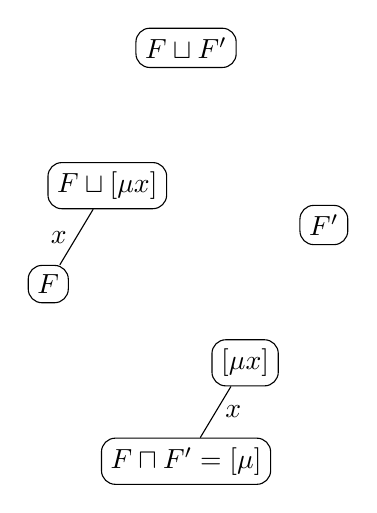
\begin{tikzpicture}
    \tikzstyle{S}=[rectangle, draw=black, rounded corners=5pt]

    \node[S] (Fp) at (1.75,.5) {$F'$};
    \node[S] (F) at (-1.75, -.25) {$F$};

    \node[S] (m) at (0, -2.5) {$F\sqcap F' =[\mu]$};
    \node[S] (mx) at (.75, -1.25) {$[\mu x]$};
    \node[S] (Fx) at (-1, 1) {$F \sqcup [\mu x]$};
    \node[S] (join) at (0, 2.75) {$F \sqcup F'$};

    \draw (m) -- (mx) node [midway, right] {$x$};
    \draw (F) -- (Fx) node [midway, left] {$x$};

    \iffalse
    \draw[dashed, gray] (mx) -- (Fp);
    \draw[dashed, gray] (m) -- (F);
    \draw[dashed, gray] (Fp) -- (join);
    \draw[dashed, gray] (Fx) -- (join);
    \fi
    \drawSolidDashedEdgeTwo{mx}{Fp};
    \drawSolidDashedEdge{m}{F};
    \drawSolidDashedEdge{Fp}{join};
    \drawSolidDashedEdgeTwo{Fx}{join};
\end{tikzpicture}
\iffalse
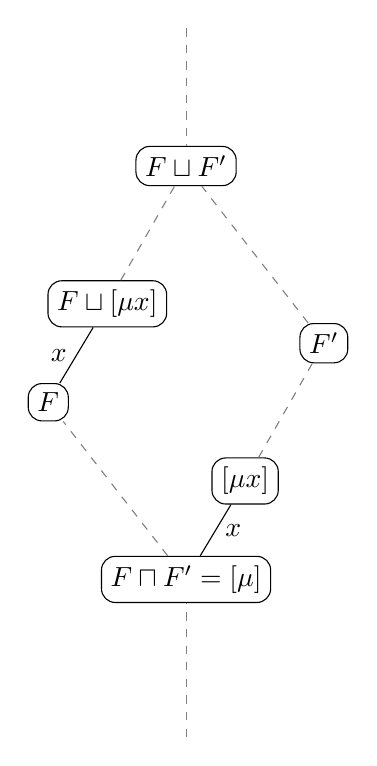
\begin{tikzpicture}
    \tikzstyle{S}=[rectangle, draw=black, rounded corners=5pt]

    \node[S] (Fp) at (1.75,.5) {$F'$};
    \node[S] (F) at (-1.75, -.25) {$F$};

    \node[S] (m) at (0, -2.5) {$F\sqcap F' =[\mu]$};
    \node[S] (mx) at (.75, -1.25) {$[\mu x]$};
    \node[S] (Fx) at (-1, 1) {$F \sqcup [\mu x]$};
    \node[S] (join) at (0, 2.75) {$F \sqcup F'$};

    \draw (m) -- (mx) node [midway, right] {$x$};
    \draw (F) -- (Fx) node [midway, left] {$x$};

    \draw[dashed, gray] (mx) -- (Fp);
    \draw[dashed, gray] (m) -- (F);
    \draw[dashed, gray] (0,-4.5) -- (m);
    \draw[dashed, gray] (0, 4.5) -- (join);
    \draw[dashed, gray] (Fp) -- (join);
    \draw[dashed, gray] (Fx) -- (join);
\end{tikzpicture}
\fi

    \caption{Above is a sublattice of $\L(\glang)$ satisfying the premise described in the Forking Lemma. We draw the covering relation by solid lines, labelled by $x$ as it is a continuation advancing words in the lower neighbor to words in the upper neighbor, and denote a flat lying below another in a way which may or may not be covering by the dotted lines. Then, $F$ and $F'$ are such that the letter $x$ is a continuation of the meet $F\sqcap F' = [\mu]$, with $[\mu x]$ lying below $F'$ but not $F$. Then, $x$ must be a continuation of $F$ as a consequence. By semimodularity $F \sqcup [\mu x]$ covers $F$, so $F \prec \kappa^{-1}(\kappa(F) + x)$ (what we just found) and $\kappa^{-1}(\kappa(F) + x) \sqsubseteq F\sqcup [\mu x]$ imply $\kappa^{-1}(\kappa(F) + x) = F\sqcup [\mu x]$.}\label{fig:forking}
\end{figure}

%In this section we show that for any aligned representation $\rho$, the flat supports are always $\rho$-closed.
%We note that many of these results will be proven under weaker premises than the existence of an aligned or integral representation.
%This is so that we can apply these results in Section~\ref{subsec:greatest} when we construct an explicit representation for every polymatroid greedoid, as we will need to start only from the assumptions of optimism and the local poset property.

Now we present our Forking Lemma for interval greedoids.
%Towards the end of the section, we use it to show that the flat supports of a polymatroid greedoid are $\rho$-closed for any aligned representation $\rho$ and that every optimistic interval greedoid is strongly optimistic.
This lemma will be frequently applied in Sections~\ref{sec:characterization} and~\ref{sec:galois} for obtaining our main results.
Furthermore, towards the end of the section we use our lemma to show that optimistic interval greedoids satisfy a stronger form of Definition~\ref{def:optimism}.

\begin{lemma}[Forking Lemma]\label{lem:forking}
    Let $\glang$ be a greedoid with the interval property, and select two flats $F, F'\in\glang/\mathord{\sim}$.
    Suppose that $\mu \in F\sqcap F'$.
    Then, $x \in \Gamma(F\sqcap F')$ and $[\mu x] \sqsubseteq F'$ implies $x \in \Gamma(F)$.
\end{lemma}

We imagine the continuation $x\in\Gamma(F\sqcap F')$ as creating a ``fork'' in that it leads to a flat beneath $F'$ but not $F$ whenever $F\neq F'$, see Figure~\ref{fig:forking}.
In some sense, the lemma thus shows that concatenation with $x$ is partially commutative.
Compare these guarantees to the exchange and interval properties:
Suppose $\alpha, \beta \in \glang$ with $|\alpha| < |\beta|$.
Then, the exchange and interval properties guarantee \emph{existence} of $x \in\widetilde{\beta}\setminus \widetilde{\alpha}$ with $x\in\Gamma[\alpha]$, but cannot guarantee a \emph{specific} identity of $x$.
In contrast, the Forking Lemma can be applied to witness a specific identity of such a continuation $x$.

To prove this result, we induct over the difference in grade between $F$ and the meet $F\sqcap F'$.
For this, we will require the following weaker result making a statement similar to the Forking Lemma, but only for words differing by one letter in the same location.
\begin{lemma}\label{lem:inner-forking}
    Let $\glang$ be a greedoid with the interval property, and $\mu \in \glang$ a feasible word.
    If there exists $x,y \in \Gamma[\mu]$ and $\alpha \in \univ^*$ with $\mu x \alpha$ and $\mu y \alpha$ feasible, then $\mu x \alpha \not\sim \mu y \alpha$ implies $\mu y \alpha x \in \glang$.
\end{lemma}
\begin{proof}
    Select $x,y \in \Gamma[\mu]$ and $\alpha \in \univ^*$ satisfying the premise.
    Note that $\mu x \alpha \not\sim \mu y \alpha$ ensures that $x \neq y$, making the task of showing $x \in \Gamma[\mu y \alpha]$ well-formed.
    To do so, first recall that two words in the same flat of an interval greedoid are cospanning.
    Hence, via negation we find $\Gamma[\mu x \alpha] \neq \Gamma[\mu y \alpha]$.
    First, suppose $\Gamma[\mu x \alpha] \setminus \Gamma[\mu y \alpha] \neq \varnothing$, and select a letter $z$ in this difference.
    Then because,
    \begin{equation}\label{eq:pidgeonhole}
        \widetilde{\mu x \alpha z} \setminus \widetilde{\mu y \alpha} = \{x, z\},
    \end{equation}
    and the words of $\glang$ are simple, the fact that $\mu x \alpha z \in \glang$ and $|\mu x \alpha z| > |\mu y \alpha|$ makes the lemma by way of the exchange axiom.
    More precisely, since $z \notin \Gamma[\mu y \alpha]$ and Eq.~\ref{eq:pidgeonhole} makes $x$ the only letter that can be concatenated onto $\mu y \alpha$ from $\widetilde{\mu x \alpha z}$ while maintaining feasibility, we conclude that $\mu y \alpha x \in \glang$.
    
    To finish, we must also verify that the case of $\Gamma[\mu x\alpha]\setminus \Gamma[\mu y \alpha] = \varnothing$ does not pose any problems.
    If this is true, then there exists $z \in \Gamma[\mu y \alpha]\setminus \Gamma[\mu x \alpha]$.
    Then, by symmetry the preceding arguments show that $\mu x \alpha y \in \glang$.
    Therefore, by simple exchange it must be the case that $\mu y \alpha x$ is feasible as well, because $|\mu x \alpha y| > |\mu y \alpha|$ and $\widetilde{\mu x \alpha y} \setminus \widetilde{\mu y \alpha} = \{x\}$.
\end{proof}
%This argument can now be extended to the generality of the Forking Lemma.
\iffalse
\begin{restatable}[Forking Lemma]{lemma}{forkinglemma}\label{lem:forking}
    Let $\glang$ be a greedoid with the interval property, and $F, F'\in\glang/\mathord{\sim}$ flats.
    Consider a feasible word $\mu \in F\sqcap F'$ in the meet.
    For all $x \in \Gamma[\mu]$, if $[\mu x] \sqsubseteq F'$ then $x \in \Gamma(F)$.
\end{restatable}
\fi
\begin{proof}[Proof of the Forking Lemma]
    Let $\mu \in \glang$ and $x \in \Gamma[\mu]$ be as described in Lemma~\ref{lem:forking}.
    Put more concisely, our assumptions make,
    $$F\sqcap F' = [\mu] \sqsubset [\mu x] \sqsubseteq F'.$$
    and from this, the reader should observe that the strict ordering relation between $[\mu]$ and $[\mu x]$ ensures $[\mu x] \not\sqsubseteq F$, thereby making $F \neq F'$ as well.
    Hence, there exists a letter $y \in \Gamma[\mu]$ and $\alpha \in \univ^*$ where $y \neq x$ and $\mu y \alpha \in F$.
    To prove the lemma, we will induct over the difference $r(F) - r[\mu]$.
    In the base case where $r(F) - r(F\sqcap F') = 1$, we see that $\alpha = \epsilon$.
    Then, because $\mu y \in F$ and $[\mu x] \not \sqsubseteq F$, it is the case that $\mu x \not\sim \mu y$.
    Therefore, by applying Lemma~\ref{lem:inner-forking} to $\mu x \epsilon$ and $\mu y \epsilon$ we find $\mu y \epsilon x = \mu y x$ is feasible, which makes the base case as this is equivalent to stating $x \in \Gamma(F)$.

    Now, recalling $\mu y \alpha \in F$, for the inductive step we make $r(F) - r[\mu] > 1$ by assuming $\alpha = \beta z$ where $z \in \univ$ is a letter and $\beta \in \univ^*$ is a simple word, possibly $\beta = \epsilon$.
    By the interval property there exists a subword of $\mu y \beta z$ of length at least $|\mu y \beta z| - |\mu x| = |\beta| + 1$ which can be concatenated onto $\mu x$ to make a feasible word.
    The resulting feasible word must be simple (no letters can be repeated), and so there are three possibilities for the identity of this observed subword:
    \begin{enumerate}
        \item The subword equals $y\beta$, and so $\mu x y \beta$ is feasible,
        \item The subword equals $\beta z$, and so $\mu x \beta z$ is feasible,
        \item There exists another subword $\beta'$ of $\beta$ resulting from the deletion of some single letter, which is to say $|\beta'| = |\beta| -1$, such that $\mu x y \beta' z$ is feasible.
    \end{enumerate}
    Suppose that either (1.) or (3.) is true.
    Then, in either of these cases the hereditary axiom makes $\mu xy$ feasible, and thus $\mu y x$ is feasible as well by exchange from $\mu xy$ to $\mu y$.
    Furthermore, $[\mu x] \not\sqsubseteq F$ implies $[\mu y x] \not\sqsubseteq F$ as well (since $[\mu x] \prec [\mu y x]$ by $y \in \Gamma[\mu x]$), and so $[\mu y] \sqsubseteq F$ makes $F \sqcap [\mu yx] = [\mu y]$ by construction.
    As a consequence,
    \[
        r(F) - r(F \sqcap [\mu y x]) = r(F) - r([\mu y]) = r(F) - r([\mu]) + 1.
    \]
    Therefore, by applying the inductive hypothesis to $F$ and $[\mu y x]$, we witness $x \in \Gamma(F)$.
    The only remaining case is (2.), where $\mu x \beta z \in \glang$.
    Here, we simply apply Lemma~\ref{lem:inner-forking} to $\mu x \beta z$ and $\mu y \beta z$ to find $\mu y \beta z x \in \glang$.
    Then, because this case makes $\mu y \beta z \in F$ we conclude that $x \in \Gamma(F)$.
\iffalse
    For the other direction, suppose that for all choices of $F,F' \in \glang/\mathord{\sim}$ we have the following: If a continuation $x \in \Gamma(F\sqcap F')$ satisfies $(F\sqcap F')\circ x \sqsubseteq F'$, then $x \in \Gamma(F)$.
    Select any feasible $\alpha, \beta \in \glang$, and assume $|\beta| > |\alpha|$.
    We will show the existence of a subword $\beta'$ of $\beta$ with length $|\beta'| \geq \delta$, for $\delta \triangleq |\beta| - |\alpha|$, such that $\alpha\beta'$ is feasible.
    To do so, first let $\beta = b_1\ldots b_k$, and let $b_1 \ldots b_i$ be the $\beta$-prefix spanning $[\alpha]\sqcap [\beta]$.
    Note, in the case where $[\alpha] \sqcap [\beta]$ is the bottom flat this prefix equals the empty word $\epsilon$, and we let $i = 0$ by convention.
    We claim that $\beta' = b_{i+1}\ldots b_{i+\delta}$ is a suitable subword for showing the interval property, i.e. that $\alpha b_{i+1}\ldots b_{i+\delta}$ is feasible.
    To show this, we will verify that
    \begin{align*}
        \alpha b_{i+1} \ldots b_{i+j}\in\glang,
    \end{align*}
    for each $j \in \{1, \ldots, \delta\}$.
    We use induction.
    The base case, where $j = 1$, follows easily:
    By construction $b_{i+1} \in \Gamma([\alpha]\sqcap[\beta])$ and,
    \[
        ([\alpha]\sqcap[\beta])\circ b_{i+1} \sqsubseteq [\beta],
    \]
    and so our initial assumptions make $\alpha b_{i+1}$ feasible.
    Now, let $j > 1$ but less than $\delta$.
    By hypothesis, we find that $\alpha b_{i+1}\ldots b_{i + j - 1}$ is feasible.
\fi
\end{proof}

By applying the Forking Lemma over an inductive structure, we can prove a stronger statement which concerns words rather than single letters.
Namely, repeated applications show the existence of words in $F\sqcup F'/F$ which are constructed from subwords of words in $F/F\sqcap F'$.

\begin{proposition}[Amplified Forking Lemma]\label{prop:amplified-forking}
    Let $\glang$ be a greedoid with the interval property, and select two flats $F, F'\in\glang/\mathord{\sim}$.
    For all $\alpha \in F/F\sqcap F'$, there exists a subword $\alpha'$ of $\alpha$ with $\alpha' \in F\sqcup F'/F$.
\end{proposition}
\begin{proof}
    Induct over $|\alpha|$.
    If $\alpha = \epsilon$, then $F\sqsubseteq F'$.
    So $F=F\sqcap F'$ and $F' = F\sqcup F'$, making $\epsilon \in F/F\sqcap F'$ and $\epsilon \in F\sqcup F'/F'$.
    Now for the inductive step, let $\alpha = \beta x$ and $F_0$ be the flat covered by $F$ which is formed by concatenating any word spanning $F\sqcap F'$ with $\beta$.
    By hypothesis, there exists a subword $\beta'$ of $\beta$ such that $\beta'\in F_0\sqcup F'/F'$.
    If $F_0\sqcup F' = F\sqcup F'$ then we are done,
    so assume $F_0\sqcup F' \neq F\sqcup F'$.
    This makes $F\not\sqsubseteq F_0\sqcup F'$, and so it follows that,
    \begin{equation}\label{eq:igiveup}
        F \sqcap (F_0\sqcup F') = F_0, 
    \end{equation}
    since $F_0 \prec F$, and $F_0$ lies below both $F$ and $F_0\sqcup F'$.
    By substitution $F \succ F \sqcap (F_0\sqcup F')$, so,
    \[
        F_0\sqcup F' \prec F \sqcup (F_0\sqcup F') = F\sqcup F',
    \]
    by semimodularity.
    Observe, because $F_0\sqcup F'$ is rank one less than $F\sqcup F'$, appending any letter in $\Gamma(F_0\sqcup F')\cap\kappa(F\sqcup F')$ to $\beta'$ leads to a word spanning $F\sqcup F'/F'$.
    Well, $\alpha = \beta x$ implies $x \in \kappa(F)$, and Eq.~\ref{eq:igiveup} shows $x$ is a continuation of the meet of $F$ and  $F_0\sqcup F'$ leading to a flat ($F$ to be precise) which is not lesser than $F_0\sqcup F'$.
    Then, by applying the Forking Lemma for $x \in \Gamma(F_0\sqcup F')$, we see that $\alpha'=\beta'x$ gives the result.
\end{proof}

\iffalse
\begin{lemma}\label{lem:k-diff-cont}
    Let $\glang$ be a normal greedoid with optimism and the interval property.
    Select flats $F,F'\in\glang/\mathord{\sim}$ such that $F\sqsubseteq F'$, and for convenience take any $\alpha \in F$.
    Then, for every letter $x \in \kappa(F')\setminus \kappa(F)$, there exists $\beta \in \glang/\alpha$ such that $x \in \Gamma[\alpha\beta]$.
    %and $[\alpha \beta x] \sqsubseteq F'$.
\end{lemma}
\begin{proof}
    Suppose $F \neq F'$ so that $\kappa(F')\setminus\kappa(F) \neq \varnothing$, and select $x \in \kappa(F')\setminus\kappa(F)$.
    Take some $\alpha \in F$, and let $\gamma \in \glang/\alpha$ be such that $\alpha\gamma \in F'$.
    Since $\kappa$ is monotone in the presence of the interval property, and $x \in \kappa[\alpha\gamma] = \kappa(F')$ by assumption, it follows that there is no suffix in $\glang/\alpha\gamma$ possessing $x$ as a letter.
    Therefore, there is a prefix of $\alpha\gamma$ possessing $x$ as a continuation.
    Suppose we name this prefix $y_1\ldots y_k$.
    %We note then that $[y_1\ldots y_k]\sqsubset F'$ since $x \in \Gamma[y_1\ldots y_k]$ by construction.
    Now, if it is the case that $k \geq |\alpha|$, meaning that $\alpha$ itself is a prefix of $y_1\ldots y_k$, then the lemma follows.
    So, suppose that $k < |\alpha|$.
    Since $x \notin \kappa[\alpha]$, by the correspondence between the flat supports and flats of an interval greedoid we have $[y_1\ldots y_k x] \not \sqsubseteq [\alpha]$.
    Hence, because $[y_1\ldots y_k]$ bounds both $[y_1\ldots y_k x]$ and $[\alpha]$ below, and $[y_1\ldots y_k x] \succ [y_1\ldots y_k]$, it follows that,
    $$[y_1 \ldots y_k] = [y_1\ldots y_k x]\sqcap [\alpha].$$
    In particular, this makes $x \in \Gamma([y_1\ldots y_k x] \sqcap [\alpha])$, so we apply our Forking Lemma for $x \in \Gamma[\alpha]$.
    Summing this up, we've shown that if there does exist some strict prefix of $\alpha$ possessing $x$ as a continuation, then taking $\beta = \epsilon$ satisfies the lemma.
    This concludes the result.
\end{proof}

Now, we can use the previous lemmas to infer an interesting relationship between the flat supports.
Specifically, call two flats $F,F'\in\glang/\mathord{\sim}$ a \emph{modular pair} whenever they witness the submodular law on $\L(\glang)$ with equality, i.e.,
\[
    r(F) + r(F') = r(F\sqcap F') + r(F\sqcup F').
\]
By applying optimism in combination with the Forking Lemma, we will find that the flat support of the meet of a modular pair is equal to the intersection of the flat supports.
%This insight will play a key role in our embedding of the flats into a geometric lattice, presented in Section~\ref{subsec:embedding}.

\begin{proposition}\label{prop:mod-k-closed}
    Let $\glang$ be a normal greedoid with optimism and the interval property.
    Select flats $F, F'\in\glang/\mathord{\sim}$.
    If $F$ and $F'$ are a modular pair, then the flat support of their meet is equal to the intersection of their flat supports.
    More precisely,
    \[
        r(F)+r(F') = r(F\sqcap F') + r(F\sqcup F') \implies \kappa(F\sqcap F') = \kappa(F) \cap \kappa(F').
    \]
\end{proposition}
\begin{proof}
    Let $F$ and $F'$ be a modular pair.
    We note that $\kappa(F\sqcap F') \subseteq \kappa(F) \cap \kappa(F')$ is a result of the flat support closure over the flats $\kappa:\L(\glang)\to\left(2^\univ,\subseteq\right)$ being order-preserving.
    So, to show the reverse inclusion select $x \in \kappa(F) \cap \kappa(F')$.
    By way of contradiction, let $x \notin \kappa(F\sqcap F')$.
    Then, letting $\mu \in F\sqcap F'$, since $x \in \kappa(F) \setminus \kappa(F\sqcap F')$ we can apply Lemma~\ref{lem:k-diff-cont} to ensure the existence of some $\beta \in \glang/\mu$ such that $x \in \Gamma[\mu \beta]$ and $[\mu\beta x]\sqsubseteq F$.
    In light of the latter conjunct, also fix $\gamma \in \glang/\mu\beta x$ such that $\mu\beta x \gamma \in F$.
    Now, without loss of generality suppose that $r(F) \leq r(F')$, and let $\beta x \gamma = y_1\ldots y_k$.
    Selecting $\alpha \in \glang/\mu$ so that $\mu \alpha \in F'$, we induct over $i \leq k$ to show that $\mu\alpha y_1\ldots y_i$ is always feasible word.
    Suppose $i = 1$, then the result follows by the Forking Lemma.
    Now, for the inductive step, observe that $\mu\alpha\beta y_1\ldots y_{i-1}$ is feasible by hypothesis.
    The monotonicity of $\kappa:2^\univ\to 2^\univ$ in the presence of the interval property implies,
    \[
        \kappa[\mu y_1 \ldots y_{i-1}] = \kappa(\widetilde{\mu} \cup \{y_1,\ldots, y_{i-1}\}) \subseteq \kappa(\widetilde{\mu} \cup \widetilde{\alpha} \cup \{y_1,\ldots, y_{i-1}\}) = \kappa[\mu \alpha y_1\ldots y_{i-1}].
    \]
    Thus, $[\mu y_1\ldots y_{i-1}] \sqsubseteq [\mu \alpha y_1\ldots y_{i-1}]$ meaning that,
    \begin{equation}\label{eq:3333}
        [\mu y_1\ldots y_{i-1}] \sqsubseteq F\sqcap [\mu \alpha y_1\ldots y_{i-1}] 
    \end{equation}
    Furthermore, observe,
    \begin{align*}
        r[\mu y_1\ldots y_{i- 1}] = r(F\sqcap F') + i - 1,&&\text{and},&& r[\mu\alpha y_1\ldots y_{i-1}] = r(F') + i - 1,
    \end{align*}
    and so by combining the above with the fact that $F$ and $F'$ are a modular pair,
    \begin{equation}\label{eq:2222}
        r(F) + r[\mu\alpha y_1\ldots y_{i-1}] = r[\mu y_1 \ldots y_{i-1}] + r(F\sqcup F').
    \end{equation}
    Then, take note that $\kappa[\mu\alpha y_1\ldots y_{i-1}] \subseteq \kappa(F) \cup \kappa(F') \subseteq \kappa(F\sqcup F')$, and so $[\mu\alpha y_1\ldots y_{i-1}]\sqsubseteq F\sqcup F'$.
    It follows then that $F \sqcup [\mu\alpha y_1\ldots y_{i-1}] = F\sqcup F'$, as if there was a lesser upper bound of these flats then $[\mu \alpha y_1\ldots y_{i-1}] \sqsupseteq F'$ would imply an upper bound of $F$ and $F'$ which is lesser than $F\sqcup F'$.
    In light of this observed identity of the join, when we combine Eq.s~\ref{eq:3333} and~\ref{eq:2222} we witness,
    \begin{equation}\label{eq:7777}
        F\sqcap [\mu\alpha y_1\ldots y_{i-1}] = [\mu\alpha y_1\ldots y_{i-1}],
    \end{equation}
    as if there existed a common lower bound of $F$ and $[\mu\alpha y_1\ldots y_{i-1}]$ greater than $[\mu y_1\ldots y_{i-1}]$, then the submodular law on $\L(\glang)$ would be violated.
    Finally, note that $[\mu y_1 \ldots y_i] \not\sqsubseteq [\mu\alpha y_1\ldots y_{i-1}]$ because $[\mu y_1\ldots y_i] \sqsubseteq F$ and Eq.~\ref{eq:7777} shows $[\mu y_1\ldots y_i] \sqsupset F \sqcap [\mu\alpha y_1\ldots y_{i-1}]$.
    In fact, we have the covering relation $[\mu y_1 \ldots y_i] \succ [\mu y_1\ldots y_{i-1}]$,
    and so since $[\mu y_1\ldots y_{i-1}]$ bounds both of the incomparable flats $[\mu y_1\ldots y_i]$ and $[\mu \alpha y_1 \ldots y_{i-1}]$ below it follows that,
    \[
        [\mu y_1\ldots y_{i-1}] = [\mu y_1 \ldots y_i]\sqcap [\mu \alpha y_1 \ldots y_{i-1}].
    \]
    Hence, since $y_i \in \Gamma[\mu y_1\ldots y_{i-1}]$ we apply our Forking Lemma to find that $y_i \in \Gamma[\mu\alpha y_1\ldots y_{i-1}]$.
    Therefore, by the principle of induction we find that $y_1\ldots y_k \in \glang/\mu\alpha$.
    Now, since there exists a $j \in \{1,\ldots,k\}$ such that $x = y_j$, it follows by the monotonicity of $\kappa:2^\univ\to 2^\univ$ in the presence of the interval property that $x \notin \kappa[\mu\alpha]$.
    However, recall that we constructed the word $\mu\alpha$ so that $\mu\alpha \in F'$, so we have found $x \notin\kappa(F')$.
    This contradicts our assumption that $x \in \kappa(F)\cap\kappa(F')$, and so the proposition follows.
\end{proof}

    Matroids provide a clear example that the converse does not hold.
    This is because the flat supports of a normal matroid are equal to its closed sets.
    Then, being a closure system, the flat supports of a normal matroid are thus always closed under intersection.
    Now, within the class of semimodular lattices, it is known that our rank based definition of modular pairs is equivalent to the lattice theoretic definition, being those pairs satisfying the diamond isomorphism theorem.
    A modular lattice is one such that every pair of elements satisfies this criteria.
    Hence, if the converse were true then the lattice of flats of any normal matroid would be modular, which is generally not true.
    %For insight on the last point, within the class of semimodular lattices it is generally known that satisfying the submodular law with equality is equivalent to a pair satisfying the diamond isomorphism theorem \cite{stanley}.
    %The class of modular lattices 
\textcolor{red}{Use this to simplify the proof of the above proposition}
\fi
\iffalse
Now, we can use the previous lemmas to infer a significant relationship between the flat supports.
Specifically, call two flats $F,F'\in\glang/\mathord{\sim}$ a \emph{modular pair} whenever they witness the submodular law on $\L(\glang)$ with equality, i.e.,
\[
    r(F) + r(F') = r(F\sqcap F') + r(F\sqcup F').
\]
In Proposition~\ref{prop:mod-k-closed}, we will show the flat support of the meet of a modular pair is equal to the intersection of the flat supports of the flats forming the pair.
But, first we show a useful technical lemma stating that given a modular pair, the suffixes going from the meet to these flats can always be composed together.
This statement will be made more precise in what comes.
Finally, we point out that by way of the Forking Lemma, this interesting behavior holds by only assuming the interval property.
\begin{lemma}\label{lem:modular-concatenation}
    Let $\glang$ be a normal greedoid with the interval property.
    Select flats $F, F'\in\glang/\mathord{\sim}$ such that $F$ and $F'$ make a modular pair, and let $\mu\in F\sqcap F'$ be any word in their meet.
    Then, for all $\alpha,\beta \in \univ^*$ such that $\mu \alpha \in F$ and $\mu\beta \in F'$, we have that $\mu \alpha \beta$ is feasible.
\end{lemma}
\begin{proof}
    Induct over $r(F') - r(F\sqcap F')$.
    When this difference is zero, we find $F' = F\sqcap F'$.
    Then, the base case is trivial since this makes $\beta = \epsilon$.
    Now, assume $F' \sqsupset F\sqcap F'$ and let $\beta = \beta' x$.
    To allow ourselves to apply our inductive hypothesis, we verify that $F$ and $[\mu\beta']$ make a modular pair.
    Well, note that $F\sqcap [\mu\beta']\sqsubseteq F\sqcap F'$, and so since $F\sqcap F'$ lies below both of $F$ and $[\mu\beta']$ it follows that $F\sqcap[\mu\beta'] = F\sqcap F'$.
    Furthermore,
    \begin{equation}\label{eq:hfgw}
        r(F) + r[\mu\beta'] \geq r(F\sqcap [\mu\beta']) + r(F\sqcup [\mu\beta']) = r(F\sqcap F') + r(F\sqcup [\mu\beta']).
    \end{equation}
    And so, $[\mu\beta'] \prec [\mu\beta] = F'$ implies $r(F) + r[\mu\beta'] = r(F) + r(F') - 1$.
    Therefore, because $F$ and $F'$ make a modular pair by assumption, combining our previous observation with Eq.~\ref{eq:hfgw} makes,
    \[
        r(F\sqcap F') + r(F\sqcup F') - 1 \geq r(F\sqcap F') + r(F\sqcup [\mu\beta']).
    \]
    This means that $F\sqcup [\mu\beta'] \sqsubset F\sqcup F'$, which implies $F'\not\sqsubseteq F\sqcup [\mu\beta']$.
    In light of this we have $F'\sqcap \left(F\sqcup [\mu\beta']\right) \sqsubseteq F'$, and so as $F'\succ [\mu\beta']$ and $[\mu\beta']\sqsubseteq F\sqcup [\mu\beta']$ it follows that,
    \[
        F'\sqcap \left(F\sqcup [\mu\beta']\right) = [\mu\beta'].
    \]
    However, this means that $F'$ covers its meet with $F\sqcup [\mu\beta']$, and so by the semimodularity of the flats of an interval greedoid it follows that $F'\sqcup\left(F\sqcup [\mu\beta']\right)$ covers $F\sqcup [\mu\beta']$.
    Well, lattice operations are communative and associative (see any of \cite{davey2002introduction, garg2015introduction,gratzer2011lattice} for more information), and so,
    \[
        F'\sqcup\left(F\sqcup [\mu\beta']\right) = F\sqcup\left(F' \sqcup [\mu\beta']\right) = F\sqcup F'.
    \]
    Therefore, our observations make $F\sqcup [\mu\beta'] \prec F\sqcup F'$, and by applying our assumption that $F$ and $F'$ make a modular pair we witness,
    \[
        r(F) + r[\mu\beta'] = r(F) + r(F') - 1 = r(F\sqcap F') + r(F\sqcup F') - 1 = r(F\sqcap [\mu\beta']) + r(F\sqcup [\mu\beta']).
    \]
    This makes $F$ and $[\mu\beta']$ a modular pair.

    Now with that done, we see that $\mu \alpha \beta'$ is feasible by inductive hypothesis.
    Since greedoids are simple languages, this means that $\widetilde{\alpha}\cap\widetilde{\beta'} = \varnothing$.
    Therefore, 
    \[
        |\widetilde{\mu\alpha\beta'}| = |\widetilde{\mu}| + |\widetilde{\alpha}| + |\widetilde{\beta'}| = |\widetilde{\mu\alpha}| + |\widetilde{\mu\beta}| - 1 - |\widetilde{\mu}| = r(F) + r(F') - 1 - r(F\sqcap F') = r(F\sqcup F') - 1.
    \]
    And so, $[\mu\alpha\beta'] \prec F\sqcup F'$.
    As a consequence, $F'$ cannot be lesser than $[\mu\alpha\beta']$ as if this were true then the join $F\sqcup F'$ could be no greater than $[\mu\alpha\beta']$ since $F = [\mu\alpha]\sqsubseteq [\mu\alpha\beta']$.
    Then, because $[\mu\beta'] \prec F'$ and $[\mu\beta'] \sqsubseteq [\mu\alpha\beta']$ by exchange, it can only be that $F' \sqcap [\mu\alpha\beta'] = [\mu\beta']$.
    We see then that $x \in \Gamma[\mu\beta']$ is a continuaton such that $[\mu\beta' x] = F \not\sqsubseteq [\mu\alpha\beta']$, and so by the Forking Lemma $\mu\alpha\beta' x$ is feasible.
    One then concludes the lemma by substituting $\beta = \beta' x$.
\end{proof}

Now, by adding optimism as an assumption we can use the prior lemma to prove that the meet of a modular pair has a flat support equal to the intersection of the flat supports of the flats giving the pair.

\fi

The Forking Lemma combines nicely with optimism to show that flat supports witness the feasibility of eventually appending a letter $y$ onto some extension of a feasible word $\alpha$.
In particular, $y\notin\kappa[\alpha]$ implies the existence of $\beta \in \glang/\alpha$ with $\alpha\beta y$ feasible.
In many ways, this is a generalization of the matroid fact that points beyond the span of an independent set can be used to obtain a larger independent set, and
so is a pleasant example of polymatroid greedoids lying between matroids and general greedoids in terms of their axiomatic power.

\begin{proposition}\label{prop:strong-opt}
    Let $\glang$ be a greedoid with the interval property.
    If $\glang$ is optimistic, then for all $\alpha \in \glang$, $y \notin \kappa[\alpha]$ implies the existence of $\beta \in \glang/\alpha$ with $y\in \widetilde{\beta}$.
\end{proposition}
\begin{proof}
    By optimism, at least one of the following are true:
    There exists an $\alpha$-prefix $\alpha'$ such that $y \in \Gamma[\alpha']$, or there exists $\beta\in\glang/\alpha$ with $y \in \widetilde{\beta}$.
    The latter is our target statement, so suppose the former is true.
    Because $y \notin \kappa[\alpha]$ implies $[\alpha'y] \neq [\alpha]$, it is the case that $[\alpha'y]\sqcap [\alpha] \sqsubset [\alpha'y]$.
    Observe, $[\alpha']$ lies below both $[\alpha'y]$ and $[\alpha]$.
    So, since $[\alpha'y]$ covers $[\alpha']$, it follows that $[\alpha'] = [\alpha' y] \sqcap [\alpha]$.
    Hence, we may apply the Forking lemma to $[\alpha'y]$ and $[\alpha]$ to see $y \in \Gamma[\alpha]$.
    Thus $y\in\glang/\alpha$, so the word $\beta = y$ satisfies the proposition.
\end{proof}


\iffalse
Finally, we use the Forking Lemma in conjunction with results of the previous section to prove a deep connection between the flats of a polymatroid greedoid and the closed sets of its aligned representations.
For this, with Lemmas~\ref{lem:aaligned-mr} and~\ref{lem:step->continuation}, we first show that any feasible $\alpha \in \glang$ makes the marginal return of letters beyond its flat support $\kappa[\alpha]$ no less than one.
%This is a useful insight for arguments making use of the marginal returns of aligned representations, and when combined with Lemma~\ref{lem:aaligned-mr} shows that flat supports of a polymatroid greedoid determine the closure operator of the representation.
Then as a consequence, the flat supports of the polymatroid greedoid make closed sets in any of its aligned representations.

\begin{theorem}\label{thm:flat supports-are-closed}
    Let $\glang$ be a normal greedoid, and suppose that $\glang$ possesses an aligned representation $\rho$.
    Select any flat $F\in\glang/\mathord{\sim}$.
    Then, the flat support $\kappa(F)$ is $\rho$-closed, i.e. $\sigma_\rho(\kappa(F)) = \kappa(F)$.
\end{theorem}
\begin{proof}
    First, let $\alpha\in\glang$.
    We show, for all $x \in \univ$,
    \begin{equation}\label{eq:4ghti}
        x\notin\kappa[\alpha] \iff (\rho/\widetilde{\alpha})(x) \geq 1.
    \end{equation}
    Lemma~\ref{lem:aaligned-mr} ensures $x \in \kappa[\alpha]$ implies $(\rho/\widetilde{\alpha})(x) = 0$.
    So, for the other direction let $\alpha \in \glang$ and $y \in \univ$ be such that $y \notin \kappa[\alpha]$.
    By way of contradiction suppose $(\rho/\widetilde{\alpha})(y) < 1$.
    Then, by Lemma~\ref{lem:aaligned-mr} makes $(\rho/\widetilde{\alpha})(y) = 0$.
    Because $\glang$ is normal there exists a feasible word containing $y$, meaning that one witnesses $\rho(y) = (\rho/\widetilde{\epsilon})(y) \geq 1$ by the law of diminishing returns.
    Hence, letting $\alpha = x_1\ldots x_{|\alpha|}$, there must be some index $i \in \{1,\ldots, |\alpha|\}$ such that the corresponding prefix satisfies,
    \begin{align*}
        (\rho/\{x_1,\ldots,x_i\})(y) \neq 0,&&\text{and,}&&(\rho/\{x_1,\ldots,x_{i+1}\})(y) = 0.
    \end{align*}
    Hence, by Lemma~\ref{lem:step->continuation} we observe that $x_1\ldots x_i y$ is feasible.
    But, by Proposition~\ref{prop:representation->local-poset} it follows that $\glang$ possesses the interval property.
    Furthermore,
    \[
        [x_1\ldots x_i y] \succ [x_1\ldots x_i] = [\alpha] \sqcap [x_1 \ldots x_i y],
    \]
    and $[x_1\ldots x_i y] \not \sqsubseteq [\alpha]$, both due to our assumption that $y \notin \kappa[\alpha]$.
    But, by the Forking Lemma we find that $y$ is a continuation of $\alpha$.
    So $(\rho/\widetilde{\alpha})(y) = 1$ and $(\rho/\widetilde{\alpha})(y) < 1$, a contradiction.
    Hence Eq.~\ref{eq:4ghti}.

    Now we use Eq.~\ref{eq:4ghti} to show $\kappa[\alpha]$ is $\rho$-closed.
    Note that $\widetilde{\alpha}\subseteq\kappa[\alpha]$ and $\rho(\widetilde{\alpha}) = \rho(\kappa[\alpha])$ by the interval property and Lemma~\ref{lem:aaligned-mr}, respectively.
    This implies $\sigma_\rho(\widetilde{\alpha}) = \sigma_\rho(\kappa[\alpha])$.
    Therefore, Eq.~\ref{eq:4ghti} makes $(\rho/\kappa[\alpha])(x)$ nonzero for all $x\notin\kappa[\alpha]$, so it follows that $\kappa[\alpha]$ is $\rho$-closed.
\end{proof}

It is noting that the previous result shows that the flat support structure of a polymatroid greedoid generalizes that of a normal matroid, since the flat supports of a normal matroid are equal to its closed sets (see Section~\ref{sec:preliminaries}) and the natural polymatroid representation of a matroid is its own rank function.


Finally, with our Forking Lemma we show every optimistic interval greedoid is strongly optimistic.
By Proposition~\ref{prop:int->aligned}, this of course applies to polymatroid greedoids.

\begin{proposition}\label{prop:int->strong-opt}
    Let $\glang$ be a greedoid, and suppose $\glang$ possesses the interval property.
    If $\glang$ is optimistic, then $\glang$ is strongly optimistic.
\end{proposition}
\begin{proof}
    Fix a basic word $x_1\ldots x_r\in\glang$ and a letter $y$.
    Because $\glang$ is optimistic, there is some index $i\in\{1,\ldots, r-1\}$ such that $y\in\Gamma[x_1\ldots x_i]$.
    Fix $i$ to be the smallest such index, and let $j \in \{i,\ldots, r-1\}$ satisfy $y \notin\kappa[x_1\ldots x_j]$.
    Then $y \in\kappa[x_1\ldots x_i y]$ implies $[x_1\ldots x_i y] \not\sqsubseteq[x_1\ldots x_j]$.
    Therefore, because $[x_1\ldots x_i]$ lies below both of these flats and $[x_1\ldots x_i] \prec [x_1\ldots x_i y]$, it follows that $[x_1\ldots x_j] \sqcap [x_1\ldots x_j y] = [x_1\ldots x_j]$.
    Hence by the Forking Lemma, we find $y\in\Gamma[x_1\ldots x_j]$.
\end{proof}
\fi

\section{Polymatroid Greedoids and the Greedy Algorithm}\label{sec:characterization}
\begin{algorithm*}[t]
    \DontPrintSemicolon
    \small
    $\alpha\gets\epsilon$\;
    \While{$\Gamma[\alpha]\neq\varnothing$}
    {
        $x \gets \argmin_{y\in\Gamma[\alpha]}w(y)$\;
        $\alpha\gets\alpha x$\;
    }
    \;
    \Return $\alpha$
    \caption{The Greedy Algorithm}\label{alg:greedy}
\end{algorithm*}

Let $w: \univ\to\mathbb{R}$ be a function assigning weights to the alphabet.
Suppose we wish to solve a linear optimization over the basic words of the greedoid as defined by this weight function:
\begin{equation}\label{prog:lin-greedoid}
    \def\arraystretch{1.25}
    \begin{array}{lll}
        \text{minimize}  & \sum_{x \in\widetilde{\alpha}}w(x),\quad & \\
        \text{subject to}& \alpha\in\glang, \quad & \\
                         & r[\alpha] = r(\glang). \quad &
    \end{array}
\end{equation}
This is of course an abstraction of matroid optimization, where the greedoid can be used to encode more complex constraints.
Consider the greedy algorithm:
Maintain a solution $\alpha$, initially $\alpha=\epsilon$, and grow over $r(\glang)$ rounds.
In each round, if $\Gamma[\alpha]=\varnothing$ then terminate.
Else, select a continuation $x$ of minimum weight and repeat on $\alpha x$.
%The correctness of this approach is equivalent to being sufficiently ``matroid-like.''
Korte and Lovász showed that the correctness of this approach is logically equivalent to the greedoid being sufficiently ``matroid-like.''

\begin{theorem}[\cite{korte1984greedoids}]\label{thm:greedy}
    Let $\glang$ be a greedoid with rank and basis ranks functions $r,b:2^\univ\to\mathbb{Z}$.
    The greedy algorithm correctly outputs the basic word minimizing $\alpha\mapsto \sum_{x\in\widetilde{\alpha}}w(x)$ for every weighting $w:\univ\to\mathbb{R}$ if and only if $b$ is a matroid rank function such that every $r$-closed set is $b$-closed.
\end{theorem}

In \cite{korte1984greedoids,goetschel1986linear} this is shown to be equivalent to greedoids possessing the \emph{strong-exchange property}, which we use in Appendix~\ref{app:greedy-minors}.
For this reason, we refer to greedoids for which the greedy algorithm is guaranteed to correctly solve Program~\ref{prog:lin-greedoid} \emph{strong exchange greedoids}.
Theorem~\ref{thm:greedy} shows such greedoids have a structure associated with a polymatroid rank function, i.e. its basis rank.
We use this to construct an aligned representation of any local poset greedoid with the strong-exchange property.
This will give the following:

\begin{theorem}\label{thm:lp-greedy=>pm-greedoid}
    Let $\glang$ be a greedoid with the local poset property,
    and suppose the greedy algorithm correctly solves any linear optimization over the basic words.
    Then, there exists an aligned polymatroid representation $\rho:2^\univ\to\mathbb{R}$ of $\glang$.
\end{theorem}

Our proposed representation $\greedyrep$ follows: First, define $b_F:2^\univ\to\mathbb{Z}$ to be the basis rank of the minor $\glang/F$, i.e. $b_F(X)\triangleq \max_{\alpha\in\glang/F}|\widetilde{\alpha}\cap X|.$
Then, $\greedyrep$ is defined as the constrained optimization,
\begin{align*}
    \greedyrep(X) \triangleq \min_{F\in\glang/\mathord{\sim}}\left\{\psi_F(X)\mid (\exists \alpha \in F)\;\widetilde{\alpha}\subseteq X\right\},&&\text{and},&&\psi_F(X) \triangleq r(F) + \left(1+\frac{1}{r(\glang)+1}\right)\cdot b_F(X).
\end{align*}
Observe that the minimization is constrained to flats containing a word supported by letters in $X$.
This assertion and its resulting structure will be required in our technical lemmas.
In this spirit, refer to any flat containing a word supported by $X$ as \emph{$\greedyrep(X)$-feasible}, and call a $\greedyrep(X)$-feasible flat minimizing $F\mapsto \psi_F(X)$ among other feasible flats \emph{$\greedyrep(X)$-optimal}.
Now, see that the cost function $F\mapsto\psi_F(X)$ is the flat's rank ``penalized'' by one's ability to use $X$ to construct $(\glang/F)$-feasible words.
This penalty is encoded by the minor's basis rank, so is minimal (i.e. zero) when $X\subseteq\kappa(F)$ and maximal (i.e $r(\glang)-r(F)$) when $X$ contains the support of a $(\glang/F)$-basic word.
We weigh $b_F(X)$ by a factor $1+\frac{1}{r(\glang)+1}$ greater than one to introduce marginal returns which are not equal to one whenever evaluated against the support of a feasible word $\alpha\in\glang$ on a letter $x\notin\Gamma[\alpha]$.
%Then, $\greedyrep$ is not integral.
Furthermore,
\begin{equation}\label{eq:floor-psi}
    \lfloor \psi_F(X) \rfloor = r(F) + b_F(X),\quad\forall (X,F) \in 2^\univ\times\glang/\mathord{\sim},
\end{equation}
as it is always true that $b_F(X) \leq r(\glang)$.

\begin{remark}
    Take note that the basis rank by itself is not strong enough to constitute a representation (whenever it is submodular) since $\alpha\in\glang$ and $(b/\widetilde{\alpha})(x)=1$ does not imply $x \in\Gamma[\alpha]$.
\end{remark}

\begin{figure}
\begin{floatrow}
\capbtabbox[0.5\textwidth]{%
    \centering
    \renewcommand{\arraystretch}{1.25}
    \scalebox{.8}{\begin{tabular}{|c c || c  c|} 
     \hline
     $X$ & $\rho(X)$ & $X$ & $\rho(X)$ \\
     \hline\hline
     $\varnothing$ & 0 & $\{b, c\}$ & $2 + \frac{2}{r(\glang) + 1}$\\[2pt]
     \hline
     $\{a\}$ & 1 & $\{b, d\}$ & $2 + \frac{2}{r(\glang) + 1}$ \\[2pt]
     \hline
     $\{b\}$ & $1 + \frac{1}{r(\glang) + 1}$ & $\{c, d\}$ & $2 + \frac{2}{r(\glang) + 1}$\\[2pt]
     \hline
     $\{c\}$ & $1 + \frac{1}{r(\glang) + 1}$ & $\{a,b,c\}$ & 3 \\[2pt]
     \hline
     $\{d\}$ & $1 + \frac{1}{r(\glang) + 1}$ & $\{a,b,d\}$ & 3 \\[2pt] 
     \hline
     $\{a,b\}$ & $2 + \frac{1}{r(\glang) + 1}$ & $\{a,c,d\}$ & 3 \\[2pt]
     \hline
     $\{a,c\}$ & 2 & $\{b,c,d\}$ & $2 + \frac{2}{r(\glang) + 1}$ \\[2pt]
     \hline
     $\{a,d\}$ & 2 & $\{a,b,c,d\}$ & 3 \\[2pt]
     \hline
\end{tabular}}
}{%
    \caption{Values of $\greedyrep$ when applied to the greedoid in Figure~\ref{fig:ubg}.}\label{table:greedy-rep}%
}\ffigbox[0.5\textwidth]{%
    \centering
    \scalebox{.8}{\input{tikz/gr-spans.tikz}}
}{%
    \caption{The Hasse diagram of the closed sets\\of $\greedyrep$ from Table~\ref{table:greedy-rep}, ordered by containment.}\label{fig:greedy-rep}%
}
\end{floatrow}
    %\caption{A graph with root $s$ and the lattice of flats of the corresponding undirected branching greedoid. We see that $[ac]\sqcap[ad] = [a]$ because $ac \not\sim ad$, for example. Furthermore, the reader should note (or convince themselves) that the top flat of a greedoid is always given by the basic words. 
    %Finally, if edges are weighted lexicographically the greedy basis is $adc$.
    %}\label{fig:ubg-rep}
\end{figure}

As a concrete example, we show the values taken by $\greedyrep$ over the undirected branching greedoid from Figure~\ref{fig:ubg} and its lattice of closed sets in Figure~\ref{fig:greedy-rep}.
The reader should compare with Figure~\ref{fig:ubg-rep}.
Observe that $\greedyrep(\widetilde{\alpha}) = \psi_{[\alpha]}(\widetilde{\alpha})$ for every feasible word $\alpha$ in this example, so $x\in\Gamma[\alpha]$ implies $(\greedyrep/\widetilde{\alpha})(x) = 1$ while $x \notin\Gamma[\alpha]$ implies $(\greedyrep/\widetilde{\alpha})(x)$ equals 0 or $1+\frac{1}{r(\glang)+1}$.
This relationship is true in general.

\begin{proposition}\label{prop:greedy-aligned-rep}
    Let $\glang$ be a greedoid with the interval property.
    Suppose the greedy algorithm correctly solves any linear optimization on $\glang$.
    Then, for all feasible words $\alpha \in \glang$ and $x\in\univ$,
    \[
        x \in \Gamma[\alpha] \iff \left(\greedyrep/\widetilde{\alpha}\right)(x) = 1,
    \]
    and $\left(\greedyrep/\widetilde{\alpha}\right)(x) \in \{0\}\cup[1,\infty)$. 
\end{proposition}
\begin{proof}
    First, we show $\greedyrep(\widetilde{\alpha}) = \psi_{[\alpha]}(\widetilde{\alpha})$ for all $\alpha \in \glang$.
    Select any $\greedyrep(\widetilde{\alpha})$-optimal flat, i.e. some $F\in\glang/\mathord{\sim}$ achieving $\greedyrep(\widetilde{\alpha}) = \psi_F(\widetilde{\alpha})$ such that there exists $\beta \in F$ with $\widetilde{\beta}\subseteq\widetilde{\alpha}$.
    Through the exchange axiom there is some $\gamma \in (\widetilde{\alpha}\setminus\widetilde{\beta})!$ such that $\gamma\in\glang/F$.
    Hence,
    $$b_F(\widetilde{\alpha})\geq|\widetilde{\gamma}\cap\widetilde{\alpha}| = |\gamma| = |\alpha| - r(F).$$
    Applying this to the definition of $\psi_F$ and rearranging terms shows,
    $$\psi_{F}(\widetilde{\alpha}) \geq r(F) + \left(1+\frac{1}{r(\glang) + 1}\right)\cdot\left(|\alpha| - r(F)\right) = |\alpha| + \frac{1}{r(\glang) + 1}\cdot\left(|\alpha| - r(F)\right)\geq |\alpha|.$$
    But $\psi_{[\alpha]}(\widetilde{\alpha}) = |\alpha|$, so our assumptions require $\psi_F(\widetilde{\alpha}) \leq |\alpha|$ also hold.
    Thus, $\greedyrep(\widetilde{\alpha}) = \psi_{F}(\widetilde{\alpha}) = |\alpha|$.

    Now fix $x \in \univ$.
    Notice, if $x \in\Gamma[\alpha]$ then $\alpha x$ is feasible.
    So, our preceding argument shows the desired $x \in\Gamma[\alpha]$ implies $\greedyrep(\widetilde{\alpha x}) - \greedyrep(\widetilde{\alpha}) = 1$.
    Then, for the other direction assume $x \notin\Gamma[\alpha]$.
    Once again select a $\greedyrep(\widetilde{\alpha})$-optimal flat $F$, and let $\beta\in F$ be any word with $\widetilde{\beta}\subseteq\widetilde{\alpha}$.
    Observe $x\notin\widetilde{\beta}$, as otherwise the word $\beta'x$ is a $\beta$-prefix for some subword $\beta'$ of $\beta$.
    Then, applying the Forking Lemma to $[\beta' x]$ and $[\alpha]$ (take note that $[\beta']\sqsubseteq [\alpha]$ and $[\beta'x]\succ[\beta']$ implies $[\beta']=[\alpha]\sqcap[\beta'x]$) shows $x\in \Gamma[\alpha]$, a contradiction.
    Hence $\widetilde{\beta}\subseteq\widetilde{\alpha}$, which implies $[\beta]\sqsubseteq [\alpha]$.
    Then, recalling that our assumptions about the greedy algorithm ensure that $b$ satisfies the law of diminishing returns, by way of Lemma~\ref{prop:bf} one finds $\left(b_{F}/\widetilde{\alpha}\right)(x)=\left(b_{[\beta]}/\widetilde{\alpha}\right)(x) \geq \left(b_{[\alpha]}/\widetilde{\alpha}\right)(x)$.
    So by combining this with $[\alpha]$ being $\greedyrep(\widetilde{\alpha})$-optimal,
    \begin{multline*}
        \psi_{F}(\widetilde{\alpha}+ x) = r(F) + \left(1 + \frac{1}{r(\glang) + 1}\right)\cdot b_F(\widetilde{\alpha}) +\left(1 + \frac{1}{r(\glang) + 1}\right)\cdot \left(b_{F}/\widetilde{\alpha}\right)(x),\\\geq \psi_{[\alpha]}(\widetilde{\alpha}) + \left(1 + \frac{1}{r(\glang) + 1}\right)\cdot \left(b_{F}/\widetilde{\alpha}\right)(x) = \psi_{[\alpha]}(\widetilde{\alpha}+x).
    \end{multline*}
    Thus $[\alpha]$ is $\greedyrep(\widetilde{\alpha}+x)$-optimal as well.
    So, as $\left(\greedyrep/\widetilde{\alpha}\right)(x) = \psi_{[\alpha]}(\widetilde{\alpha}+x) - \psi_{[\alpha]}(\widetilde{\alpha})$, we see $x\notin\Gamma[\alpha]$ implies $\left(\greedyrep/\widetilde{\alpha}\right)(x) \neq 1$ by,
    \begin{equation*}
        \psi_{[\alpha]}(\widetilde{\alpha}+x) - \psi_{[\alpha]}(\widetilde{\alpha}) = \begin{cases}
            1 + \frac{1}{r(\glang) + 1},\quad&\text{if }b_{[\alpha]}(x) \neq 0,\\
            0,&\text{otherwise}.
        \end{cases}
    \end{equation*}
    And we've already seen $\left(\greedyrep/\widetilde{\alpha}\right)(x) = 1$ whenever $x \in\Gamma[\alpha]$, so $\left(\greedyrep/\widetilde{\alpha}\right)(x) \in \{0\}\cup[1,\infty)$ holds too.
\end{proof}

The previous proposition will be used to show $\greedyrep$ is an aligned representation whenever $\greedyrep$ is a polymatroid rank function.
Since $\greedyrep$ is clearly normalized, we need only show monotonicity and submodularity.
To do so, we begin in Section~\ref{subsec:bf-rank} by proving facts about the function $b_F$.
Here, our main insight is that the basis rank $b_F$ of the minor $\glang/F$ can be equated with the (polymatroidal) contractions $b/\kappa(F)$.
With this, we will leverage the law of diminishing returns when analyzing $\greedyrep$.
This analysis occurs in Section~\ref{subsec:greedy-aligned-rep}, where we complete the proof of Theorem~\ref{thm:lp-greedy=>pm-greedoid} by verifying $\greedyrep$ is monotone and submodular.

\subsection{The Basis Rank of the Contraction Minors of Interval Greedoids}\label{subsec:bf-rank}
Our main result of this section is the following, equating the values of $b_F$ to those of $b/\kappa(F)$.
\begin{proposition}\label{prop:bf}
    Let $\glang$ be a greedoid with the interval property.
    Then, $b_F = b/\kappa(F)$ everywhere.
\end{proposition}
\begin{proof}
    Select an arbitrary set of letters $X\subseteq \univ$.
    It should be clear that $b_F(X) \leq (b/\kappa(F))(X)$.
    For the reverse inequality, take a subset $Y\subseteq X$ such that $(b/\kappa(F))(X) = (b/\kappa(F))(Y) = |Y|$.
    Such a $Y$ must exist:
    Because $b$ is subcardinal, there must be a sequence $y_1,\ldots, y_k\in X$ wsuch that $k = (b/\kappa(F))(X)$ and $(b/\kappa(F) \cup \{y_1,\ldots,y_{i-1}\})(x_i) = 1$ for all $i \in \{1,\ldots, k\}$.
    Hence,
    \[
        k = (b/\kappa(F))(\{y_1,\ldots,y_k\}) = (b/\kappa(F))(X),
    \]
    and so we can let $Y = \{y_1,\ldots, y_k\}$.
    Now, notice that by subcardinality we must have $(b/\kappa(F))(Y-z) = |Y|-1$ for all $z \in Y$.
    Hence, for any $z \in Y$,
    \[
        b(\kappa(F)\cup Y) - b(\kappa(F)\cup Y - z) = 1,
    \]
    and so $z$ lies in the support of any feasible word $\alpha \in \glang$ such that $|\widetilde{\alpha} \cap (\kappa(F)\cup Y)| = b(\kappa(F) \cup Y)$.
    However, as our choice of $z\in Y$ was arbitrary, this means,
    \[
        \alpha\in\glang\text{ and }|\widetilde{\alpha} \cap (\kappa(F)\cup Y)| = b(\kappa(F) \cup Y) \implies Y \subseteq \widetilde{\alpha}.
    \]

    With that, select a basic word $\beta \in \glang$ achieving $|\widetilde{\beta} \cap (\kappa(F)\cup Y)| = b(\kappa(F) \cup Y)$.
    Then, from $Y\subseteq \widetilde{\beta}$ and $(b/\kappa(F))(Y) = |Y|$ we observe,
    \begin{equation}\label{eq:2345r}
        |\widetilde{\beta}\cap \kappa(F)| = b(\kappa(F)\cup Y) - |Y| =b(\kappa(F)\cup Y) - (b/\kappa(F))(Y) =  b(\kappa(F)) = r(F).
    \end{equation}
    Or put in other terms, there are exactly $r(F)$ letters from $\kappa(F)$ in the support of $\beta$.
    Well, for any $\gamma \in F$, it follows by exchange that there is a simple word $\pi \in (\widetilde{\beta} \setminus \kappa(F))^*$ which can be appended onto $\gamma$ to make a basic word $\gamma\pi \in \glang$.
    However, the support of $\pi$ cannot overlap with $\kappa(F)$, as $\pi \in \glang/\gamma=\glang/F$ by construction.
    By this and Eq.~\ref{eq:2345r}, there are exactly $r(\glang)-r(F)$ to choose from $\widetilde{\beta}\setminus\kappa(F)$ to form $\pi$.
    But, because $|\gamma| = r(F)$ and $\gamma\pi$ is basic we also have that $|\pi| = r(\glang)-r(F)$.
    Therefore $\widetilde{\pi} = \widetilde{\beta}\setminus\kappa(F)$, which implies $Y \subseteq \widetilde{\pi}$.
    Then by recalling $\pi \in  \glang/F$ and $Y\subseteq X$,
    \[
        b_F(X) \geq b_F(Y) \geq |\widetilde{\pi} \cap Y| = |Y| = (b/\kappa(F))(X),
    \]
    and we conclude $b_F(X) = (b/\kappa(F))(X)$.
\end{proof}

By definition, this implies $b_F(X) = b(\kappa(F)\cup X) - b(\kappa(F))$.
But, because $\kappa(F)$ is a partial alphabet, $b(\kappa(F)) = r(\kappa(F))$.
This produces a helpful corollary.
\begin{corollary}\label{cor:bf-eq}
    Let $\glang$ be a greedoid with the interval property.
    Then, for all subsets $X\subseteq\univ$ and flats $F\in\glang/\mathord{\sim}$, we have $b_{F}(X) = b(\kappa(F)\cup X) - r(F)$.
\end{corollary}

\iffalse
Finally, the previous corollary shows a way to bound the difference between the basis ranks in the minors formed by comparable flats.
Specifically, for $F\sqsubseteq F'$ we observe,
\begin{equation*}
    b_F(X) - b_{F'}(X) = b(\kappa(F)\cup X) - b(\kappa(F')\cup X) + r(F') - r(F).
\end{equation*}
Then, $F\sqsubseteq F'$ implies $\kappa(F)\cup X\subseteq \kappa(F')\cup X$, hence making the following as $b$ is monotone.

\begin{corollary}\label{cor:bf-bound}
    Let $\glang$ be a greedoid with the interval property.
    Then, for all subsets $X\subseteq\univ$ and flats $F,F'\in\glang/\mathord{\sim}$, $F\sqsubseteq F'$ implies $b_F(X) - b_{F'}(X) \leq r(F') - r(F)$.
\end{corollary}
\fi

\iffalse
Now, suppose $\glang$ is such that the greedy algorithm is guaranteed to correctly solve linear optimizations over the basic words.
Lets examine the minor $\glang|_F = \glang|_{\kappa(F)}$, whose rank we will refer to by $r|_F$.
The function restriction $b|_{\kappa(F)}$ is of course still submodular.
And, since the $r|_F$-closed and $b|_F$-closed sets are simply the $r$-closed and $b$ closed sets (respectively) with letters from $\univ\setminus\kappa(F)$ removed, it is easy to see that $r|_F$-closed sets are $b|_F$-closed as well.
Furthermore, because the contractions of submodular functions must maintain the law of diminishing returns, Proposition~\ref{prop:bf} shows that the basis rank of $\glang/F$ is submodular as well.
The representation of $b_F$ given by Corollary~\ref{cor:bf-eq} makes it easy to see that $b$-closed sets are also $b_F$-closed, so we have a simple argument witnessing the (folklore) fact that correctness of the greedy algorithm is a property closed under contraction and restriction.
We state this explicitly for use in what comes.

\begin{corollary}\label{cor:bsubmod} 
    Let $\glang$ be a greedoid with the interval property such that the greedy algorithm correctly solves any linear optimization over the basic words.
    Then, for all flats $F\in\glang/\mathord{\sim}$, the greedy algorithm also correctly solves any linear optimization over the basic words of the minors $\glang/F$ and $\glang|_F$.
\end{corollary}
\begin{remark}
    This is more easily shown (and extends to general greedoids) with the \emph{strong exchange property} (see \cite{korte1984greedoids,korte2012greedoids}), but we wished to give intuition without introducing more definitions.
\end{remark}
\fi
\subsection{An Aligned Representation of Greedily Optimizable Local Poset Greedoids}\label{subsec:greedy-aligned-rep}

Recall, Proposition~\ref{prop:greedy-aligned-rep} shows $\greedyrep$ can be used to encode the feasible words of a greedoid à la polymatroid representation.
We must verify $\greedyrep$ is a polymatroid rank function.
A key challenge is that because $\greedyrep$ is defined as a constrained optimization over $\L(\glang)$, it is not easily evaluated on arbitrary sets of letters.
And so, as a preview, we develop technical lemmas for identifying $\greedyrep(X)$-optimal flats.

First, recall that $\lfloor\psi_F(X)\rfloor = r(F)+b_F(X)$, so it follows that any $\greedyrep(X)$-optimal flat minimizes $r(F)+b_F(X)$ among other $\greedyrep(X)$-feasible flats.
In the following two lemmas, we identify that a $\greedyrep(X)$-optimal flat actually minimizes $r(F)+b_F(X)$ among \emph{all} flats, and that the minimizers of this function form a sublattice of $\L(\glang)$.
This latter fact will provide an algebraic structure with which we can observe important properties of $\greedyrep(X)$-optimal flats.

\begin{lemma}\label{lem:opt-min-floor}
    Let $\glang$ be a greedoid with the interval property, and $X\subseteq \univ$ any collection of letters.
    Then, $\lfloor\greedyrep(X)\rfloor = \min\left\{r(F)+b_F(X)\mid (\exists \alpha \in F)\;\widetilde{\alpha}\subseteq X\right\}$.
\end{lemma}
\begin{proof}
    Recall $\lfloor\psi_F(X)\rfloor = r(F)+b_F(X)$ for all $F\in\glang/\mathord{\sim}$.
    It follows then that $r(F)+b_F(X) < r(F')+b_{F'}(X)$ implies $\psi_F(X) < \psi_{F'}(X)$.
    Hence, we need only show,
    \begin{equation}\label{eq:fjfkll}
        \{F\in\glang/\mathord{\sim}\mid(\exists\alpha\in F)\;\widetilde{\alpha}\subseteq X\}\cap\left(\argmin_{F\in\glang/\mathord{\sim}}r(F)+b_F(X)\right) \neq \varnothing.
    \end{equation}
    Well, via Corollary~\ref{cor:bf-eq} we have $b(\kappa(F)\cup X) = r(F) + b_F(X)$.
    Furthermore, monotonicity of the basis rank makes $b(X) \leq b(\kappa(F)\cup X)$, and for the bottom flat $[\epsilon]$ it should be clear that $r[\epsilon] + b_{[\epsilon]}(X) = b(X)$.
    Combining these observations together shows,
    \[
        r[\epsilon] + b_{[\epsilon]}(X) \leq r(F) + b_F(X),\quad\forall F\in\glang/\mathord{\sim},
    \]
    and so because the empty word trivially satisfies $\widetilde{\epsilon}\subseteq X$, the bottom flat $[\epsilon]$ witness Eq.~\ref{eq:fjfkll}.
\end{proof}

\begin{lemma}\label{lem:floor-psi-min-lattice}
    Let $\glang$ be a greedoid with the interval property, and $X\subseteq \univ$ any collection of letters.
    Suppose the greedy algorithm correctly solves any linear optimization over the basic words of $\glang$.
    Then, the set of flats minimizing $F\mapsto r(F) + b_F(X)$ forms a sublattice of $\L(\glang)$.
\end{lemma}
\begin{proof}
    This essentially follows by showing $F\mapsto r(F) + b_F(X)$ is a submodular function over $\L(\glang)$.
    Once submodularity is shown, a standard technique for showing that the minimizers form a distributive lattice can be applied (see \cite{queyranne1998minimizing} for a working example over a ring of sets).

    Select two flats $F,F'\in\glang/\mathord{\sim}$.
    To show submodularity, first observe because $\kappa(F)\cup\kappa(F')$ is a partial alphabet, it follows that $b(\kappa(F)\cup\kappa(F')) = r(\kappa(F)\cup\kappa(F'))$.
    However, $r(Y) = r(\kappa(Y))$ for all $Y\subseteq \univ$, and $\kappa(\kappa(F)\cup\kappa(F')) = \kappa(F\sqcup F')$ since $\kappa(\kappa(F)\cup\kappa(F'))$ is the join of $\kappa(F)$ and $\kappa(F')$ in the lattice of flat supports.
    Thus,
    \begin{equation}\label{eq:783473}
        \left(b/\kappa(F)\cup\kappa(F')\right)(\kappa(F\sqcup F')) = 0.
    \end{equation}
    Now, our assumptions make $b$ a matroid rank function.
    We leverage this with Corollary~\ref{cor:bf-eq},
    \begin{equation*} 
        \def\arraystretch{1.25}
        \begin{array}{lll}
            r(F) \!\!\!\!&+\; r(F') + b_F(X) + b_{F'}(X) = b(\kappa(F)\cup X) + b(\kappa(F') \cup X),\quad&\text{by Corollary~\ref{cor:bf-eq}},\\
                         &\geq b((\kappa(F)\cap\kappa(F'))\cup X) + b(\kappa(F)\cup\kappa(F')\cup X),\quad&\text{by submodularity},\\
                         &\geq b((\kappa(F)\cap\kappa(F'))\cup X) + b(\kappa(F\sqcup F')\cup X),\quad&\text{by Eq.~\ref{eq:783473}},\\
                                                      &= b_{F\sqcap F'}((\kappa(F)\cap\kappa(F'))\cup X) + b_{F\sqcup F'}(X) + r(F\sqcap F') + r(F\sqcap F'),\quad&\text{by Corollary~\ref{cor:bf-eq}},\\
                                                      &\geq b_{F\sqcap F'}(X) + b_{F\sqcup F'}(X) + r(F\sqcap F') + r(F\sqcup F'),\quad&\text{by monotonicity}.
        \end{array}
    \end{equation*}
    So we have submodularity over $\L(\glang)$.
    It is easy now to show that the minimizers form a sublattice: Suppose $F$ and $F'$ additionally satisfy,
    \begin{equation}\label{eq:min-assump}
        r(F) + b_F(X) = r(F') + b_{F'}(X)\text{ and }(\forall F'' \in \glang/\mathord{\sim})\;r(F) + b_F(X) \leq r(F'') + b_{F''}(X). 
    \end{equation}
    Well, by the averaging principle,
    \[
        \min\{r(F\sqcap F') + b_{F\sqcap F'}(X), r(F\sqcup F') + b_{F\sqcup F'}(X)\} \leq r(F) + b_F(X),
    \]
    which implies $\min\{r(F\sqcap F') + b_{F\sqcap F'}(X), r(F\sqcup F') + b_{F\sqcup F'}(X)\} = r(F) + b_F(X)$ by Eq.~\ref{eq:min-assump}.
    Therefore, to maintain the submodular law,
    \begin{equation*}
        \max\{r(F\sqcap F') + b_{F\sqcap F'}(X), r(F\sqcup F') + b_{F\sqcup F'}(X)\} \leq r(F') + b_{F'}(X).
    \end{equation*} 
    And so, $F\sqcap F'$ and $F\sqcup F'$ are also minimizers.
\end{proof}

Now we can make a number of observations regarding $\greedyrep(X)$-optimal flats.
These include uniqueness and monotonicity, among other properties.

\begin{lemma}\label{lem:big-stick}
    Let $\glang$ be a greedoid with the interval property, and fix $X,Y\subseteq \univ$ and $z\in\univ$.
    Suppose the greedy algorithm correctly solves any linear optimization over the basic words of $\glang$,
    and assume $F_X,F_{X+z}$, and $F_Y$ are $\greedyrep(X)$, $\greedyrep(X+z)$, and $\greedyrep(Y)$-optimal flats respectively.
    The following are true:
    \begin{enumerate}
        \item $F_X$ is the unique $\greedyrep(X)$-optimal flat,
        \item If $X\subseteq Y$, then $F_X \sqsubseteq F_Y$,
        \item $X\cap \Gamma(F_X) = \varnothing$,
        \item If $F_X \sqsubset F_{X+z}$, then there exists $\alpha \in (X\setminus\kappa(F_X))^*$ such that $z\alpha \in F_{X+z}/F_X$.
        %\item If $F_X\sqsubset F_{X+z}$, then $\lfloor \greedyrep(X+z) \rfloor - \lfloor \greedyrep(X)\rfloor = 1$.
    \end{enumerate}
\end{lemma}
\begin{proof}
    Now, for 1., let $F_X'$ be another $\greedyrep(X)$-optimal flat.
    Lemma~\ref{lem:opt-min-floor} implies that both $F_X$ and $F_X'$ minimize $F\mapsto\lfloor\psi_F(X)\rfloor$, and so
    through Lemma~\ref{lem:floor-psi-min-lattice} we observe the join $F_X\sqcup F_X'$ minimizes this function as well.
    Without loss of generality, we assume either $F_X$ and $F_X'$ are incomparable or $F_X$ and $F_X'$ can be ordered as $F_X\sqsubseteq F_X'$.
    Hence, as some $\alpha\in F_X$ and $\beta \in F_X'$ such that $\widetilde{\alpha}\cup\widetilde{\beta}\subseteq X$ are guaranteed to exist by $\greedyrep(X)$-feasibility, we apply the Amplified Forking Lemma to witness the existence of a subword $\beta'$ of $\beta$ such that $\beta'\in F_X\sqcup F_X'/F_X$.
    Thus, $\alpha\beta'\in F_X\sqsubseteq F_X'$ shows that the join is $\greedyrep(X)$-feasible as well.
    Now, because $b_{F_X}(X) \geq |\widetilde{\beta'\gamma}\cap X|$ and $\widetilde{\beta}'\cap\widetilde{\gamma} = \varnothing$ for every $\gamma \in F_X\sqcup F_X'$, by letting selecting such a $\gamma$ satisfy $b_{F_X\sqcup F_X'}(X) =|\widetilde{\gamma}\cap X|$ (and recalling $\widetilde{\beta}'\subseteq\widetilde{\beta}\subseteq X$),
    \begin{equation}\label{eq:57ty}
        b_{F_X}(X) - b_{F_X\sqcup F_X'}(X) \geq |\widetilde{\beta'\gamma}\cap X| - |\widetilde{\gamma}\cap X| = |\beta'|.
    \end{equation}
    Therefore,
    \[
        \psi_{F_X}(X) - \psi_{F_X\sqcup F_X'}(X) = \lfloor\psi_{F_X}(X)\rfloor - \lfloor\psi_{F_X\sqcup F_X'}(X)\rfloor + \frac{b_{F_X}(X) - b_{F_X\sqcup F_X'}(X)}{r(\glang) + 1} \geq \frac{|\beta'|}{r(\glang) + 1}.
    \]
    Optimality requires this equal zero, forcing $|\beta'| = 0$.
    Thus $F_X = F_X\sqcup F_X'$, so $F_X$ and $F_X'$ are comparable as $F_X'\sqsubseteq F_X$.
    But, as comparability implies $F_X\sqsubseteq F_X'$ by earlier assumptions, $F_X = F_X'$.

    Next up we examine 2.
    Let $\beta \in F_X$ with $\widetilde{\beta}\subseteq X$.
    One witnesses a subword $\beta'$ of $\beta$ with $\beta'\in F_X\sqcup F_Y/F_Y$ by way of the Amplified Forking Lemma.
    Select $\alpha \in F_Y$ with $\widetilde{\alpha}\subseteq Y$.
    Then it is clear that $\alpha\beta'\in F_X\sqcup F_Y$ and $\widetilde{\alpha\beta'} \in F_X\sqcup F_Y$, thereby making the join $\greedyrep(Y)$-feasible.
    By repeating the same logic underlying Eq.~\ref{eq:57ty}, one can observe the bound,
    $$b_{F_Y}(Y) - b_{F_X\sqcup F_Y}(Y) \geq |\beta'| = r(F_X\sqcup F_Y) - r(F_Y).$$
    However, we also have $b_{F_Y}(Y) - b_{F_X\sqcup F_Y}(Y) \leq r(F_X\sqcup F_Y) - r(F_Y)$:
    Take a $\gamma \in \glang/F_Y$ with $b_{F_Y}(Y) = |\widetilde{\gamma}\cap Y|$.
    By the exchange axiom, there is a word $\gamma'\in \glang/F_X\sqcup F_Y$ of length $r(\glang) - r(F_X\sqcup F_Y)$ supported on a subset of $\widetilde{\gamma}$.
    This implies there are at most $r(F_X\sqcup F_Y) - r(F_Y)$ letters in $\widetilde{\gamma}\cap Y$ which are not contained in $\widetilde{\gamma}'\cap Y$.
    Hence,
    \[
        r(F_X\sqcup F_Y) - r(F_Y) \geq |\widetilde{\gamma}\cap Y| - |\widetilde{\gamma}'\cap Y| \geq b_{F_Y}(Y) - b_{F_X\sqcup F_Y}(Y).
    \]
    So, we've identified $b_{F_Y}(Y) - b_{F_X\sqcup F_Y}(Y) = r(F_X\sqcup F_Y) - r(F_Y)$.
    This makes,
    \[
        \psi_{F_X\sqcup F_Y}(Y) - \psi_{F_Y}(Y) = r(F_X\sqcup F_Y) - r(F_Y) + \left(1+\frac{1}{r(\glang) + 1}\right)\cdot\left(r(F_Y) - r(F_X\sqcup F_Y)\right) \leq 0,
    \]
    and so $F_X\sqcup F_Y$ is also $\greedyrep(Y)$-optimal.
    By 1., it can only be that $F_Y = F_X\sqcup F_Y$, making $F_X\sqsubseteq F_Y$.

    Now, we'll show 3. and 4. together.
    For 4. assume $F_X\sqsubset F_{X+z}$.
    Let $\beta \in F_{X+z}$ be such that $\widetilde{\beta}\subseteq X+z$.
    By the Amplified Forking Lemma there is a subword $\beta'$ of $\beta$ such that $\beta'\in F_{X+z}/F_X$.
    Notice that 3. and 4. follow if $\Gamma(F_X) \cap X = \varnothing$.
    Specifically, this is a restatement of 3., and it would force $\beta' = z\alpha$ for some $\widetilde{\alpha}\subseteq X$ by pigeonhole principle.
    So by way of contradiction, assume there exists $y \in \Gamma(F_X) \cap X$.
    For convenience, let $F_0 \triangleq \kappa^{-1}(\kappa(F_X)+y)$
    Notice, by fixing $\gamma \in \glang/F_0$ with $b_{F_0}(X) = |\widetilde{\gamma}\cap X|$, since $y\gamma \in F_X$ we have,
    \[
        b_{F_X}(X) - b_{F_0}(X) \geq |\widetilde{y\gamma}\cap X| - |\widetilde{\gamma}\cap X| = 1.
    \]
    Thus,
    \begin{multline*}
        \psi_{F_X}(X) - \psi_{F_0}(X) = r(F_X) - r(F_0) + \left(1+\frac{1}{r(\glang)+1}\right)\cdot\left(b_{F_X}(X) - b_{F_0}(X)\right),\\\geq r(F_X) - (r(F_X) + 1) + \left(1+\frac{1}{r(\glang)+1}\right)=\frac{1}{r(\glang)+1},
    \end{multline*}
    and so $\psi_{F_0}(X) < \psi_{F_X}(X)$.
    It is easy to see that $F_0$ is $\greedyrep(X)$-feasible (since we can append $y$ onto the end of any word in $F_X$ to achieve a word spanning $F_0$, and $y\in X$).
    So we've found that $F_X$ is not $\greedyrep(X)$-optimal, a contradiction.
    As discussed this witnesses 3. and 4.,
    and so concludes the lemma.
\iffalse
    Let $F,F'\in\glang/\mathord{\sim}$ be such that $\greedyrep(X) = \psi_F(X)$ and $\greedyrep(X) = \psi_{F'}(X)$, while there also existing $\alpha \in F$ and $\beta \in F'$ such that $\widetilde{\alpha}\cup\widetilde{\beta}\subseteq X$.
Observe, by the Amplified Forking Lemma there exists a subword $\alpha'$ of $\alpha$ such that $\alpha'\in F\sqcup F'/F'$, hence making $\beta\alpha'$ a feasible word spanning $F\sqcup F'$.
    We also see that $F,F'\in\argmin_{F''\in\glang/\mathord{\sim}}\psi_{F''}(X)$ implies that both $F$ and $F'$ minimize $F''\mapsto r(F'') + b_{F''}(X)$ as well.
    Thus $r(F) + b_{F}(X) = r(F') + b_{F'}(X)$, and by Lemma~\ref{?},
    \[
        r(F) + b_F(X) = r(F\sqcup F') + b_{F\sqcup F'}(X).
    \]
    However, because $\beta\alpha' \in F\sqcup F'$ we must have $\psi_{F}(X) \leq \psi_{F\sqcup F'}(X)$ to maintain our assumptions, so the contrapositive of Lemma~\ref{?} implies $F\not\sqsubset F\sqcup F'$.
    This only holds if $F = F\sqcup F'$, hence $F = F'$.

    Induct over $|X|$.
    Let $F,F' \in\glang/\mathord{\sim}$ be such that $\greedyrep(X - y) = \psi_F(X-y)$ and $\greedyrep(X) = \psi_{F'}(X)$.
    By our inductive hypothesis, we need only show $F\sqsubseteq F'$.
    Of course this is true if $F=F'$, so assume $F\neq F'$.
    Recall that $\greedyrep$ is monotone.
    So, since $F$ does not minimize $F''\mapsto\psi_{F''}(X)$, it follows that,
    $$\psi_F(X) > \psi_{F'}(X) \geq \psi_{F'}(X-y) > \psi_{F}(X-y).$$
    Well, $\psi_F(X) >\psi_{F}(X-y)$ implies $\left(b_F/X-y\right)(y) = 1$.
    Furthermore, we cannot have $r(F) + b_F(X - y) = r(F') + b_{F'}(X-y)$ as then Lemmas~\ref{?} and~\ref{?} would make $\psi_{F\sqcup F'}(X-y) < \psi_{F}(X-y)$ (use similar argument to above, amp forking to satisfy word stuff).
    Therefore, $r(F) + b_F(X - y) < r(F') + b_{F'}(X-y)$.
    And, since $F'$ minimizes $F''\mapsto \psi_{F''}(X)$, it follows that $r(F') + b_{F'}(X) \leq r(F) + b_{F}(X)$, this all makes,
    \[
        r(F) + b_{F}(X) = r(F) + b_F(X - y) + 1 \leq r(F') + b_{F'}(X-y) \leq r(F') + b_{F'}(X) \leq r(F) + b_{F}(X).
    \]
    In other words, $r(F) + b_{F}(X) = r(F') + b_{F'}(X)$.
    (Amplified forking lemma to satisfy word stuff, use sublattice closure to conclude + uniqueness to conclude $F' = F\sqcup F'$, which makes $F\sqsubseteq F'$).
\fi 
\end{proof}

In what follows we will continue to refer to the $\greedyrep(X)$-optimal flat by $F_X$.
Lemma~\ref{lem:big-stick}.1 justifies this.
Now, with Lemma~\ref{lem:big-stick}.2 it is straightforward to show that $\greedyrep$ satisfies monotonicity.

\begin{proposition}\label{prop:gr-monotonicity}
    Let $\glang$ be a greedoid with the interval property.
    Suppose the greedy algorithm correctly solves any linear optimization over the basic words of $\glang$.
    Then, for all $X,Y\subseteq\univ$, $X\subseteq Y$ implies $\greedyrep(X) \leq \greedyrep(Y)$.
\end{proposition}
\begin{proof}
    First we show $b(Z) = b(Z\cap \kappa({F_Z})) + b_{F_Z}(Z)$ for arbitrary $Z\subseteq\univ$.
    Our assumptions make the basis rank $b$ submodular.
    So,
    \begin{equation}\label{eq:dddss}
        b(Z) = b(Z \cap \kappa({F_Z})) + (b/Z \cap \kappa({F_Z}))(Z).
    \end{equation}
    Because ${F_Z}$ is $\greedyrep(Z)$-feasible the existence of $\alpha \in Z^*$ such that $\alpha \in {F_Z}$ follows.
    This construction implies $(b/Z \cap \kappa({F_Z}))(Z) = (b/\kappa({F_Z}))(Z)$ since by the law of diminishing returns,
    \[
        (b/\widetilde{\alpha})(Z) \geq (b/Z \cap \kappa({F_Z}))(Z) \geq (b/\kappa({F_Z}))(Z) = (b/\widetilde{\alpha})(Z).
    \]
    Thus we see,
    \begin{equation}\label{eq:bZ=sum}
        b(Z) = b(Z\cap \kappa({F_Z})) + b_{F_Z}(Z),
    \end{equation}
    by substituting $(b/Z \cap \kappa({F_Z}))(Z) = (b/\kappa({F_Z}))(Z)$ into Eq.~\ref{eq:dddss}.
    Since $b(Z\cap\kappa(F_Z)) = r(F_Z)$ by way of $\greedyrep(Z)$-feasibility, we observe $\lfloor \psi_{F_Z}(Z)\rfloor = b(Z)$ as a consequence.
    Finally, if $F \in \glang/\mathord{\sim}$ is such that $F\sqsubseteq F_Z$ then applying this argument to the minor $\glang/F$ shows,
    \[
        F\sqsubseteq F_Z \implies b_F(Z) = b_F(Z\cap\kappa({F_Z}) + b_{F_Z}(Z).
    \]
    Take note that $F_X \sqsubseteq F_Y$ by Lemma~\ref{lem:big-stick}.2, so $b_{F_X}(Y) = b_{F_X}(Y\cap\kappa(F_Y)) + b_{F_Y}(Y)$.
    However, because $F_Y$ is $\greedyrep(Y)$-feasible, $b_{F_X}(Y\cap\kappa(F_Y)) = r(F_Y) - r(F_X)$.
    Therefore,
    \begin{equation}\label{eq:ifyfzf}
        \lfloor \psi_{F_X}(Y)\rfloor = r(F_X) + b_{F_X}(Y) = r(F_X) - r(F_X) + r(F_Y) + b_{F_Y}(Y) = \lfloor \psi_{F_Y}(Y) \rfloor,
    \end{equation}
    i.e. $\lfloor \psi_{F_X}(Y)\rfloor = \lfloor \psi_{F_Y}(Y) \rfloor$.
    This and Eq.~\ref{eq:bZ=sum} is used in what follows.

    Now first suppose $F_X = F_Y$.
    Then $\greedyrep(X) \leq \greedyrep(Y)$ follows from $X\subseteq Y$, $r(F_X) = r(F_Y)$, and $b_{F_X} = b_{F_Y}$.
    In the other case, where $F_X \neq F_Y$, we see $F_X \sqsubset F_Y$ by Lemma~\ref{lem:big-stick}.2.
    So there exists a nonempty $z\beta \in F_Y/F_X$ with $\widetilde{z\beta}\subseteq Y$.
    This makes $z \in \Gamma(F_X)$,
    and by way of Lemma~\ref{lem:big-stick}.3 we see $z \notin X$.
    Now, we claim that any $\beta \in F_X$ such that $\widetilde{\beta}\subseteq X$ is such that $|\beta| = r(X)$, which makes $r(X) = r(F_X)$.
    Suppose this weren't true.
    Let $\gamma\in\glang$ be a longest word with $\widetilde{\gamma}\subseteq X$.
    Then since $\widetilde{\gamma}$ is independent in the matroid induced by $b$, it follows by exchange that $b(\widetilde{\gamma}) + (b/\widetilde{\gamma})(X) = b(X)$.
    Hence, as $b(\widetilde{\gamma}) = r[\gamma]$ and $b/\widetilde{\gamma} = b/\kappa[\gamma]$, we see $\lfloor \psi_{[\gamma]}(X)\rfloor = \lfloor\psi_{F_X}(X)\rfloor$ by way of Eq.~\ref{eq:bZ=sum}.
    But $r[\gamma] > r(F_X)$ by our assumptions, and so $\psi_{[\gamma]}(X) < \psi_{F_X}(X)$ which contradicts the optimality of $F_X$.
    So we have shown $r(X) = r(F_X)$.
    Since $z \in \Gamma(F_X)$, this implies $z \notin \sigma_r(X)$.
    By Theorem~\ref{thm:greedy}, we have that $\sigma_r(X)$ is $b$-closed.
    Then $(b/\sigma_{r}(X))(z) = 1$, and so by $z \in Y$ and the law of diminishing returns (using $\kappa(F_X)\subseteq \sigma_r(X)$ and Proposition~\ref{prop:bf}) we observe $(b_{F_X}/X)(Y) > 0$.
    The upshot is that this implies $\psi_{F_X}(Y) > \psi_{F_X}(X)$.
    Well, because the increments of $\psi_{F_X}$ are greater than or equal to one, this also makes $\lfloor\psi_{F_X}(Y)\rfloor > \lfloor\psi_{F_X}(X)\rfloor$.
    Therefore, by applying Eq.~\ref{eq:ifyfzf} we observe,
    \[
        \lfloor \psi_{F_Y}(Y)\rfloor = \lfloor\psi_{F_X}(Y)\rfloor > \lfloor\psi_{F_X}(X)\rfloor.
    \]
    But $\lfloor \psi_{F_Y}(Y)\rfloor > \lfloor\psi_{F_X}(X)\rfloor$ implies $\psi_{F_Y}(Y) > \psi_{F_X}(X)$.
    So monotonicity follows in all cases.
\end{proof}

What remains is submodularity.
Our strategy will be to show the law of diminishing returns.
This analysis starts with the following technical lemma.

\begin{lemma}
    Let $\glang$ be a greedoid with the interval property, and fix $X\subseteq \univ$ and $z \in \univ$.
    Suppose the greedy algorithm correctly solves any linear optimization over the basic words of $\glang$.
   Then, $F_X\sqsubset F_{X+z}$ implies $r(F_X) + b_{F_X}(X) + 1 = r(F_{X+z}) + b_{F_{X+z}}(X+z)$.
\end{lemma}
\begin{proof}
    Because $F_{X+z}$ is $\greedyrep(X+z)$-optimal, we require $\lfloor\psi_{F_X}(X+z)\rfloor \geq \lfloor \psi_{F_{X+z}}(X+z)\rfloor$.
    $F_X\sqsubset F_{X+z}$ implies $\left(b_{F_X}/X\right)(z) = 1$, so plugging in $\lfloor\psi_{F_X}(X+z)\rfloor = r(F_X) + b_{F_X}(X+z)$ and $\lfloor\psi_{F_{X+z}}(X+z)\rfloor = r(F_{X+z}) + b_{F_{X+z}}(X+z)$ this makes,
    \begin{equation}\label{eq:floor-psi-x-xz}
        r(F_X) + b_{F_X}(X) + 1 \geq r(F_{X+z}) + b_{F_{X+z}}(X+z).
    \end{equation}
    Assume the inequality is strict.
    Then, $r(F_{X+z}) + b_{F_{X+z}}(X+z) \leq r(F_X) + b_{F_X}(X)$ as $\left(b_{F_X}/X\right)(z) = 1$.
    However, $\lfloor\psi_{F_{X+z}}(X+z)\rfloor \geq \lfloor\psi_{F_X}(X)\rfloor$ must hold to maintain the monotonicity of $\greedyrep$, so we find $r(F_{X+z}) + b_{F_{X+z}}(X+z) = r(F_X) + b_{F_X}(X)$, or equivalently $\lfloor \psi_{F_{X+z}}(X+z) \rfloor = \lfloor \psi_{F_X}(X)\rfloor$.
    Because $F_X\sqsubset F_{X+z}$, $r(F_X) < r(F_{X+z})$.
    This makes $b_{F_X}(X) > b_{F_{X+z}}(X+z)$.
    Hence,
    \[
        \greedyrep(X) = \lfloor \psi_{F_X}(X)\rfloor + \frac{b_{F_X}(X)}{r(\glang)+1} < \lfloor \psi_{F_{X+z}}(X+z) \rfloor + \frac{b_{F_{X+z}}(X+z)}{r(\glang)+1} = \greedyrep(X+z),
    \]
    which contradicts the monotone structure of $\greedyrep$ shown in Proposition~\ref{prop:gr-monotonicity}.
    And so we conclude the desired $r(F_X) + b_{F_X}(X) + 1 = r(F_{X+z}) + b_{F_{X+z}}(X+z)$.
\end{proof}

By rewriting terms, the prior lemma shows both $r(F_{X+z}) - r(F_X) + b_{F_{X+z}}(X+z) - b_{F_X}(X)$ and $r(F_{Y+z}) - r(F_Y) + b_{F_{Y+z}}(Y+z) - b_{F_Y}(Y)$ equal one.
This implies,
\begin{equation}\label{eq:key1}
    r(F_{X+z}) - r(F_X) + b_{F_{X+z}}(X+z) - b_{F_X}(X) = r(F_{Y+z}) - r(F_Y) + b_{F_{Y+z}}(Y+z) - b_{F_Y}(X),
\end{equation}
which through Lemma~\ref{lem:opt-min-floor} is equivalent to $\lfloor \psi_{F_{X+z}}(X+z)\rfloor - \lfloor \psi_{F_X}(X)\rfloor = \lfloor \psi_{F_{Y+z}}(Y+z)\rfloor - \lfloor \psi_{F_Y}(Y)\rfloor$.
Then, keeping in mind that,
\begin{align*}
    \left(\greedyrep/X\right)(z) = \lfloor \psi_{F_{X+z}}(X+z)\rfloor - \lfloor \psi_{F_X}(X)\rfloor + \frac{b_{F_{X+z}}(X+z) - b_{F_X}(X)}{r(\glang)+1},
\end{align*}
while a similar expression holds for $\left(\greedyrep/Y\right)(z)$,
the law of diminishing returns will follow if,
\begin{equation}\label{eq:key2}
    b_{F_{X+z}}(X+z) - b_{F_X}(X) \geq b_{F_{Y+z}}(Y+z) - b_{F_Y}(Y).
\end{equation}
Via Eq.~\ref{eq:key1}, this is implied if $r(F_{Y+z}) - r(F_Y) \geq r(F_{X+z}) - r(F_X)$.
This is our key insight, proven in what follows whenever $\left(\greedyrep/Y\right)(z)\neq 0$.
We remark that the coming argument is where we fully leverage our assumptions of the local poset property and the correctness of the greedy algorithm.

\begin{lemma}\label{lem:key-lemma}
    Let $\glang$ be a greedoid with the local poset property.
    Suppose the greedy algorithm correctly solves any linear optimization over the basic words of $\glang$.
    Then, for all $X,Y\subseteq\univ$ and $z \in \univ$ such that $X\subseteq Y$ and $z \notin Y$,
    $\left(\greedyrep/Y\right)(z)\neq 0$ implies $r(F_{Y+z}) - r(F_Y) \geq r(F_{X+z}) - r(F_X)$.
\end{lemma}
\begin{proof}
    Let $F_X \neq F_{X+z}$, as otherwise $r(F_{X+z}) - r(F_X) = 0$ and the lemma follows trivially.
    Then, by Lemma~\ref{lem:big-stick}.4 there exists $z\alpha\in F_{X+z}/F_X$ satisfying $\widetilde{\alpha}\subseteq X$.
    We prove the lemma by verifying $z\alpha \in \glang/F_Y$.
    To see why this suffices, observe that $z\alpha\in\glang/F_Y$ implies,
    \begin{equation*}
        \def\arraystretch{1.25}
        \begin{array}{lll}
            \kappa(F_Y)\cup\widetilde{z\alpha} &\subseteq \kappa\left(\kappa(F_Y)\cup\widetilde{z\alpha}\right),\quad&\text{because  $\kappa(F_Y)\cup\widetilde{z\alpha}$ is a partial alphabet},\\
                                               &\subseteq \kappa\left(\kappa(F_X)\cup\widetilde{z\alpha}\cup\kappa(F_Y)\right),\quad&\text{by Lemma~\ref{lem:big-stick}.2},\\
                                               &\subseteq \kappa\left(\kappa(F_{X+z})\cup\kappa(F_Y)\right),\quad&\text{by $z\alpha\in F_{X+z}/F_X$},\\
                                               &= \kappa(F_{X+z}\sqcup F_Y),
        \end{array}
    \end{equation*}
    and so because one can examine Eq.~\ref{eq:kappa-inv} to see $\kappa^{-1}:\left(2^\univ,\subseteq\right)\to\L(\glang)$ is order-preserving, we find $\kappa^{-1}(\kappa(F_Y)\cup\widetilde{z\alpha}) \sqsubseteq F_{X+z}\sqcup F_Y$.
    But by assuming $z\alpha\in\glang/F_Y$, it follows that,
    $$r(\kappa^{-1}(\kappa(F_Y)\cup\widetilde{z\alpha})) - r(F_Y) = |z\alpha|.$$
    Hence, by recalling that Lemma~\ref{lem:big-stick}.2 shows $F_{Y+z} \sqsupseteq F_{X+z} \sqcup F_Y$,
    \[
        r(F_{Y+z}) - r(F_Y) \geq |z\alpha| = r(F_{X+z})-r(F_X),
    \]
    and so the lemma follows upon verifying $z\alpha\in\glang/F_Y$.

    We'll show $z\alpha \in \glang/F_Y$ by proving that $z\alpha'\in\glang/F_Y$ for every $\alpha$-prefix $\alpha'$.
    Induct over $|\alpha'|$, and
    first examine the case $\alpha' = \epsilon$.
    Because $\left(\greedyrep/Y\right)(z)\neq 0$ by assumption, we find $\left(b_{F_Y}/Y\right)(z) = 1$.
    This makes $z \notin \kappa(F_Y)$, and so $\kappa^{-1}(\kappa(F_X) + z) \not\sqsubseteq F_Y$.
    Therefore, because our construction makes $z \in \Gamma(F_X)$, $z \in \Gamma(F_Y)$ follows by applying the Forking Lemma to $\kappa^{-1}(\kappa(F_X) + z)$ and $F_Y$.
    Now for the inductive step, let $\alpha' = \beta x$, and fix any $y_1\ldots y_k \in F_Y/F_X$.
    We first show,
    \begin{equation}\label{eq:cant-use-x}
        (\forall x' \in\widetilde{\beta x})(\nexists i \in\{1,\ldots, k\})\;y_1\ldots y_i x' \in\glang/F_X.
    \end{equation}
    Examine any $y' \in \univ$ and $i\in\{1,\ldots, k\}$ making $y_1\ldots y_i y' \in \glang/F_X$.
    There are two cases, given by the ordering of $F_Y$ and $\kappa^{-1}(\kappa(F_X) \cup \{y_1,\ldots, y_i, y'\})$: If $\kappa^{-1}(\kappa(F_X) \cup \{y_1,\ldots, y_i, y'\}) \not\sqsubseteq F_Y$,
    then as,
    \[
        \kappa^{-1}(\kappa(F_X) \cup \{y_1,\ldots, y_i, y'\}) \sqcap F_Y = \kappa^{-1}(\kappa(F_X) \cup \{y_1,\ldots, y_i\}),
    \]
    since $\kappa^{-1}(\kappa(F_X) \cup \{y_1,\ldots, y_i, y'\}) \succ \kappa^{-1}(\kappa(F_X) \cup \{y_1,\ldots, y_i\})$,
    it follows by the Forking Lemma that $y' \in \Gamma(F_Y)$.
    Therefore, by Lemma~\ref{lem:big-stick}.3 implies $y'\notin Y$, and
    as $\widetilde{\beta x}\subseteq X\subseteq Y$ this shows $y'\notin\widetilde{\beta x}$.
    Now assume $\kappa^{-1}(\kappa(F_X) \cup \{y_1,\ldots, y_i, y'\}) \sqsubseteq F_Y$.
    Observe, this forces $i < k$.
    Moreover, because $z\beta \in \glang/F_Y$ by inductive hypothesis, it is clear that $y' \notin \widetilde{\beta}$.
    By way of contradiction then, suppose $y' = x$.
    Because $y_1\ldots y_k$ is an arbitrary word in $F_Y/F_X$, we can assume $y_{i+1} = x$ without loss of generality. 
    From our inductive hypothesis,
    \[
        y_1\ldots y_i x y_{i+2} \ldots y_k z \beta \in \glang/F_X,
    \]
    so the union of the supports of $z\beta x$ and $y_1\ldots y_i x$ are contained in the support of some $(\glang/F_X)$-feasible word.
    Hence, as $z\beta \in \glang/F_Y$ implies $\widetilde{z\beta}\cap\{y_1,\ldots,y_i\} = \varnothing$, $x \in \glang/F_X$ follows by the local poset property (which is easily seen to be closed under contraction by examining Definition~\ref{def:local-poset}).
    But Lemma~\ref{lem:big-stick}.3 requires $x\notin\Gamma(F_X)$ as $x \in X$, a contradiction.
    So Eq.~\ref{eq:cant-use-x} holds.

    With that done define $F_0 \triangleq \kappa^{-1}(\kappa(F_Y) \cup \widetilde{z\beta})$ for notational convenience, and take some basic $\pi = c_1\ldots c_{r(\glang/F_0)} \in \glang/F_0$.
    We will examine a greedy optimization over $\glang/F_X$, and use Eq.~\ref{eq:cant-use-x} to show a contradiction whenever $z\beta x \not\in\glang/F_Y$.
    Note that it is folklore knowledge that contraction minors inherit the correctness properties of the greedy algorithm in our setting; we give a short proof in Appendix~\ref{app:greedy-minors}.
    So, let $\beta = b_1\ldots b_{k'}$ and weigh the letters of the alphabet according to,
    \begin{equation*}
        w(a) \triangleq \begin{cases}
            1 - (k - i + 1)\cdot\delta,\quad&\text{if }a = y_i,\\
            i\cdot\delta,\quad&\text{if }a=b_i,\\
            (k'+1)\cdot\delta,\quad&\text{if }a=x,\\
            1,\quad&\text{if }a=z,\\
            2 + i\cdot\delta,\quad&\text{if }a=c_i,\\
            \infty,\quad&\text{otherwise},
        \end{cases}
    \end{equation*}
    where $\delta > 0$ is a small real selected so that,
    \begin{equation}\label{eq:delta-bound}
        \max\{k,k' + 1\}\cdot\delta < \frac{1}{2}.
    \end{equation}
    Towards a contradiction, let's assume $z\beta x \notin\glang/F_Y$.
    One can identify that applying the greedy algorithm to $\glang/F_X$ will form the word $y_1\ldots y_k z\beta\pi$:
    Beginning at the empty word $\epsilon$, because the continuations of $\epsilon$ in $\glang/F_X$ equal $\Gamma(F_X)$, and $\widetilde{\beta x}\subseteq X$ makes $\widetilde{\beta x}\cap\Gamma(F_X)=\varnothing$ by Lemma~\ref{lem:big-stick}.3, the algorithm cannot select any of $\{b_1,\ldots,b_{k'}, x\}$. 
    Therefore, because our construction makes $w(y_1) < w(y_2) < \ldots < w(y_k) < w(z)$, and $w(z) < w(c_i)$ for all $c_i \in \widetilde{\pi}$, the greedy algorithm selects $y_1$ as its first letter.
    Then, due to Eq.~\ref{eq:cant-use-x}, similar logic shows that the greedy algorithm forms $y_1\ldots y_k$ over the next $k-1$ steps.
    For the $(k+1)^\text{th}$ step, see that $z$ is the continuation because $z\beta \in \glang/F_Y$ by our inductive hypothesis, and $y_1\ldots y_k\in F_Y/F_X$.
    Then, it follows (once again) from Eq.~\ref{eq:cant-use-x} that $z$ is the continuation of least weight.
    So, the greedy algorithm selects $z$.
    Following this, the greedy algorithm forms the word $y_1\ldots y_k z \beta$ over the next $k'$ steps, since each $b_i$ is a minimum weight continuation of $y_1\ldots y_k z b_1\ldots b_{i-1}$, as,
    $$w(b_i) < w(b_{i+1}) < \ldots < w(b_{k'}) < w(x) < w(c_1) < \ldots < w\left(c_{r(\glang/F_0)}\right).$$
    Here, take note that $y_1\ldots y_k z \beta \in F_0/F_X$ by $y_1\ldots y_k \in F_Y/F_X$ and our definition of $F_0$.
    Because $z\beta x \notin\glang/F_Y$ by assumption, it thus follows that $x\notin\Gamma(F_0)$.
    Furthermore,
    \begin{align*}
        \kappa^{-1}\left(\kappa(F_X) \cup \widetilde{z\beta x}\right) \succ \kappa^{-1}\left(\kappa(F_X) \cup \widetilde{z\beta}\right),&&\text{and},&&\kappa^{-1}\left(\kappa(F_X) \cup \widetilde{z\beta}\right) \sqsubseteq F_0,
    \end{align*}
    so $x\notin\Gamma(F_0)$ makes (by the contrapositive) of the Forking Lemma,
    \[
        \kappa^{-1}\left(\kappa(F_X) \cup \widetilde{z\beta x}\right) \sqsubseteq F_0.
    \]
    Hence, $x \in \kappa(F_0)$, meaning there is no $\xi\in\univ^*$ such that $y_1\ldots y_k z \beta \xi x$ can be feasible in $\glang/F_X$.
    Importantly, this forces the greedy algorithm to select continuations from $\widetilde{\pi}$ until it terminates with $y_1\ldots y_k z \beta \pi$, as we made the weight of every other remaining letter infinite.
    The weight of the resulting word is then,
    \begin{equation}\label{eq:greedy-value}
        w(\{y_1,\ldots, y_k, z\}\cup\widetilde{\beta}\cup\widetilde{\pi}) = 1 + \left(\sum_{i=1}^{k} 1 - (k-i + 1)\cdot \delta\right) + \left(\sum_{i=1}^{k'} i\cdot \delta\right) + w(\widetilde{\pi}).
    \end{equation}

    Now, recall $z\beta x \in \glang/F_X$. By applying the exchange property to $z\beta x$ and $y_1\ldots y_k z \beta \pi$ there is a word $\gamma\in\univ^*$ with $\widetilde{\gamma}\subseteq \{y_1,\ldots, y_k\}\cup\widetilde{\pi}$ which makes a basic word $z\beta x \gamma \in\glang/F_X$.
    Hence, $z\beta x \gamma$ is feasible for our optimization.
    But, we can bound the weight of this word as follows,
    \begin{equation*}
    \begin{split}
        w(\widetilde{\beta}\cup\widetilde{\gamma}&\cup\{x,z\}) \leq 1 + \left(\sum_{i=2}^{k} 1 - (k-i + 1)\cdot \delta\right) + \left(\sum_{i=1}^{k'+1} i\cdot \delta\right) + w(\widetilde{\pi}),\\
        &= (k+k' + 1)\cdot \delta +  \left(\sum_{i=1}^{k} 1 - (k-i + 1)\cdot \delta\right) + \left(\sum_{i=1}^{k'} i\cdot \delta\right) + w(\widetilde{\pi}).
    \end{split}
    \end{equation*}
    From Eq.~\ref{eq:delta-bound} it is apparent that $(k+k'+1)\cdot\delta <1$.
    Then by examining Eq.~\ref{eq:greedy-value} we find,
    $$w(\{y_1,\ldots, y_k, z\}\cup\widetilde{\beta}\cup\widetilde{\pi}) > w(\widetilde{\beta}\cup\widetilde{\gamma}\cup\{x,z\}),$$
    which means that the greedy algorithm fails to optimize $\alpha\mapsto \sum_{a\in\widetilde{\alpha}} w(a)$ over $\glang/F_X$, a contradiction.
    Hence $z\alpha' = z\beta x\in\glang/F_Y$, which makes $z\alpha\in\glang/F_Y$ by the principle of induction.
\end{proof}


\begin{remark}
    The observant reader noticed that the inequality in Lemma~\ref{lem:key-lemma} looks reminiscent of a reversal of the submodular law.
    With some more observations one can observe $\left(\greedyrep/Y\right)(z)\neq 0$ implies $F_X = F_{X+z} \sqcap F_Y$ and $F_{Y+z} = F_{X+z}\sqcup F_Y$.
    Hence, $r(F_{Y+z}) - r(F_Y) \leq r(F_{X+z}) - r(F_X)$ as well, so $F_{X+z}$ and $F_Y$ make a modular pair.
    From Proposition~\ref{prop:greedy-aligned-rep}, one sees this specializes further in the case of matroids as we'd have $F_{X+z}\succ F_X$ and $F_Y\prec F_{Y+z}$.
\end{remark}

Now, we have the ingredients necessary to completely verify Main Result~\ref{mr:lp-greedy=>pm-greedoid}.

\begin{proof}[Proof of Main Result~\ref{mr:lp-greedy=>pm-greedoid}]
    First we verify that $\greedyrep$ is a polymatroid rank function.
    Well, it is clear that $\greedyrep(\varnothing) = r[\epsilon]$, so $\greedyrep$ is normalized.
    Furthermore, monotonicity was proven in Proposition~\ref{prop:gr-monotonicity}.
    Now, fix $X,Y\subseteq \univ$ and $z \in\univ$.
    For submodularity we will verify the law of diminishing returns, i.e. $X\subseteq Y$ implies $\left(\greedyrep/X\right)(z)\geq \left(\greedyrep/Y\right)(z)$.
    So, assume $X\subseteq Y$.
    By monotonicity, $\left(\greedyrep/X\right)(z) \geq 0$.
    And so the desired inequality is clear if $\left(\greedyrep/Y\right)(z) = 0$.
    In light of this, suppose $\left(\greedyrep/Y\right)(z) \neq 0$.
    As outlined before, one applies Lemma~\ref{lem:key-lemma} to Eq.~\ref{eq:key1} to obtain Eq.~\ref{eq:key2}.
    Recalling that Eq.~\ref{eq:key1} is equivalent to $\lfloor\psi_{F_{X+z}}(X+z)\rfloor -\lfloor \psi_{F_X}(X)\rfloor = \lfloor\psi_{F_{Y+z}}(Y+z)\rfloor -\lfloor \psi_{F_Y}(Y)\rfloor$, this equality and Eq.~\ref{eq:key2} imply,
    \begin{multline*}
            \left(\greedyrep/X\right)(z) = \lfloor\psi_{F_{X+z}}(X+z)\rfloor -\lfloor \psi_{F_X}(X)\rfloor + \frac{b_{F_{X+z}}(X+z) -  b_{F_X}(X)}{r(\glang)+1},\\
                                         \geq \lfloor\psi_{F_{Y+z}}(Y+z)\rfloor -\lfloor \psi_{F_Y}(Y)\rfloor + \frac{b_{F_{Y+z}}(Y+z) -  b_{F_Y}(Y)}{r(\glang)+1} = \left(\greedyrep/Y\right)(z),
    \end{multline*}
    hence the law of diminishing returns.
    Thus, $\greedyrep$ is a polymatroid rank function.
    And so, by Proposition~\ref{prop:greedy-aligned-rep} we see $\greedyrep$ is a representation.
    What remains is verifying alignment.
    We inspect the composition $\varphi = \sigma_{\greedyrep}\circ\kappa$.
    The inclusion axiom should be clear.
    For agreement, select $\alpha \in \glang$ and $x \in \kappa[\alpha]\setminus\widetilde{\alpha}$.
    By the contrapositive of Proposition~\ref{prop:strong-opt}, there exists no $\beta \in \glang/\alpha$ such that $x \widetilde{\beta}$.
    Suppose $\alpha\beta$ is feasible and basic.
    Combining our previous observation with optimism shows the existence of a strict $\alpha$-prefix $\alpha'$ with $x \in \Gamma[\alpha']$.
    Therefore $(\greedyrep/\widetilde{\alpha})(x) < 1$ by $\alpha x \notin \glang$ and the law of diminishing returns.
    So, $(\greedyrep/\widetilde{\alpha})(x) = 0$ by Proposition~\ref{prop:greedy-aligned-rep}.
    Since our choice of $x \in \kappa[\alpha]\setminus\widetilde{\alpha}$ was arbitrary it follows $(\greedyrep/\widetilde{\alpha})(\kappa[\alpha]) = 0$, and so $\greedyrep(\kappa[\alpha]) = \greedyrep(\widetilde{\alpha}) = |\alpha|$ by submodularity.
    This shows that $\varphi$ satisfies agreement.
    Finally, select flats $F,F'\in\glang/\mathord{\sim}$ such that $F\prec F'$.
    We note that for there to exist a $\greedyrep$-closed set between $\varphi(F)$ and $\varphi(F')$, there would have to exist some letter $x \in \univ$ with $0 < (\greedyrep/\varphi(F))(x) < 1$.
    However, agreement shows $\sigma_{\greedyrep}(\widetilde{\alpha}) = \varphi(F)$ for all $\alpha \in F$.
    So, this is equivalent to $0 < (\greedyrep/\widetilde{\alpha})(x) < 1$ for some $\alpha \in F$, which is impossible by Proposition~\ref{prop:greedy-aligned-rep}.
\end{proof}

\section{Galois Connections}\label{sec:galois}
We now prove Main Result~\ref{mr:gc}.
%, giving the logical equivalence of possessing integral representations, aligned representations, and the existence of a Galois connection between a greedoid's flats and the closed sets of some polymatroid.
Besides extending the approach to polymatroid greedoids, the apparent order-theoretic duality emphasizes the fundamental nature of the relationship between a greedoid and its aligned representations.

We equate the existence of aligned representations to $\kappa$ being a cover-preserving lower adjoint.
As adjoints uniquely determine each other, explicit computation shows the inverse kernel closure operator is the upper adjoint.
See Figure~\ref{fig:galois} for an example of this interaction.
As an application, in Section~\ref{subsec:lattice-embeddings} we will show that the flat supports being closed under intersection provides a necessary and sufficient condition of possessing a certain maximum representation.

\begin{figure}[t!]
    \centering
    \scalebox{.8}{
    \input{tikz/galois.tikz}
    }
    \caption{The Galois connection between the flats of the undirected branching greedoid in Figure~\ref{fig:ubg} and the closed sets of the representation $\rho$ in Example~\ref{ex:ubg-rep}. 
        %Note, $\varphi^*\circ\varphi_*(\{b\}) = \varnothing$, and so $\L(\rho)$ is not dual-closed.
        %Yet, we do see $\L(\glang)$ is $(\varphi^*\circ\varphi_*)$-closed, and this is always the case by Corollary~\ref{cor:closure-identity}.
        We see $\L(\glang)$ is isomorphic to a sublattice of $\L(\rho)$.
        But this does not hold generally, see Main Result~\ref{mr:strong-pm-greedoid}.
    }\label{fig:galois}
\end{figure}

\begin{proof}[Proof of Main Result~\ref{mr:gc}]
    First, we show alignment implies the above three statements.
    For 1., select any $y\notin\kappa[\alpha]$.
    By Proposition~\ref{prop:strong-opt}, there exists $\beta\in\glang/\alpha$ such that $\alpha\beta y \in \glang$.
    It follows that $(\rho/\widetilde{\alpha\beta})(y) = 1$, so $(\rho/\widetilde{\alpha})(y) \geq 1$ by the law of diminishing returns.
    Equivalently, $y \notin \sigma_\rho(\widetilde{\alpha})$.
    Because $y$ was an arbitrary letter beyond the flat support, this shows $\sigma_\rho(\widetilde{\alpha})\subseteq \kappa[\alpha]$ by contraposition.
    Continuing on, let $\varphi:\mathscr{L}(\glang)\to\mathscr{L}(\rho)$ be the mapping witnessing alignment.
    By agreement and inclusion, $\varphi[\alpha] \subseteq \sigma_\rho(\widetilde{\alpha})$.
    But inclusion also makes $\beta\sim\alpha$ imply $\widetilde{\beta}\subseteq \varphi[\alpha]$, so
    $\kappa[\alpha]\subseteq \varphi[\alpha]$ as well.
    This shows,
    \begin{equation}\label{eq:keqs}
        \sigma_\rho(\widetilde{\alpha}) \subseteq \kappa[\alpha] \subseteq \varphi[\alpha] \subseteq\sigma_\rho(\widetilde{\alpha}),
    \end{equation}
    and so $\kappa[\alpha]$ is $\rho$-closed, hence 1. follows.

    Observe, Eq.~\ref{eq:keqs} shows that $\kappa = \varphi$, and so $\kappa$ is cover-preserving by the alignment axioms.
    Another consequence of Eq.~\ref{eq:keqs} is we may restrict the codomain of $\kappa$ to $\L(\rho)$ without problem.
    Conveniently, because $\kappa$ defines an isomorphism between $\L(\glang)$ and the flat supports ordered by containment, it follows that $\kappa$ is order-preserving and order-reflecting onto $\L(\rho)$.
    This makes $\kappa$ an order-embedding between $\L(\glang)$ and $\L(\rho)$.
    Recall $\L(\glang)$ is semimodular.
    Lemma 1 of \cite{wild1993cover} states that every cover-preserving order-embedding originating from a semimodular lattice is join-preserving.
    Therefore, $\kappa$ is a lower adjoint by Lemma~\ref{lem:gc-join}.
    As adjoints uniquely determine each other, using Eq.~\ref{eq:adjoints} we see,
    \[
        \varphi^*(X) = \bigsqcup\{F\in\glang/\mathord{\sim}\mid \kappa(F) \subseteq X\} = \kappa^{-1}\left(\bigcup\{\widetilde{\alpha}\mid \alpha \in \glang\cap X!\}\right) = \kappa^{-1}(X).
    \]
    Hence, $\kappa:\L(\glang)\rightleftarrows\L(\rho):\kappa^{-1}$ is a Galois connection.
    This gives 3., so alignment implies (1-3).

    Now, for the other direction assume (1-3) are true; we prove that $\kappa$ is a mapping $\L(\glang)\to\L(\rho)$ satisfying the alignment axioms.
    1. shows that this task is well-defined, while 2. shows that $\kappa$ is cover-preserving.
    Inclusion also follows by the definition of $\kappa$ making $\widetilde{\alpha}\subseteq\kappa[\alpha]$.
    Note, this implies $\sigma_\rho(\widetilde{\alpha}) \subseteq \kappa[\alpha]$.
    Then by the definition of a Galois connection, $\sigma_\rho(\widetilde{\alpha}))\subseteq \kappa[\alpha]$ implies $\kappa^{-1}(\sigma_\rho(\widetilde{\alpha}))\sqsubseteq [\alpha]$.
    But, $[\alpha] = \kappa^{-1}(\widetilde{\alpha})$ makes $[\alpha]\sqsubseteq \kappa^{-1}(\sigma_\rho(\widetilde{\alpha}))$ as well, so we have $[\alpha] = \kappa^{-1}(\sigma_{\rho}(\widetilde{\alpha}))$.
    Continuing on, recall that $\kappa\circ\kappa^{-1}$ is an interior operator.
    As it is deflationary, we have $\sigma_\rho(\widetilde{\alpha})\supseteq \kappa(\kappa^{-1}(\sigma_\rho(\widetilde{\alpha}))$.
    Then, substituting $[\alpha] = \kappa^{-1}(\sigma_{\rho}(\widetilde{\alpha}))$ shows $\sigma_\rho(\widetilde{\alpha})\supseteq  \kappa[\alpha]$.
    Combining this with our initial observation $\sigma_\rho(\widetilde{\alpha})\subseteq\kappa[\alpha]$, we see $\sigma_\rho(\widetilde{\alpha}) = \kappa[\alpha]$.
    And so we have agreement.
\end{proof}

%Now, we apply our connection towards understanding a subclass of polymatroid greedoids via order-preserving mappings.
%Specifically, we investigate those greedoids for which the lower adjoint is guaranteed to be a lattice-embedding, meaning that $\L(\glang)$ is isomorphic to a sublattice of the closed sets of any of its aligned representations, and identify an associated maximum polymatroid representation as a result.
\subsection{Strong Polymatroid Greedoids and the Greatest Representation}\label{subsec:lattice-embeddings}

Define the function $\accentset{\vee}{\rho}:2^\univ \to \mathbb{Z}_+$ as one assigning a value to each subset $X\subseteq\univ$ equal to the minimum rank among flats containing $X$ in its flat support,
\[
    \accentset{\vee}{\rho}(X) \triangleq \min\{r(F)\mid X\subseteq\kappa(F)\}.
\]
Suppose that $\accentset{\vee}{\rho}$ is a representation of a greedoid $\glang$.
It is not difficult to argue that $\accentset{\vee}{\rho}$ is then the unique maximum aligned representation of $\glang$.
In light of this, we call $\accentset{\vee}{\rho}$ the \emph{greatest representation}.
%We point out that whether or not $\accentset{\vee}{\rho}$ satisfies the premise of this statement is dependent on the choice of greedoid $\glang$ itself, since we defined the greatest representation by using the structure of the flat supports.
\begin{proposition}\label{prop:unique-max}
    Let $\glang$ be a polymatroid greedoid.
    If the greatest representation $\accentset{\vee}{\rho}$ is a polymatroid rank function representing $\glang$, then $\accentset{\vee}{\rho}$ is the unique maximum aligned representation of $\glang$.
\end{proposition}
\begin{proof}
    Observe, if $\accentset{\vee}{\rho}$ is both a polymatroid rank function and a representation, then because $\accentset{\vee}{\rho}$ is integral Proposition~\ref{prop:int->aligned} would show $\accentset{\vee}{\rho}$ is aligned.
    With that settled, let $\rho$ be any aligned representation of $\glang$, and select any subset $X\subseteq \univ$.
    Fix a flat $F\in\glang/\mathord{\sim}$ with $X \subseteq \kappa(F)$ and $\accentset{\vee}{\rho}(X) = r(F)$.
    Then, $X\subseteq\kappa(F)$ implies $\rho(X) \leq \rho(\kappa(F))$ since $\rho$ is a polymatroid rank function.
    But $\rho(\kappa(F)) = r(F)$ because $\rho$ is aligned.
    Therefore,
    \[
        \rho(X) \leq \rho(\kappa(F)) = r(F) = \accentset{\vee}{\rho}(X),
    \]
    and we conclude the result.
\end{proof}

We will see that possessing the greatest representation implies nice greedoid structure.
For this reason, we name the class of greedoids with the greatest representation \emph{strong polymatroid greedoids}.

In what follows we will derive properties of strong polymatroid greedoids, and describe them combinatorially.
To begin the latter, first consider a greedoid whose flat supports are closed under intersection.
If $\kappa(F)\cap\kappa(F')$ is a flat support then $\kappa^{-1}\left(\kappa(F)\cap \kappa(F')\right)$ must be lesser than both of $F$ and $F'$ by the isomorphism between the flat supports and the flats of an interval greedoid.
This shows $\kappa(F) \cap \kappa(F') \subseteq \kappa(F\sqcap F')$.
Furthermore, $\kappa(F\sqcap F') \subseteq \kappa(F)\cap \kappa(F')$ is always true because $\kappa:\L(\glang)\to\left(2^\univ,\subseteq\right)$ is order-preserving.
Therefore,
\begin{equation}\label{eq:int-closure}
    \kappa(F)\cap\kappa(F') = \kappa(F\sqcap F'),\quad\forall F,F'\in\glang/\mathord{\sim}.
\end{equation}
So, for every subset $X\subseteq \univ$ there is a unique minimal flat containing $X$ in its flat support, definitionally given by the meet of flats containing $X$ in their flat supports.
The rank is the value given to $X$ by $\accentset{\vee}{\rho}$, i.e.,
\[
    \accentset{\vee}{\rho}(X) = r\left(\bigsqcap \{F\in\glang/\mathord{\sim}\mid X\subseteq \kappa(F)\}\right).
\]
We use this argue that the greatest representation is a polymatroid rank function representing any optimistic interval greedoid whose flat supports are closed under intersection.

\begin{proposition}\label{prop:gr-is-rep}
    Let $\glang$ be a greedoid with optimism and the interval property.
    If the flat supports are closed under intersection, then the greatest representation $\accentset{\vee}{\rho}$ is a polymatroid rank function representing $\glang$.
\end{proposition}
\begin{proof}[Proof of Proposition~\ref{prop:gr-is-rep}]
    Fix subsets $X, Y\subseteq \univ$ and let,
    \begin{align*}
        M_X \triangleq \bigsqcap\{F\in\glang/\mathord{\sim}\mid X\subseteq\kappa(F)\}.
    \end{align*}
    Define $M_Y$ similarly.
    Our construction makes $X\cup Y \subseteq \kappa(M_X\sqcup M_Y)$, and $X\cap Y \in \kappa(M_X\sqcap M_Y)$ by assuming the flat supports are closed under intersection.
    By semimodularity,
    \[
        \accentset{\vee}{\rho}(X) + \accentset{\vee}{\rho}(Y) = r(M_X) + r(M_Y) \geq r(M_X\sqcap M_Y) + r(M_X \sqcup M_Y) \geq \accentset{\vee}{\rho}(X\cap Y) + \accentset{\vee}{\rho}(X\cup Y).
    \]
    Thus, $\accentset{\vee}{\rho}$ is submodular.
    Furthermore, $\accentset{\vee}{\rho}$ is clearly normalized, and monotonicity follows from the fact that $X\subseteq Y$ would imply $M_X \sqsubseteq M_Y$ in our construction.
    So $\accentset{\vee}{\rho}$ is a polymatroid rank function.

    Now, to show it is a representation we must first verify,
    \begin{equation}\label{eq:ufntu}
        M_{\widetilde{\alpha}} = [\alpha],\quad\forall\alpha\in\glang,
    \end{equation}
    where $M_{\widetilde{\alpha}}$ is defined as before.
    Fix $\alpha \in \glang$, and see that $\widetilde{\alpha} \subseteq \kappa[\alpha]$ implies $M_{\widetilde{\alpha}}\sqsubseteq [\alpha]$.
    Because the flat supports are closed under intersection, we see $\widetilde{\alpha}\subseteq \kappa(M_{\widetilde{\alpha}})$.
    So, there is no $z \in \widetilde{\alpha}$ such that $z\in\Gamma(M_{\widetilde{\alpha}})$.
    To maintain the exchange property the only possibility is $M_{\widetilde{\alpha}}= [\alpha]$, and so Eq.~\ref{eq:ufntu} holds.
    Continuing on, fix $\alpha \in \glang$ and $z\in\univ$.
    First assume $z\in\Gamma[\alpha]$.
    Then $[\alpha]\prec[\alpha z]$ and Eq.~\ref{eq:ufntu} show the desired $\left(\accentset{\vee}{\rho}/\widetilde{\alpha}\right)(z) = 1$.
    Now assume $z \notin\Gamma[\alpha]$.
    If $z \in \kappa[\alpha]$, then once again with Eq.~\ref{eq:ufntu} it follows that the minimum flat containing $\widetilde{\alpha}+z$ in its flat support is $[\alpha]$ itself.
    Therefore, $z \in \kappa[\alpha]$ implies $\left(\rho/\widetilde{\alpha}\right)(z) = 0$.
    In the other case, where $z \notin\kappa[\alpha]$, there cannot exist any flat covering $[\alpha]$ containing $\widetilde{\alpha} + z$ in its flat support.
    This is because if such a flat did exist then $z$ would have to be a continuation by Proposition~\ref{prop:strong-opt}.
    Our insight here applies to $M_{\widetilde{\alpha}+z}$ in particular.
    Observe that $X \mapsto M_X$ is order-preserving between $\left(2^\univ,\subseteq\right)$ and $\L(\glang)$, and so Eq.~\ref{eq:ufntu} implies $M_{\widetilde{\alpha} + z}$ lies above $[\alpha]$.
    And so, because $M_{\widetilde{\alpha} + z}$ cannot cover $[\alpha]$ and $z\notin\kappa[\alpha]$ implies $M_{\widetilde{\alpha} + z}\neq[\alpha]$, the rank of $M_{\widetilde{\alpha}+z}$ is at least 2 greater than that of $[\alpha]$.
    Thus, we find $\left(\accentset{\vee}{\rho}/\widetilde{\alpha}\right)(z) \geq 2$.
\end{proof}


%We note that this class is quite interesting, as the property of the flat supports being closed under intersection is a generalization of the fact that the flat supports of a normal matroid form a closure system (see Preliminaries~\ref{sec:preliminaries} for information about the flat supports of a matroid, as well as \cite{birkhoff1935abstract,edmonds1971matroids,korte2012greedoids} for more information about the structure of their flats).
\iffalse
\begin{corollary}\label{cor:closure-identity}
    Let $\glang$ be a normal greedoid and $\rho$ an aligned representation.
    Consider the adjoints $\varphi^* = \sigma_\rho\circ\kappa$ and $\varphi_* = \kappa^{-1}$ forming the Galois connection described in Theorem~\ref{thm:galois-connection}.
    Then, the direct image of the lower adjoint $\varphi^*$ is dual-closed, which is to say,
    \[
        S \in \varphi^*(\L(\glang))\implies (\varphi^*\circ\varphi_*)(S) = S.
    \]
\end{corollary}
\begin{proof} 
    Because function composition is associative, Proposition~\ref{prop:closure-identity} implies,
    \begin{equation}\label{eq:closure-identity-coro}
        (\varphi^*\circ\varphi_*)(\varphi^*(F)) = \varphi^*((\varphi_*\circ\varphi^*)(F)) = \varphi^*(F),\quad\forall F\in\glang/\mathord{\sim}.
    \end{equation}
    Then, select any $S \in \varphi^*(\L(\glang))$ in the image of the lower adjoint.
    By definition, there must exist some flat $F$ such that $\varphi^*(F)=S$.
    Thus, we reach our desired conclusion through Eq.~\ref{eq:closure-identity-coro}.
\end{proof}
\fi

The flat supports being a Moore family is also shown as necessary for possessing the greatest representation.
In particular, we use the closure theory of $\kappa:\L(\glang)\rightleftarrows\L(\rho):\kappa^{-1}$ to show $\L(\glang)\cong\L(\accentset{\vee}{\rho})$.
Then, since $\L(\glang)\cong(2^\univ,\subseteq)$, this isomorphism relates the meet of $\L(\accentset{\vee}{\rho})$ (i.e. intersection) to that of the flat supports.
Using the adjoints, we also find greedoids with the greatest representation make lattice-embeddings for \emph{all} aligned representations $\rho$.
Such polymatroid greedoids are especially well-behaved, as their flats are always isomorphic to a sublattice of $\L(\rho)$.
This is Main Result~\ref{mr:strong-pm-greedoid}.
\begin{proof}[Proof of Main Result~\ref{mr:strong-pm-greedoid}]
    Firstly, see that 1.$\iff$5. by definition.
    We proceed by showing $2.\iff 5.$ and $5. \implies 3.\implies 4. \implies 5.$
    First we verify $5.\implies 2.$.
    Proposition~\ref{prop:gr-is-rep} shows $\accentset{\vee}{\rho}$ is an integral representation of $\glang$, and so Main Result~\ref{mr:gc} makes $\sigma_{\accentset{\vee}{\rho}}\circ\kappa = \kappa$ and $\kappa$ a lower adjoint.
    By assuming 5. we find $\kappa$ is meet-preserving.
    Furthermore, by Lemma~\ref{lem:gc-join} $\kappa$ is also join-preserving, hence $\sigma_{\accentset{\vee}{\rho}}\circ\kappa = \kappa$ is a lattice-embedding.
    Now for $2. \implies 5.$, because $\glang$ is a polymatroid greedoid we can once again let $\sigma_{\accentset{\vee}{\rho}}\circ\kappa = \kappa$ by Main Result~\ref{mr:gc}.
    So $\kappa$ is a lattice-embedding.
    Then, because the meet operation on the closed sets of a polymatroid is intersection, this makes $\kappa(F\sqcap F') = \kappa(F)\cap\kappa(F')$.

    With that done, we see $5.\implies 3.$ from Proposition~\ref{prop:gr-is-rep}. 
    For $3. \implies 4.$, first note that because 3. makes $\glang$ possess an aligned representation, we may use the Galois connection $\kappa:\L(\glang)\rightleftarrows\L(\accentset{\vee}{\rho}):\kappa^{-1}$ by Main Result~\ref{mr:gc}.
    We show 4. by proving that the interior operator $\kappa\circ\kappa^{-1}$ equals the identity mapping over $\L(\accentset{\vee}{\rho})$.
    This is sufficient because if both $\kappa\circ\kappa^{-1}$ and $\kappa^{-1}\circ\kappa$ equal the identity mappings on their codomains then $\kappa$ and $\kappa^{-1}$ are inverses.
    Then $\kappa:\L(\glang)\to\L(\accentset{\vee}{\rho})$ would define an order-preserving bijection, i.e. an isomorphism.
    Finally, we already know $\kappa^{-1}\circ\kappa$ is the identity mapping because $\kappa$ is injective (due to the correspondence between flats and the flat supports), so we need only examine $\kappa\circ\kappa^{-1}$.
    Fix some $X\subseteq \univ$.
    By inspecting the definition of $\accentset{\vee}{\rho}$ we see that,
    \[
        \sigma_{\accentset{\vee}{\rho}}(X) = \bigcup\left\{\kappa(F)\mid X\subseteq\kappa(F)\text{ and }(\forall F'\in\glang/\mathord{\sim})\;X\subseteq\kappa(F')\implies r(F) \leq r(F')\right\}.
    \]
    Since $\sigma_{\accentset{\vee}{\rho}}(X)$ is a union of flat supports, it follows that it is a partial alphabet.
    Hence, $\sigma_{\accentset{\vee}{\rho}}(X) \subseteq \kappa(\sigma_{\accentset{\vee}{\rho}}(X))$, which is equivalent to
    $\sigma_{\accentset{\vee}{\rho}}(X)\subseteq \kappa(\kappa^{-1}(\sigma_{\accentset{\vee}{\rho}}(X)))$.
    However, because the interior operator is deflationary we also have $\kappa(\kappa^{-1}(\sigma_{\accentset{\vee}{\rho}}(X))) \subseteq \sigma_{\accentset{\vee}{\rho}}(X)$, and so $\sigma_{\accentset{\vee}{\rho}}(X) = \kappa(\kappa^{-1}(\sigma_{\accentset{\vee}{\rho}}(X)))$.
    Thus 4.

    The final component is proving $(4.)\implies (5.)$.
    Well, fix $\alpha \in \glang$ and see that $[\alpha]$ is the unique flat of minimum rank containing the feasible support $\widetilde{\alpha}$ in its flat support.
    By definition of $\accentset{\vee}{\rho}$, this implies $\sigma_{\accentset{\vee}{\rho}}(\widetilde{\alpha}) = \kappa[\alpha]$.
    Therefore, all flat supports are $\accentset{\vee}{\rho}$-closed sets.
    Recall $\L(\glang)\cong\left(\kappa\left(2^\univ\right),\subseteq\right)$ due to the interval property, so by transitivity of isomorphism we have $\left(\kappa\left(2^\univ\right),\subseteq\right)\cong\L(\accentset{\vee}{\rho})$.
    This makes the flat supports and $\accentset{\vee}{\rho}$-closed sets equivalent (as both are defined as subposets of $(2^\univ,\subseteq)$), so the flat supports must form a Moore family.
    Hence, the flat supports are closed under intersection.
\end{proof}

Via results from Section~\ref{sec:pm-greedoid}, a straightforward consequence is that a greedoid is a strong polymatroid greedoid if and only if its flat supports are a Moore family.

\begin{corollary}\label{cor:strong-pm}
    Let $\glang$ be a greedoid.
    Then, $\glang$ is a strong polymatroid greedoid if and only if it is an optimistic interval greedoid with flat supports forming a Moore family.
\end{corollary}
\begin{proof}
    Suppose $\glang$ is a strong polymatroid greedoid.
    Theorems of \cite{korte1985polymatroid} and Theorem~\ref{thm:pm->optimism} ensure any greedoid with an aligned representation is an optimistic interval greedoid, while the flat supports are a Moore family by definition.
    The other direction follows by Main Result~\ref{mr:strong-pm-greedoid}.
\end{proof}

\begin{figure}[t!]
    \centering
    \scalebox{.8}{\input{tikz/cycle-graph.tikz}}
    \caption{
        Consider an undirected branching greedoid formed from the above cycle graph, with root node $s$.
        We can see that there are exactly two minimal flats containing $\{x\}$ in their flat supports: $[a_1\ldots a_i x]$ and $[b_1\ldots b_j x]$.
        Assume $\max\{i,j\} > 1$ so that $[a_1\ldots a_i x] \neq [b_1\ldots b_j x]$.
        Then, the meet follows $[a_1\ldots a_i x] \sqcap [b_1\ldots b_j x] = [\epsilon]$, but $\kappa[\epsilon]$ clearly does not contain $x$.
    }\label{fig:flat support-not-closed}
\end{figure}
Because our description is necessary and sufficient, not every polymatroid greedoid can possess the greatest representation (flat supports cannot always form a Moore family).
For example, though the undirected branching greedoid given in Figure~\ref{fig:ubg} satisfies this condition, this is not true in general.
See Figure~\ref{fig:flat support-not-closed} for an example using a cycle graph.

However, there are many interesting examples which do possess the greatest representation.
One immediate example is a matroid, as its flat supports correspond to its rank closed sets (which are a Moore family).
Another example is \emph{poset antimatroids}, that is a greedoid whose feasible words are the linear extensions of a poset, since one can identify that its flat supports are the ideals of a poset (which are easily seen to be closed under intersection). 
A generalization of both matroids and poset antimatroids are \emph{distributive supermatroids}.
\begin{definition}[Distributive Supermatroid]
    A greedoid $\glang$ is a \emph{distributive supermatroid} if and only if there exists a poset $\mathscr{P}$ such that,
    \begin{enumerate}
        \item $\alpha \in \glang$ implies $\widetilde{\alpha}$ is an ideal of $\mathscr{P}$,
        \item $\alpha \in \glang$, $X$ is an ideal of $\mathscr{P}$, and $X\subseteq \widetilde{\alpha}$ imply $X!\cap\glang \neq \varnothing$.
    \end{enumerate}
\end{definition}

Distributive supermatroids are notable because they make a generalization of Edmond's matroid intersection theorem \cite{tardos1990intersection, edmonds1979matroid}.
Here, we show \emph{optimistic} distributive supermatroids are a notable class possessing the greatest representation, by using the description in Corollary~\ref{cor:strong-pm}.

\begin{proposition}
    Let $\glang$ be a distributive supermatroid, and suppose $\glang$ is optimistic.
    Then, $\glang$ possesses the greatest representation.
\end{proposition}
\begin{proof}
    Distributive supermatroids possess the interval property \cite{korte2012greedoids}, and we are including optimism in our assumptions.
    Therefore, by Corollary~\ref{cor:strong-pm} we need only verify that the flat supports of such greedoids are closed under intersection.
    Let $F\in\glang/\mathord{\sim}$.
    Then, by the interval property it follows that $\kappa(F)$ is a union of ideals on some poset.
    However, the union of ideals is once again an ideal.
    Now pick another flat $F'\in\glang/\mathord{\sim}$.
    Because ideals are closed under intersection, it follows that $\kappa(F)\cap\kappa(F')$ is also an ideal.
    However, by the distributive law,
    \begin{equation}\label{eq:asdfsadfjjj}
        \kappa(F)\cap\kappa(F') = \left(\bigcup\{\widetilde{\alpha} \mid \alpha \in F\}\right) \cap \left(\bigcup\{\widetilde{\beta}\mid \beta \in F'\}\right) = \bigcup\{\widetilde{\alpha}\cap\widetilde{\beta}\mid (\alpha,\beta)\in F\times F'\}.
    \end{equation}
    Observe, $(\alpha,\beta)\in F\times F'$ implies $\widetilde{\alpha}\cap\widetilde{\beta}$ is an ideal which is a subset of a feasible support (either of $\widetilde{\alpha}$ or $\widetilde{\beta}$ suffice), and so this intersection can be permuted into a feasible word.
    Therefore, Eq.~\ref{eq:asdfsadfjjj} implies $\kappa(F)\cap\kappa(F')$ is a union of feasible supports, i.e. a partial alphabet.
    This makes,
    \[
        \kappa(F)\cap\kappa(F') \subseteq \kappa(\kappa(F)\cap\kappa(F')) = \kappa(F\sqcap F'). 
    \]
    %The last equality can be verified directly, or with techniques in Ch. 6 of \cite{korte2012greedoids}.
    However, because $\kappa:\L(\glang)\to(2^\univ,\subseteq)$ is order-preserving, we also have $\kappa(F \sqcap F') \subseteq \kappa(F)\cap\kappa(F')$.
    Hence, $\kappa(F)\cap\kappa(F') = \kappa(F\sqcap F')$.
\end{proof}

\iffalse
\subsection{New Examples of Polymatroid Greedoids}\label{subsec:new-pm-greedoids}
Specifically, call two flats $F,F'\in\glang/\mathord{\sim}$ a \emph{modular pair} whenever they witness the submodular law on $\L(\glang)$ with equality, i.e.,
\[
    r(F) + r(F') = r(F\sqcap F') + r(F\sqcup F').
\]
In Proposition~\ref{prop:mod-k-closed}, we will show the flat support of the meet of a modular pair is equal to the intersection of the flat supports of the flats forming the pair.
\begin{proposition}\label{prop:mod-k-closed}
    Let $\glang$ be a normal greedoid with optimism and the interval property.
    Select any two flats $F, F'\in\glang/\mathord{\sim}$.
    If $F$ and $F'$ are a modular pair, then the flat support of their meet is equal to the intersection of their flat supports.
    More precisely,
    \[
        r(F)+r(F') = r(F\sqcap F') + r(F\sqcup F') \implies \kappa(F\sqcap F') = \kappa(F) \cap \kappa(F').
    \]
\end{proposition}
\begin{proof}
    Suppose that the flats $F, F' \in \glang/\mathord{\sim}$ make a modular pair, and let $\mu \in\glang$ be such that $\mu \in F'\sqcap F$.
    Select $x \in \kappa(F')\setminus\kappa(F\sqcap F')$.
    Of course $F'\sqsupseteq F\sqcap F'$, and so we apply Lemma~\ref{lem:k-diff-cont} to observe the existence of $\beta \in \glang/\mu$ such that $\mu\beta \in F'$ and $x \in \widetilde{\beta}$.
    Now with that settled, fix $\alpha \in \glang/\mu$ such that $\mu\alpha \in F$.
    Because $F$ and $F'$ are a modular pair, by Lemma~\ref{lem:modular-concatenation} we find that $\mu\alpha\beta$ is feasible.
    Therefore, because $x \in \widetilde{\beta}$ and $\beta \in \glang/\alpha$, $x$ cannot be contained in $\kappa(F)$ as $\kappa:\L(\glang)\to\left(2^\univ,\subseteq\right)$ is order-preserving in the presence of the interval property.
    Hence, because our choice of $x$ was arbitrary, we find $\left(\kappa(F')\setminus\kappa(F\sqcap F')\right)\cap \kappa(F) = \varnothing$.
    By exchanging $F$ and $F'$ and repeating the previous argument, this symmetry then implies,
    \[
        x \notin \kappa(F\sqcap F') \implies x \notin \kappa(F)\cap\kappa(F').
    \]
    So, by contrapositive, $\kappa(F)\cap\kappa(F') \subseteq \kappa(F\sqcap F')$.
    Thus, because the reverse inclusion $\kappa(F\sqcap F') \subseteq \kappa(F)\cap\kappa(F')$ is implied by $\kappa:\L(\glang)\to\left(2^\univ,\subseteq\right)$ being order-preserving, we conclude the result.
\end{proof}
This result is one way, in the sense that matroids provide a clear example where the converse does not hold.
To see why, first observe that flat supports of a normal matroid are equal to its closed sets.
Then the flat supports of a normal matroid make a closure system, and so are always closed under intersection.
Now, within the class of semimodular lattices, it is known that our rank based definition of modular pairs is equivalent to the lattice theoretic definition, being those pairs satisfying the diamond isomorphism theorem \cite{stanley1971modular,gratzer2011lattice}.
A \emph{modular lattice} is one such that every pair of elements satisfies this criteria.
Then, because the flats of a matroid do not always form a modular lattice, the converse of Proposition~\ref{prop:mod-k-closed} cannot be true in general.
\iffalse
\begin{corollary} 
    Let $\glang$ be a greedoid, and suppose that $\glang$ possesses an aligned polymatroid representation.
    Furthermore, let $F,F'\in\glang/\mathord{\sim}$ be two flats.
    Then, we have that the flat support of the meet of $F$ and $F'$ is equal to the intersection of the flat's flat supports, i.e.,
    \begin{align*}
        \kappa(F\sqcap F') = \kappa(F) \cap \kappa(F').
    \end{align*}
\end{corollary}
\begin{proof}
    One should note that monotonicity makes $\kappa(F\sqcap F') \subseteq \kappa(F) \cap \kappa(F')$ in a trivial manner.
    Hence, we need only verify the reverse inclusion.
\end{proof}
\fi
\iffalse
\begin{theorem} 
    Let $\glang$ be a greedoid, and suppose that $\glang$ possesses an aligned polymatroid representation $f$.
    Furthermore, let $\alpha \in \glang$ be any feasible word.
    Then, for all letters $x\in \univ$ there exists a simple $\beta \in \univ^*$, possibly empty, such that $\alpha \beta x \in \glang$ if and only if $x$ is not a loop and $x \notin\kappa[\alpha]$.
\end{theorem}
\begin{proof}
    Fix a feasible word $\alpha \in \glang$ and any letter $x$.
    Of course, if $x \in \kappa[\alpha]$ it follows by monotonicity of the flat support closure that no feasible word ending in $x$ containing $\alpha$ as a prefix can exist, as we remind the reader that a word's flat support is always a subset of its $\glang$-span.
    Hence, we need only show that a simple word $\beta \in \univ^*$ making $\alpha\beta x$ feasible exists if $x\notin\kappa[\alpha]$.
    Well, because $x$ is not a loop and $x \notin\kappa[\alpha]$ we know by Lemma~\ref{lem:representation->nonloops-notflat support-mvg1} that $(f/\widetilde{\alpha})(x) \geq 1$.
    Furthermore, we also note that $x \in \kappa(\univ)$ because $x$ is not a loop.
    Hence, for all feasible words $\gamma \in \glang/[\alpha]$ in the contraction given by $\alpha$ we know that,
    \[
        f(\widetilde{\alpha} \cup \widetilde{\gamma}) \leq f(\widetilde{\alpha} \cup \widetilde{\gamma} + x) \leq f(\kappa(\univ)) = f(\widetilde{\alpha} \cup \widetilde{\gamma}),
    \]
    where the first and last equalities are due to alignment as $\alpha\gamma$ is basic.
    Therefore $(f/(\widetilde{\alpha}\cup\widetilde{\gamma}))(x) = 0$, and so if we let $\gamma = y_1\ldots y_{|\gamma|}$ then there must be an index $i \in \{1,\ldots,|\gamma|\}$ such that,
    \begin{align*}
        (f/(\widetilde{\alpha}\cup\{y_1,\ldots,y_i\}))(x) \neq 0,&&\text{and,}&&(f/(\widetilde{\alpha}\cup\{y_1,\ldots,y_{i+1}\}))(x) = 0. 
    \end{align*}
    Thus, if we let $\beta = y_1\ldots y_i$ then we have our desired conclusion, since applying Lemma~\ref{lem:step->continuation} to the above guarantees $\alpha \beta x \in \glang$.
\end{proof}
\fi
\fi

\iffalse
\section{Strong Polymatroid Greedoids and the Greedy Algorithm}

\[
    \accentset{\vee}{\rho}(X) \triangleq r\left(\bigsqcap\{F \in \glang/\mathord{\sim}\mid X \subseteq \kappa(F)\}\right).
\]

\begin{lemma}
    Let $\glang$ be a normal greedoid, and suppose $\glang$ is optimistic and possesses the interval property.
    If the flat supports are closed under intersection, then $\accentset{\vee}{\rho}$ is an integral representation of $\glang$.
\end{lemma}

\begin{restatable}{theorem}{descriptioncorollary}\label{cor:big}
    Let $\glang$ be a normal greedoid.
    The following are equivalent:
    \begin{enumerate}
        \item $\glang$ is optimistic, possesses the interval property, and its flat supports are closed under intersection,
        \item There exists an aligned representation $\rho$ such that $\L(\glang)$ is isomorphic to $\L(\rho)$,
        \item And, $\accentset{\vee}{\rho}$ is the unique polymatroid representation of $\glang$.
    \end{enumerate} 
\end{restatable}
\begin{proof}
\end{proof}
\fi

\section*{Acknowledgements}
The authors would like to thank a set of anonymous referees for their helpful comments and encouragement, as well as identification of an error in the original proof of Lemma~\ref{lem:forking}.
\printbibliography
\newpage

\appendix

\section{Optimism and Strong Exchange}\label{app:optimism}

The purpose of this section is to show that every greedoid with the strong-exchange property, greedoids for which the greedy algorithm always solves any linear optimization over its basic words, possess optimism.
Our technique is to use a similar trick as that employed in the proof of Lemma~\ref{lem:key-lemma} to show an instance where the greedy algorithm fails in absence of optimism.

\begin{proposition}\label{prop:strong-exchange=>optimism}
    Let $\glang$ be a greedoid with the strong-exchange property.
    Then, $\glang$ is optimistic.
\end{proposition}
\begin{proof}
    Select a basic word $\alpha \in\glang$.
    To show $\glang$ is optimistic, it is sufficient to prove that for every $x \in \univ$ which is not a loop, there is an $\alpha$-prefix $\alpha'$ with $x \in \Gamma[\alpha']$.
    This statement is trivially true for $x \in \widetilde{\alpha}$, so we examine the case of $x \notin \widetilde{\alpha}$.
    Proceed by way of contradiction: Suppose there exists no $\alpha$-prefix containing $x$ in its set of feasible continuations.
    Then, let $\alpha = y_1\ldots y_r$ and construct a weighting $w:\univ\to\mathbb{R}$ via,
    \begin{equation*}
        w(z) \triangleq \begin{cases}
            \frac{i}{r(\glang)+1} - 1,\quad&\text{if } z = y_i,\\
            -r(\glang),\quad&\text{if }z = x,\\
            0,\quad&\text{otherwise}.
        \end{cases}
    \end{equation*}
    We claim that in the $i^\text{th}$ iteration, the greedy algorithm selects the letter $y_i$.
    This is true in the first step because $\epsilon$ is an $\alpha$-prefix, meaning that $x\notin\Gamma[\epsilon]$ by assumption which leaves $y_1$ as the letter of least weight which is initially a continuation.
    The same principle holds for the $i^\text{th}$ step, as if the greedy algorithm has already formed the word $y_1\ldots y_{i-1}$ then $x$ is not a feasible continuation by our assumptions, and $y_i$ is thus the continuation of least weight.
    So, it is true that the greedy algorithm forms the word $\alpha$ under this weighting by the principle of induction.
    However, because $x$ is not a loop there exists some basic word $\beta \in \glang$ containing $x$ in its support.
    Observe,
    \[
        \sum_{z \in \widetilde{\beta}}w(z) \leq w(x) < \sum_{z \in \widetilde{\alpha}} w(z).
    \]
    Hence, greedy fails to output the optimal basic word, contradicting strong-exchange.
\end{proof}
\begin{remark}\label{rem:optimism=/>strong-exchange}
    The existence of polymatroid greedoids, and thus optimistic greedoids, without the strong-exchange property is already known.
    One can construct such a greedoid using maximal ordered geometries (see Ch. 7 and 8 of \cite{korte2012greedoids}) for example.
\end{remark}

\iffalse
First we must define an antimatroid:
Let $\mathcal{A}$ be a greedoid.
Then, $\mathcal{A}$ is an \emph{antimatroid} if and only if, it is normal and for all feasible $\alpha,\beta \in \mathcal{A}$,
\begin{equation}\label{eq:antimatroid}
    \widetilde{\alpha}\not\subseteq\widetilde{\beta} \implies (\exists x \in \widetilde{\alpha})\;\beta x \in\mathcal{A}.
\end{equation}
Take note that this definition makes no stipulations on the relative lengths of $\alpha$ and $\beta$, unlike the exchange axiom used in defining greedoids.
Furthermore, the reader should note Eq.~\ref{eq:antimatroid} is equivalent to saying that the subsets of the alphabet which can be permuted into feasible words are closed under union, which gives the more common definition as a set family.
Finally, we point out that while the \emph{poset antimatroid} from Example~\ref{ex:poset-antimatroid} is an interval greedoid (as it is a polymatroid greedoid), the interval property does not hold true of the general antimatroid \cite{korte2012greedoids}.
Proving that \emph{every} antimatroid is optimistic is easy, as shown in the following.
\begin{proposition}\label{prop:anti-optimism}
    Let $\mathcal{A}$ be any antimatroid over the alphabet $\univ$. Then, $\mathcal{A}$ is optimistic.
\end{proposition}
\begin{proof}    
    Since $\mathcal{A}$ is normal by definition, upon inspecting Eq.~\ref{eq:antimatroid} we see that the basic words make a subset of the permutations of $\univ$.
Optimism follows in a trivial way.
\end{proof}

As a consequence of the previous result, there exist optimistic greedoids which do not satisfy the interval property (and hence do not satisfy the local poset property).
Now, we construct local poset greedoid without optimism using a \emph{trimmed matroid} construction.
A trimmed matroid is defined by an operation combining an antimatroid with a matroid.
Following \cite{korte1988intersection,korte2012greedoids}, given a matroid $\mathcal{M}$ with rank $r_\mathcal{M}$ and antimatroid $\mathcal{A}$, define the projection operation $\pi_\mathcal{M}:\mathcal{A}\to \univ^*$ which gives a subword of its input via the mapping $\pi_\mathcal{M}:x_1\ldots x_k \mapsto x_{l(1)} \ldots x_{l(k')}$,
where,
\begin{align*}
    l(i) \triangleq \min\big\{i\mid r_\mathcal{M}(\{x_1, \ldots, x_i\})\big\},&&\text{and},&& k'\triangleq r_\mathcal{M}(\{x_1, \ldots, x_k\}).
\end{align*}
Then, the \emph{meet} $\mathcal{M}\wedge \mathcal{A}$ of a matroid and an antimatroid is defined as the language obtained by applying $\pi_\mathcal{M}$ to all words of $\mathcal{A}$,
\[
    \mathcal{M}\wedge\mathcal{A}\triangleq \{\pi_\mathcal{M}(\alpha)\mid \alpha \in \mathcal{A}\}.
\]
Korte and Lovász proved that the meet $\mathcal{M}\wedge \mathcal{A}$ is always an interval greedoid called a \emph{trimmed matroid} \cite{korte1988intersection}.
However, while our construction will be verified to possess the local poset property, we warn the reader that this is not guaranteed of every trimmed matroid.
%In what follows we show the existence of a trimmed matroid which is not optimistic, thereby showing existence of interval greedoids which do not possess optimism.

\begin{proposition}\label{prop:trimmed-optimism}
    There exists a local poset greedoid which is not optimistic.
\end{proposition}
\begin{proof}
    Let $\univ = \{a,b,c,d\}$ and $\mathcal{M}$ be a \emph{uniform matroid} of rank 2 (such a construction is also known as the \emph{four point line $\mathcal{U}^2_4$}).
    This is to say $\mathcal{M}$ is all permutations of subsets of $\univ$ of cardinality less than or equal to 2.
    Now, define the simple language $\mathcal{A}$ as all prefixes of the following basic words,
    \[
        abcd,cdab,acdb,\text{ and }cabd.
    \]
    It can be seen that $\mathcal{A}$ is an antimatroid, either by exhaustively verifying that Eq.~\ref{eq:antimatroid} holds, or noting that the way we've defined $\mathcal{A}$ makes it a \emph{double poset shelling} (i.e.\ words that can be constructed by deleting a minimal or maximal element from a poset at each step) of the poset $(\univ,\rightarrow)$ defined by the chain,
    \[
        a\rightarrow b \rightarrow d \rightarrow c.
    \]
    See \cite{korte2012greedoids} for more details on the relationships between shellings and antimatroids.
    That being said, we find the meet is given by,
    \[
        \mathcal{M}\wedge\mathcal{A} = \{\epsilon, a, c, ab, ac, cd, ca\}.
    \]
    Then, the letter $d$ and basic word $ac$ witnesses that $\mathcal{M}\wedge \mathcal{A}$ is not optimistic, since we observe all of $d\notin\Gamma[\epsilon], d \notin \Gamma[a],$ and $d \notin \Gamma[ac].$
    Furthermore, the implication defining local poset greedoids (see Eq.~\ref{eq:local-poset}) is trivially satisfied by any pair of feasible words either containing the empty word, or such that the members are equal.
    Therefore, by inspection one observes that $(a,c)$ is the only non-trivial pair of feasible words such that the union of the supports is contained in the support of another feasible word (that word being $ac$ to be precise), and because $(\{a\}\cup\{c\})! \cap \glang = \{ac\}$ and $(\{a\}\cap\{c\})! \cap \glang = \{\epsilon\}$, it follows that $\mathcal{M}\wedge \mathcal{A}$ possesses the local poset property.
\end{proof}
\fi

\section{An Optimistic Local Poset Greedoid with no Aligned Polymatroid Representation}\label{app:local-augmentation}

In this section we show the existence of an optimistic local poset greedoid which cannot possess an aligned representation.
We adapt an example proposed in \cite{korte1988intersection} to refute a conjecture that (integral) polymatroid greedoids are exactly local poset greedoids possessing a \emph{local augmentation} axiom.
To obtain an optimistic greedoid we do require a small change, which is pointed out in Remark~\ref{rem:change}.
Because of this and our slight difference in purpose, we present an analysis which does not utilize intermediate lemmas given in \cite{korte1988intersection}.

\begin{figure}
\begin{tikzpicture}[rotate=180,scale=1.5]
    \node (A) at (0, 1.155) [draw, circle] {};        % Top vertex (height = sqrt(3))
    \node (B) at (-1, -0.577) [draw, circle] {};      % Bottom left vertex
    \node (C) at (1, -0.577) [draw, circle] {};       % Bottom right vertex
    
    % Draw the edges (forming the equilateral triangle)
    \draw (A) -- node[midway, right]{$\overline{q}$} (B);
    \draw (B) -- node[midway, above]{$\overline{p}$} (C);
    \draw (C) -- node[midway, left]{$\overline{r}$} (A); 

    \node (D1) at (-1, -2.577) [draw, circle] {};
    \node (D2) at (1, -2.577) [draw, circle] {};

    \draw (B) -- node[midway, right]{$\overbar{a_3}$} (D1);
    \draw (D1) -- node[midway, above]{$\overbar{a_2}$} (D2);
    \draw (D2) -- node[midway, left]{$\overbar{a_1}$} (C);

    \node (E1) at (2.732, 0.423) [draw, circle] {};    % First new vertex
    \node (E2) at (1.732, 2.155) [draw,circle] {};    % Second new vertex

    \draw (C) -- node[midway, above]{$\overbar{c_3}$} (E1);
    \draw (E1) -- node[midway, left]{$\overbar{c_2}$} (E2);
    \draw (E2) -- node[midway, below]{$\overbar{c_1}$} (A);

    \node (F1) at (-2.732, 0.423) [draw, circle] {};
    \node (F2) at (-1.732, 2.155) [draw, circle] {};

    \draw (B) -- node[midway, above]{$\overbar{b_1}$} (F1);
    \draw (F1) -- node[midway, right]{$\overbar{b_2}$} (F2);
    \draw (F2) -- node[midway, below]{$\overbar{b_3}$} (A);
\end{tikzpicture}
\caption{A graph $(V, E)$ used to construct a certain greedoid with no polymatroid representation in \cite{korte1988intersection}.}\label{fig:counterexample}
\end{figure}

Consider the graph $(V, E)$ as defined in Figure~\ref{fig:counterexample}.
Define the function $f: E \to \mathbb{Z}_+$ so that $f(X)$ is equal to the number of edges in a spanning tree of the subgraph induced by restricting to the edges in $X$ (i.e. $f$ is just the rank function of the \emph{graphic matroid} defined over $(V,E)$).
Next, truncate $f$ so that its maximum value is 6, which is to say define another function $f':E\to\mathbb{Z}_+$ such that $f'(X) \triangleq \min\{f(X), 6\}$.
Now, we will define the alphabet of our greedoid.
Specifically, let,
\[
    a_i = \{\overbar{a_i}\}, b_i = \{\overbar{b_i}\},\text{ and } c_i = \{\overbar{c_i}\},\quad\forall i \in\{1,2,3\},
\]
as well as $y_1 = y_2 = y_3 = \{\overline{p},\overline{q},\overline{r}\}$.
Then, for convenience also let $A = \{a_1, a_2, a_3\}, B = \{b_1, b_2, b_3\}, C = \{c_1, c_2, c_3\}$, and $Y = \{y_1, y_2, y_3\}$ so that we can define our greedoid's alphabet as $\univ = A\cup B\cup C\cup Y$.
In a similar fashion to the way we define representations of polymatroid greedoids (see Eq.~\ref{eq:rep}), define a language $\glang_0$ over $\univ$ as follows:
\[
    \glang_0 \triangleq \left\{x_1\ldots x_i \in \univ^*\Biggm\vert \left(f'/\bigcup_{j=1}^{i-1}x_j\right)(x_i) = 1\right\}.
\]
Hence, $\glang_0$ is exactly given by the permutations of acyclic sets of edges of size at most 6 having empty intersection with $Y$, and acyclic sets of edges of size exactly 6.
Finally, define another language $\glang_A$ consisting of words of length at most 6 obtained by concatenating words in $\glang_0$ containing at least two letters from $A$ in their support with words in the free monoid $\univ^*$ in a way ensuring that the resulting word contains $A$ in its support if it is not feasible in $\glang_0$,
\[
    \glang_A \triangleq \left\{\alpha x\beta \in\univ^*\mid \alpha x \beta\text{ is simple},|\alpha x\beta|\leq 6, \alpha \in \glang_0,\text{and }A\subseteq(\widetilde{\alpha} + x)\right\}.
\]
Importantly, this means that for any word $\alpha \in \glang_A$ such that $|\alpha| < 6$, $\alpha x \in \glang_A$ for all $x \notin\widetilde{\alpha}$.
Finally, let $\glang \triangleq \glang_0 \cup \glang_A$.
We will show that $\glang$ is an optimistic local poset greedoid for which there is no polymatroid representation.
For what follows, let $r_0$ be the rank function of $\glang_0$ (which we will see is a greedoid as well).

\begin{claim}
    $\glang$ is a greedoid.
\end{claim}
\begin{proof}
    Note $\epsilon \in \glang_0$, and $\glang_0\cup \glang_A$ is clearly hereditary.
    So, we need only examine the exchange property.
    Let $\alpha,\beta \in \glang$ be such that $|\beta| > |\alpha|$.
    Observe, the function restriction $f'|_\univ$ is a monotone, normalized, and submodular function, and so $\glang_0$ is a polymatroid greedoid.
    Hence, exchange holds whenever $\alpha$ and $\beta$ are both contained in $\glang_0$.
    Likewise, by definition of $\glang_A$ there of course exists a letter from $\widetilde{\beta}$ which can be used to augment $\alpha$ whenever $(\alpha,\beta) \in \glang_A\times \glang_A$ or $(\alpha,\beta) \in \glang_A\times\glang_0$.
    So, let $\alpha \in \glang_0\setminus\glang_A$ and $\beta \in \glang_A$.
    Suppose $A\subseteq\sigma_{r_0}\left(\widetilde{\alpha}\right)$.
    Then $|A\cap\widetilde{\alpha}| \geq 2$, meaning that $|A\cap\widetilde{\alpha}| = 2$ by $\alpha \notin \glang_A$.
    Therefore, there is a letter $x \in A\cap(\widetilde{\beta}\setminus\widetilde{\alpha})$ which gives the word $\alpha x\epsilon\in\glang_A$.
    So $\alpha x \in \glang$, and exchange holds in this case.
    Now examine the case where $A\not\subseteq\sigma_{r_0}\left(\widetilde{\alpha}\right)$.
    Recall that the rank closure is the complement of the feasible continuations, hence making $A\setminus\widetilde{\alpha}$ a subset of the continuations of $\alpha$ giving longer words in $\glang_0$.
    Because $\beta \in \glang_A$ implies $A\subseteq \widetilde{\beta}$ it follows then that there is a letter in $\widetilde{\beta}$ which can be appended onto $\alpha$ to obtain a longer word in $\glang_0$.
\end{proof}

\begin{claim}
    $\glang$ possesses the local poset property.
\end{claim}
\begin{proof}
    Let $\alpha,\beta,\gamma$ satisfy the conditions of Definition~\ref{def:local-poset}.
    Importantly, $\widetilde{\alpha},\widetilde{\beta}\subseteq\widetilde{\gamma}$ and $\gamma \in \glang$ implies $|\widetilde{\alpha}\cup\widetilde{\beta}| \leq 6$.
    Then, under these conditions, we see that the intersection $\widetilde{\alpha}\cap\widetilde{\beta}$ and union $\widetilde{\alpha}\cup\widetilde{\beta}$ can always be permuted into another word in $\glang_A$ when $(\alpha,\beta) \in \glang_A\times\glang_A$ due to the construction of $\glang_A$.
    Likewise, the intersection and union can be permuted into a feasible word of $\glang_0$ whenever $(\alpha,\beta)\in\glang_0\times\glang_0$ since $\glang_0$ is a polymatroid greedoid.
    Finally, suppose $\alpha\in\glang_0$ while $\beta \in \glang_A$.
    Notice then that the letters from $\widetilde{\alpha}\setminus\widetilde{\beta}$ can be appended onto $\beta$ in any order to obtain a word in $\glang_A$ supported by $\widetilde{\alpha}\cup\widetilde{\beta}$.
    Likewise, one can observe $(\widetilde{\alpha}\cap\widetilde{\beta})!\cap\glang = \varnothing$ only if $Y \cap \widetilde{\alpha}\cap\widetilde{\beta} \neq \varnothing$.
    However, by the construction of $\univ$ and $\glang_0$ the letters in $Y$ are only feasible continuations (with respect to the greedoid $\glang_0$) of words $\alpha' \in \glang_0$ such that $\widetilde{\alpha}'$ either contains one of $A$, $B$, or $C$, or $|\alpha'| = 5$.
    If $|\alpha| = 6$, then it follows from $\gamma \in \glang$ and $\widetilde{\alpha}\subseteq\widetilde{\gamma}$ that $\widetilde{\alpha} = \widetilde{\gamma}$.
    In such a case, $\widetilde{\alpha}\cap\widetilde{\beta} = \widetilde{\beta}$, which clearly can be permuted into a word in $\glang$.
    So assume $|\alpha| < 6$, meaning that $\widetilde{\alpha}$ contains one of $A$, $B$, or $C$.
    Because $\widetilde{\beta}$ contains $A$, and $\gamma$ is a word of length at most 6 containing $\widetilde{\alpha}\cup\widetilde{\beta}$ in its support, we see $A\subseteq \widetilde{\alpha}$ by pigeonhole principle.
    Hence $\alpha \in \glang_A$, and we've reduced this case to one which we've already solved.
\end{proof}

\begin{claim}
    $\glang$ possesses optimism.
\end{claim}
\begin{proof}
    Select a basic word $\alpha \in \glang$ and letter $x \in\univ$, and by way of contradiction assume $x \notin\Gamma[\alpha]$ for any $\alpha$-prefix.
    The letters of $A\cup B\cup C$ are continuations of $\epsilon$, hence making $x \in Y$.
    Notice, if $\widetilde{\alpha}\cap Y \neq \varnothing$ then there is a letter in $\alpha$ which can be replaced by $x$ without changing the relative ordering of any other letters (thereby making $x$ a continuation of the corresponding prefix).
    So to maintain our assumptions, we see $\widetilde{\alpha}\cap Y =\varnothing$.
    Then let $\alpha'$ be the length 5 prefix of $\alpha$.
    For $\alpha'x \notin \glang$ it must be that $\alpha' \in \glang_0\setminus\glang_A$, hence we see $f'(\widetilde{\alpha}') = 5$.
    Notice that $Y \cap \widetilde{\alpha}' = \varnothing$ as well, so the number of edges in any spanning tree of the subgraph induced by $\widetilde{\alpha}'\cup Y$ is at least one greater than that induced by $\widetilde{\alpha}'$.
    This makes,
    \[
        f'(\widetilde{\alpha}'+ x) - f'(\widetilde{\alpha}') \geq 1,\quad\forall x \in Y.
    \]
    But, $f'(\widetilde{\alpha}'+ x) - f'(\widetilde{\alpha}') \leq 6 - 5 = 1$ by definition of $f'$, and so $\left(f'/\widetilde{\alpha}'\right)(x) = 1$ for all $x \in Y$.
    As a consequence $\alpha' x \in \glang_0$ for all $x \in Y$, a contradiction.
\end{proof}

\begin{proposition}
    There exists an optimistic local poset greedoid for which there is no aligned polymatroid representation.
\end{proposition}
\begin{proof}
    By the preceding claims, $\glang$ is an optimistic local poset greedoid.
    Towards a contradiction, let $\rho:2^\univ\to\mathbb{R}$ be any (possibly non-integral) aligned polymatroid representation of $\glang$.
    Observe $b_1b_2b_3y_1, b_1b_2b_3y_2, b_1b_2b_3y_3 \in \glang$ implies,
    $$\rho(B+ y_1) = \rho(B+y_2) = \rho(B+y_3) =4.$$
    Notice that the set of continuations for $b_1b_2b_3y_1$, $b_1b_2b_3y_2$, and $b_1b_2b_3y_3$ are the same, hence making $b_1b_2b_3y_1 \sim b_1b_2b_3y_2 \sim b_1b_2b_3y_3$.
    This implies $\rho(B\cup Y) = 4$.% by Lemma~\ref{lem:aligned-mr}.
    The same is true of $c_1c_2c_3y_1$, $c_1c_2c_3y_2$, and $c_1c_2c_3y_3$, hence $\rho(C\cup Y) = 4$ as well.
    It can be seen that $\rho(B\cup C\cup Y) = 6$, since $b_1b_2b_3c_1c_2c_3 \in \glang$ and $y_1,y_2,y_3 \in \kappa[b_1b_2b_3c_1c_2c_3]$ as $b_1b_2b_3c_1c_2c_3$ is basic and none of $y_1$, $y_2$, or $y_3$ are loops.
    Then because submodularity makes,
    \begin{equation*}
    \overbrace{\rho(B\cup Y) + \rho(C\cup Y)}^{4+4}\geq \underbrace{\rho(B\cup C\cup Y)}_{6} + \rho(Y),
    \end{equation*}
    it follows that $\rho(Y) \leq 2$.
    However, because $a_1a_2a_3y_1y_2y_3 \in \glang$, we see $(\rho/A)(Y) = 3$.
    In particular, this means that $(\rho/A)(Y) > (\rho/\varnothing)(Y) = 2$, and so $\rho$ does not satisfy the law of diminishing returns (a contradiction).
\end{proof}

\begin{remark}\label{rem:change}
    In \cite{korte1988intersection}, Korte and Lovász limit the length of the feasible words using a truncation operation.
    This would make basic words such that no prefix possesses all 3 letters from one of $A, B, C$, like $a_1b_1c_1a_2b_2c_2$ for example, such that there is no prefix possessing a letter from $Y$ as a feasible continuation.
    In contrast, we limit the length by operating on the function $f$ measuring the size of spanning trees in the induced subgraphs (effectively by intersecting the corresponding graphic matroid with a \emph{uniform matroid} of rank 6).
    Specifically, the function $f'(X) = \min\{f(X), 6\}$, which is a polymatroid representation of $\glang_0$, is such that the marginal return of a letter $x \in Y$ under such words of length 5 is always equal to one, hence making $x$ a continuation of such words in $\glang_0$ for preserving optimism.
\end{remark}

\section{Proof of Proposition~\ref{prop:representation->local-poset}}\label{app:deferred-lp}

We claimed that the argument given in \cite{korte1985polymatroid} for Proposition~\ref{prop:representation->local-poset} doesn't require integrality.
So, now we have to make good on that promise.
We follow parts of the original argument from \cite{korte1985polymatroid}.
This requires some definitions which are equivalent to the interval property and local poset property which are not used in any of our original proofs (see \cite{korte2012greedoids} for reference).

The interval property is equivalently described by following:
For all $X\subseteq Y \subseteq Z$ such that all of $X!\cap\glang$, $Y!\cap\glang$, and $Z!\cap \glang$ are nonempty and $x \notin Z$,
\begin{equation}\label{eq:alt-int}
        (X + x)!\cap \glang \neq \varnothing\text{ and }(Z + x)! \cap \glang\neq \varnothing \implies (Y+x)!\cap \glang \neq \varnothing.
\end{equation}
One can use this to prove the following via the law of diminishing returns.
\begin{proposition}[\cite{korte1985polymatroid}]\label{prop:int}
    Suppose $\glang$ is a greedoid with any polymatroid representation $\rho:2^\univ\to\mathbb{R}$, then it possesses the interval property. 
\end{proposition}
\begin{proof}
    The argument from \cite{korte1985polymatroid} uses only the fact that the marginal return of any continuation under a feasible word is always one.
    Specifically, let $X \subseteq Y \subseteq Z$ be such that $X!\cap\glang$, $Y!\cap\glang$, and $Z!\cap\glang$ are non-empty.
    Then, take any $x\notin Z$ satisfying the premise of Eq.~\ref{eq:alt-int}.
    From the law of diminishing returns,
    \[
    1 = (\rho/X)(x) \geq (\rho/Y)(x) \geq (\rho/Z)(x) = 1.
    \]
    Hence, for all $\alpha \in Y!\cap\glang$
    it follows that $(\rho/\widetilde{\alpha})(x) = 1$.
    Thus $x \in \Gamma[\alpha]$ by definition of representation, so the intersection on the right hand side of Eq.~\ref{eq:alt-int} non-empty since $\alpha x \in (Y +x)!\cap\glang$.
\end{proof}

We also need the following.

\begin{lemma}\label{lem:std}
    Suppose $\glang$ is a greedoid with any polymatroid representation $\rho:2^\univ\to\mathbb{R}$.
    Fix $X,Y\subseteq\univ$, and suppose $X\subseteq Y$.
    Then, if $Y!\cap\glang\neq\varnothing$, it follows that $\rho(X) \geq |X|$, with equality if and only if $X!\cap\glang\neq\varnothing$.
\end{lemma}
\begin{proof}
    Induct over $|X|$.
    Clearly this is true when $X=\varnothing$.
    Now, let $\alpha \in Y^*\cap\glang$ be a maximal length word satisfying $X\not\subseteq \widetilde{\alpha}$.
    Then, by the exchange property there exists $z \in Y\setminus \widetilde{\alpha}$ such that $\alpha z \in\glang$.
    Observe, because $\alpha$ is a maximal word satisfying $X\not\subseteq\widetilde{\alpha}$, we have $X\subseteq\widetilde{\alpha z}$.
    This makes all of $z \in X$,$X - z \subseteq\widetilde{\alpha}$, and
    $X\cup\widetilde{\alpha} = \widetilde{\alpha z}$ true.
    Because $\rho$ is a representation, we also have all of $\rho(X\cup\widetilde{\alpha}) = |\alpha| + 1$, $\rho(X\cup\widetilde{\alpha}) = |X\cup\widetilde{\alpha}|$, and $\rho(\widetilde{\alpha}) = |\alpha|$ in particular.

    Our construction also makes $X\cap\widetilde{\alpha} \subset X$, and so $\rho(X\cap\widetilde{\alpha}) \geq |X\cap\widetilde{\alpha}|$ by inductive hypothesis.
    Then with submodularity,
    \begin{equation}\label{eq:uiuitsi}
        \rho(X) \geq \rho(X\cap\widetilde{\alpha}) + \rho(X\cup\widetilde{\alpha}) - \rho(\widetilde{\alpha}) \geq |X\cap\widetilde{\alpha}| + |X\cup\widetilde{\alpha}| - |\widetilde{\alpha}| = |X|.
    \end{equation}
    This shows the first part of the result.
    Now for the second, first assume $\rho(X) = |X|$.
    Because $(\rho/\widetilde{\alpha})(z) = 1$ and $X-z\subseteq\widetilde{\alpha}$, it follows by the law of diminishing returns that $(\rho/X-z)(z)\geq 1$.
    Combining this with our inductive hypothesis,
    \[
        |X| - 1 \leq \rho(X-z) \leq \rho(X) - 1 = |X| - 1.
    \]
    So $\rho(X-z) = |X| -1$, which makes $(X-z)!\cap\glang\neq\varnothing$ by our hypothesis.
    Therefore, since $(\rho/X-z)(z) = 1$, it follows from the definition of representation that $X!\cap\glang\neq\varnothing$ as well.
    Now suppose $X!\cap\glang\neq\varnothing$.
    Then $\rho(X) = |X|$ by assuming $\rho$ is a representation.
    Hence the lemma.
\end{proof}

Now, a greedoid is a local poset greedoid if and only if it is an interval greedoid with the \emph{local intersection property}.
That is, for all $X\subseteq \univ$ and $y,z\in X$,
\[
    X!\cap\glang\neq\varnothing\text{ and }(X-y)!\cap\glang\neq\varnothing\text{ and }(X-z)!\cap\glang\neq\varnothing \implies (X\setminus\{y,z\})!\cap\glang\neq \varnothing.
\]
See Theorem 2.2 in Ch. 7 of \cite{korte2012greedoids}, for example.
So, in light of Proposition~\ref{prop:int} we need only verify the above.

\begin{proof}[Proof of Proposition~\ref{prop:representation->local-poset}]
    Let $\rho:2^\univ\to\mathbb{R}$ be any (possibly non-integral or non-aligned) representation, and select $X\subseteq \univ$ and $y,z\in\univ$ with $X!\cap\glang\neq\varnothing$, $(X-y)!\cap\glang\neq\varnothing$, and $(X-z)!\cap\glang\neq\varnothing$.
    By Lemma~\ref{lem:std} and submodularity this construction makes,
    \[
        |X| - 2 \leq \rho(X\setminus\{y,z\}) \leq \rho(X-y) + \rho(X-z) - \rho(X) = |X| - 2.
    \]
    But then, $|X| - 2 = \rho(X\setminus\{y,z\})$, so $(X\setminus\{y,z\})!\cap\glang \neq \varnothing$ once again by Lemma~\ref{lem:std}.
\end{proof}

\section{Greediness is Closed Under Contraction Minors}\label{app:greedy-minors}

First, define the \emph{strong exchange property}:
For all $\alpha \in \glang$ and basic words $\beta \in \glang$ with $\widetilde{\alpha}\subseteq\widetilde{\beta}$, if $x \notin\widetilde{\beta}$ is such that $x \in \Gamma[\alpha]$, then there exists $y\in\widetilde{\beta}\setminus\widetilde{\alpha}$ such that $y \in \Gamma[\alpha]$ and $(\widetilde{\beta} - y + x)!\cap\glang \neq \varnothing$.
In \cite{korte1984greedoids,goetschel1986linear}, it was shown that this is necessary and sufficient for correctness of the greedy algorithm on linear optimization over basic words.
We prove the following:
\begin{proposition}
    Let $\glang$ be an interval greedoid and $F\in\glang/\mathord{\sim}$.
    If the greedy algorithm correctly solves any linear optimization over the basic words of $\glang$, then it correctly solves any linear over the basic words of $\glang/F$ as well.
\end{proposition}
\begin{proof}
    Firstly, examine $\glang/F$, and select any $\alpha\in\glang/F$, basic $\beta\in\glang/F$, and $x\notin\widetilde{\beta}$ which is a continuation of $\alpha$ in $\glang/F$, as in the statement of the strong exchange property.
    Well, for any $\gamma\in F$ we have $\gamma\alpha$ and $\gamma\beta$ are feasible.
    Furthermore, we also have $x\in\Gamma[\gamma \alpha]$.
    This means $x$ is not in the support of $\gamma$, so $x \notin \widetilde{\gamma\beta}$.
    Then, there exists $y\in\widetilde{\gamma\beta}\setminus\widetilde{\gamma\alpha}$ such that $\gamma \alpha y\in\glang$ and $\widetilde{\gamma\beta} - y + x$ can be permuted into a $\glang$-feasible word.
    This makes $y$ a continuation of $\alpha$ in $\glang/F$.
    But also, our construction ensures $y \notin\gamma$.
    So, by the exchange property there is some permutation $\pi \in (\widetilde{\beta} - y + x)!$ such that $\gamma\pi \in \glang$.
    Hence $\pi$ is basic in $\glang/F$, and the strong exchange property holds.
\end{proof}


\iffalse
\section{Optimistic Greedoids}\label{app:optimism}

Recall the definition of optimism in Definition~\ref{def:optimism}.
Here we will elaborate on our classification of the optimistic greedoid given in Figure~\ref{fig:optimism} by showing that,
\begin{enumerate}
    \item The antimatroid is an optimistic greedoid which is not guaranteed to possess the interval property,
    \item The trimmed matroid is an interval greedoid which is not guaranteed to be optimistic.
\end{enumerate}
First we must define an antimatroid:
Let $\mathcal{A}$ be a greedoid.
Then, $\mathcal{A}$ is an \emph{antimatroid} if and only if, it is normal and for all feasible $\alpha,\beta \in \mathcal{A}$,
\begin{equation}\label{eq:antimatroid}
    \widetilde{\alpha}\not\subseteq\widetilde{\beta} \implies (\exists x \in \widetilde{\alpha})\;\beta x \in\mathcal{A}.
\end{equation}
Take note that this definition makes no stipulations on the relative lengths of $\alpha$ and $\beta$, unlike the exchange axiom used in defining greedoids.
Furthermore, the reader should note Eq,~\ref{eq:antimatroid} is equivalent to saying that the subsets of the alphabet which can be permuted into feasible words are closed under union, which gives the more common definition as a set family.
Finally, we point out that while the \emph{poset antimatroid} from Example~\ref{ex:poset-antimatroid} is an interval greedoid (as it is a polymatroid greedoid), the interval property does not hold true of the general antimatroid.

We now show that \emph{every} antimatroid is an optimistic greedoid, hence showing the existence of optimistic greedoids which do not possess the interval property.
\begin{proposition}
    Let $\mathcal{A}$ be an antimatroid over the alphabet $\univ$. Then, $\mathcal{A}$ is optimistic.
\end{proposition}
\begin{proof}    
    Since $\mathcal{A}$ is normal by definition, upon inspecting Eq.~\ref{eq:antimatroid} we see that the basic words make a subset of the permutations of $\univ$.
Optimism follows in a trivial way.
\end{proof}

Now, a trimmed matroid is defined by an operation combining an antimatroid with a matroid.
Following \cite{korte1988intersection,korte2012greedoids}, given a matroid $\mathcal{M}$ with rank $r_\mathcal{M}$ and antimatroid $\mathcal{A}$, define the projection operation $\pi_\mathcal{M}:\mathcal{A}\to \univ^*$ which gives a subword of its input via the following mapping:
\[
    \pi_\mathcal{M}:x_1\ldots x_k \mapsto x_{\ell(1)} \ldots x_{\ell(k')},
\]
where,
\[
\ell(i) \triangleq \min\big\{i\mid r_\mathcal{M}(\{x_1, \ldots, x_i\})\big\}\text{ and } k'\triangleq r_\mathcal{M}(\{x_1, \ldots, x_k\}).
\]
Then, the \emph{meet} $\mathcal{M}\wedge \mathcal{A}$ of a matroid and an antimatroid is defined as the language obtained by applying $\pi_\mathcal{M}$ to all words of $\mathcal{A}$,
\[
    \mathcal{M}\wedge\mathcal{A}\triangleq \{\pi_\mathcal{M}(\alpha)\mid \alpha \in \mathcal{A}\}.
\]
Korte and Lovász proved that the meet $\mathcal{M}\wedge \mathcal{A}$ is always an interval greedoid called a \emph{trimmed matroid} \cite{korte1988intersection}.
In what follows we show the existence of a trimmed matroid which is not optimistic, thereby showing that there exist interval greedoids which are not guaranteed to possess optimism.

\begin{proposition}
    There exists a trimmed matroid which is not optimistic.
\end{proposition}
\begin{proof}
    Let $\univ = \{a,b,c,d\}$ and $\mathcal{M}$ be a \emph{uniform matroid} of rank 2 (such a construction is also known as the \emph{four point line $\mathcal{U}^2_4$}).
    This is to say $\mathcal{M}$ is all permutations of subsets of $\univ$ of cardinality less than or equal to 2.
    Now, define the simple language $\mathcal{A}$ as all prefixes of the following basic words,
    \[
        abcd,cdab,acdb,\text{ and }cabd.
    \]
    It can be seen that $\mathcal{A}$ is an antimatroid, either by exhaustively verifying that Eq.~\ref{eq:antimatroid} holds, or noting that the way we've defined $\mathcal{A}$ makes it a \emph{double poset shelling} (i.e.\ words that can be constructed by deleting a minimal or maximal element from a poset at each step) of the poset $(\univ,\rightarrow)$ defined by the chain,
    \[
        a\rightarrow b \rightarrow d \rightarrow c.
    \]
    See \cite{korte2012greedoids} for more details on the relationships between shellings and antimatroids.
    That being said, we find the meet is given by,
    \[
        \mathcal{M}\wedge\mathcal{A} = \{\epsilon, a, c, ab, ac, cd, ca\}.
    \]
    Then, the letter $d$ and basic word $ac$ witnesses that $\mathcal{M}\wedge \mathcal{A}$ is not optimistic, since we observe all of $d\notin\Gamma[\epsilon], d \notin \Gamma[a],$ and $d \notin \Gamma[ac].$
\end{proof}
\fi

\iffalse
\section{Verifying Results of \cite{korte1985polymatroid} in the Continuous Setting}\label{app:korte}

Here we will verify that a result of \cite{korte1985polymatroid} being that the possession of an integral polymatroid representation, implies the interval property extends to the setting where representations need not be integral.
First, for any subset $X \subseteq \univ$ and let $X!$ give the set of all permutations (i.e.\ simple words of maximum length) over $X$.
Then, the interval property is equivalently described by following:
For all $X\subseteq Y \subseteq Z$ such that all of $X!\cap\glang$, $Y!\cap\glang$, and $Z!\cap \glang$ are nonempty and $x \notin Z$,
\begin{equation}\label{eq:alt-int}
        (X + x)!\cap \glang \neq \varnothing\text{ and }(Z + x)! \cap \glang\neq \varnothing \implies (Y+x)!\cap \glang \neq \varnothing.
\end{equation}
One can use this to prove the following via the law of diminishing returns.
\intervalprop*
\begin{proof}
    The argument from \cite{korte1985polymatroid} uses only the fact that the marginal return of any continuation under a feasible word is always one.
    Specifically, let $X \subseteq Y \subseteq Z$ be such that $X!\cap\glang$, $Y!\cap\glang$, and $Z!\cap\glang$ are non-empty.
    Then, take any $x\notin Z$ satisfying the premise of Eq.~\ref{eq:alt-int}.
    From the law of diminishing returns,
    \[
    1 = (\rho/X)(x) \geq (\rho/Y)(x) \geq (\rho/Z)(x) = 1.
    \]
    Hence, let $\alpha \in\glang$ span $Y$.
    It follows that $x \in \Gamma[\alpha]$, thereby making the intersection on the right hand side of Eq.~\ref{eq:alt-int} non-empty since $\alpha x \in (Y +x)!\cap\glang$.
\end{proof}
\fi

\end{document}
